\documentclass[twoside,thesis,twoadvisorsreader]{npsreport}

\usepackage{doc,lipsum} % provides \BibTex and \lipsum macros, for demos
\usepackage{acronym}
\usepackage{commath}
\usepackage{amssymb}
\usepackage{amsmath}  %useful for multi-line equations

\usepackage{listings} %Used to post C++ code
\usepackage{xcolor}
\lstset { %
    language=C++,
    backgroundcolor=\color{black!5}, % set backgroundcolor
    basicstyle=\footnotesize,% basic font setting
}


\usepackage{graphicx}
\graphicspath{{figs/}}

\newcommand{\Lone}{$\mathcal{L}_1$ }
\newcommand{\degrees}{$^{\circ}$}

%
% For Example: you might find one of these useful:

%\usepackage{epstopdf}        % to use .eps files for figures
%\usepackage{bm}              % bold math if you need bold greek letters
%\usepackage{glossaries}      % see http:}/en.wikibooks.org/wiki/LaTeX/Glossary
%\usepackage{asymptote}       % for graphics
% The asymptote package allows for very nice graphics and figures
% Proper usage requires additional information located at:
% http://asymptote.sourceforge.net/
% See the gallery at this URL for examples

%\usepackage{placeins}        % float placement
% Provides \FloatBarrier which keeps figures/tables in the same section.
% LaTeX sometimes moves them to fill up pages.
% http://ftp.math.purdue.edu/mirrors/ctan.org/macros/latex/contrib/placeins/placeins-doc.pdf

%\usepackage[numbered]{mcode} % matlab code
% The mcode package must be separately downloaded.
% http://www.mathworks.com/matlabcentral/fileexchange/8015-m-code-latex-package

%\usepackage{flafter}         % float placement
% Ensures that figures/tables do not appear in the document before
% they are referenced in the text.


\title{Adaptive Control for Fixed Wing Aircraft}

% Student info
\author{Ryan G. Beall}
\rank{LT, USN}
\degree{Master of Science in Systems Engineering}
\degreeabbreviation{MS}   % Should be MS, MBA or MA
\prevdegrees{B.S., United States Naval Academy, 2008} % previous degree

% Department info
\department{Department of Systems Engineering}
\thesisadvisorone{Oleg Yakimenko}
\thesisadvisortwo{Vladimir Dobrokhodov}
\secondreader{Fotis Papoulias}
\departmentchair{Ronald Giachetti}

% The date you are graduating:
\degreedate{June 2017}

% See Thesis processor's release form for approved distribution statements.
\distribution{Approved for public release. Distribution is unlimited}

% Your abstract.  New paragraphs start after an empty line.
\abstract{
The field of adaptive control offers techniques for increasing performance and robustness in numerous settings and applications.  Adaptive control is different than traditional feedback in that it offers a mechanism for adjusting the controller's parameters to reduce plant uncertainty.  Traditional feedback control utilizes parameters, which are specified by the engineer to optimize an ideal use case, which often times requires extensive tuning and testing.  Adaptive controllers adjust their control parameters using various intelligent mechanisms designed to   increase robustness to plant variation or unanticipated disturbances.  Adaptive control has many applications in the aerospace domain to include control strategies when aerodynamic coefficients are unknown or are non-constant, actuator failure, airframe damage, etc.   This research evaluates fixed wing UAS controller performance and robustness using the \Lone adaptive control architecture. 
}

% Switch the below lines around, if FOUO
\securitybanner{}  
%\securitybanner{FOR OFFICIAL USE ONLY}

%
% Mandatory fields for the SF298.
%
\ReportType{Master's Thesis}
\ReportDate{[Month Year]}       % for a thesis, graduation date
\SponsoringAgency{N/A}          % really, for technical reports
\DatesCovered{MM-DD-YYYY to MM-DD-YYYY}
\ReportClassification{Unclassified}
\AbstractClassification{Unclassified}
\PageClassification{Unclassified}
%
% Optional fields for the SF298.
%
\RPTpreparedFor{}
\ContractNumber{}
\GrantNumber{}
\ProgramElementNumber{}
\TaskNumber{}
\WorkUnitNumber{}
\POReportNumber{}
\Acronyms{}
\SMReportNumber{}
\SubjectTerms{}
\ResponsiblePerson{}
\RPTelephone{}
\SignatureOne{}
\SignatureTwo{}
\SupplementaryNotes{The views expressed in this document are those of
  the author and do not reflect the official policy or position of the
  Department of Defense or the U.S. Government. %
  IRB Protocol Number: N/A. % if you need to note an IRB Protocol or N/A
}

% Optional. Prevents footnotes from being reset at each chapter
% Comment this out to have them reset with each chapter.
\makeatletter
\@removefromreset{footnote}{chapter}
\makeatother

% Optional. Adds pdf metadata and links.
% This should be right before the \begin{document}, to be the
% last package / macros defined. (Hyper-ref is fragile,
% needs to be last, and has known conflicts with other packages.)
% Comment out if you have build problems building with hyperref
\NPShyperref

%
% Your thesis begins here
%
\begin{document}

\NPScover                  	% Cover page
%\NPSsftne                  		% SF298 form
%\NPSsignature             	% Tech Report page (iii): signature page
\NPSthesistitle            	% Thesis page (iii): title page
\NPSabstractpage           	% Abstract Page
\NPSfrontmatter            	% NPS front matter follows

% This changes the chaptermark and includes the various tables
% It must be here.
\renewcommand{\chaptermark}[1]{\markboth{\MakeUppercase{\chaptername}\ \thechapter.\ #1}{}}

%
% If you don't need one of these, comment it out.
%
\NPStableOfContents
\NPSlistOfFigures
\NPSlistOfTables
\NPSlistOfAcronymsFromFile{acronyms}

\NPSexecsummary{
Executive Summary Here!..................
}

\NPSacknowledgements{
I would like to thank.....

}

% Start layout for the NPS body
\NPSbody


% CHAPTERS
\chapter{Introduction and Literature Review}\label{ch:intro}




 	%Introduction and History
\chapter{Background and Literature Review}\label{ch:problem}
%---------------------------------------------------------
\section{Preliminaries and Notation}\label{preliminaries}
This thesis uses the following notation, nomenclature, and fundamental equations of motion for fixed wing rigid body aerodynamics.

\subsection{Kinematics and Dynamics}
The following is the nomenclature that will be used to describe the kinematic equations.  Euler angles for pitch $(\theta)$, roll $(\phi)$, and yaw $(\psi)$ will have the units of radians.  The following Figure~\ref{fig:reference_frame} illustrates the \ac{NED} reference frame definitions used for body rotational rates about the $x$ axis $(p)$, $y$ axis $(q)$, and the $z$ axis $(r)$ as well as the body velocities in the $x$ axis $(u)$, $y$ axis $(v)$, and the $z$ axis $(w)$.

\begin{figure}[h!]
 \centering
  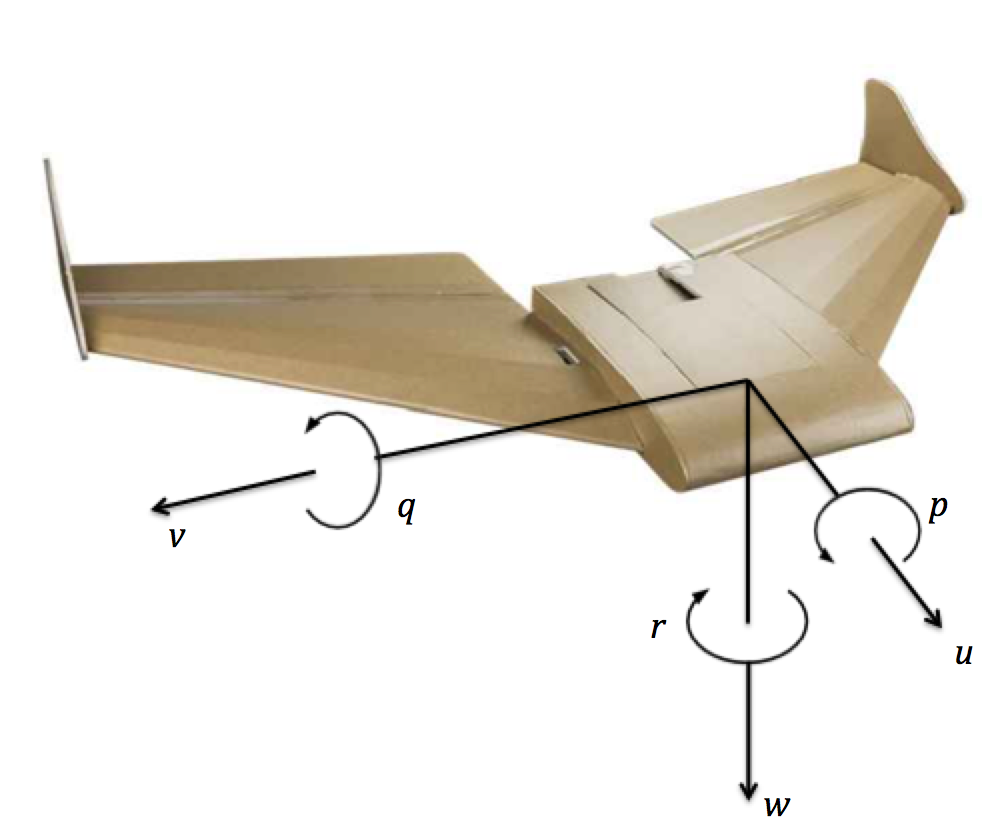
\includegraphics[width=0.65\textwidth]{body_frame_rotations.png}
  \caption{Reference frame - body rates and velocities}
  \label{fig:reference_frame}
\end{figure}

The primary goal of this research is to implement an algorithm which controls fixed wing attitude.  Therefore, the focus of the following kinematic and dynamics equations will primarily focus on deriving only rotational motion from first principles.  

Newton's second law as it pertains to rotational motion can be stated as
\begin{equation}\label{eq:rotational_inertia}
\tau=J\frac{d\omega}{dt_i}
\end{equation}

where $\tau$ is the torques applied to the body, $J$ is the moment of inertia, and $ \frac{d\omega}{dt_i}$ is the angular acceleration of the body with respect to the inertial frame.

Equation~\ref{eq:rotational_inertia} can be rewritten in the body reference frame as follows:

\begin{equation}
\tau^b=J\dot{\omega}_{b/i}^b+\omega_{b/i}^b\times\left(J\omega_{b/i}^b\right)
\end{equation}

The expression $\dot{\omega}_{b/i}^b$ is the angular acceleration in the body frame as viewed in the body frame:

\begin{equation}
\dot{\omega}_{b/i}^b=
\begin{pmatrix}
\dot{p}\\
\dot{q}\\
\dot{r}
\end{pmatrix}
\end{equation}

The equation can then be rewritten with respect to $\dot{\omega}_{b/i}^b$:

\begin{equation}
\dot{\omega}_{b/i}^b=J^{-1}\left[-\omega_{b/i}^b\times\left(J\omega_{b/i}^b\right)+\tau^b\right]
\end{equation}

$J$ can be defined as the inertia matrix as follows

\begin{equation}
J=
	\begin{pmatrix}
	J_x & -J_{xy} & -J_{xz}\\
	-J_{xy} & J_y & -J_{yz}\\
	-J_{xz} & -J_{yz} & J_z
	\end{pmatrix}
\end{equation}

The moments of inertia, or the diagonal terms, must be non-zero.  The products of inertia, or the off-diagonal terms, are terms which describe the coupling between axis.  For a traditional fixed wing aircraft, the natural symmetry will simplify the inertia matrix in the off-diagonal terms as follows:

\begin{equation}
J=
	\begin{pmatrix}
	J_x & 0 & -J_{xz}\\
	0 & J_y & 0\\
	-J_{xz} & 0 & J_z
	\end{pmatrix}
\end{equation}

The inverse of $J$ can be found to be

\begin{equation}
J^{-1}=
	\begin{pmatrix}
	\frac{J_z}{\Gamma} & 0 & \frac{J_{xz}}{\Gamma}\\
	0 & \frac{1}{J_y} & 0\\
	\frac{J_{xz}}{\Gamma} & 0 & \frac{J_x}{\Gamma}
	\end{pmatrix}
\end{equation}

where,

\begin{equation}
\Gamma = J_xJ_z-J_{xz}^2
\end{equation}

Aircraft nomenclature for torques are defined $\tau\triangleq(l,m,n)^T$ and therefore the combined equations derived from first principles take the form:

\begin{equation}\label{eq:body_rate_derivation}
\begin{split}
	\begin{pmatrix}
		\dot{p} \\
		\dot{q} \\
		\dot{r} 
	\end{pmatrix}
	&=
	\begin{pmatrix}
	\frac{J_z}{\Gamma} & 0 & \frac{J_{xz}}{\Gamma}\\
	0 & \frac{1}{J_y} & 0\\
	\frac{J_{xz}}{\Gamma} & 0 & \frac{J_x}{\Gamma}
	\end{pmatrix}
	\left[
	\begin{pmatrix}
		0& r& -q \\
		-r& 0& p \\
		q& -p& 0
	\end{pmatrix}
	\begin{pmatrix}
	J_x & 0 & -J_{xz}\\
	0 & J_y & 0\\
	-J_{xz} & 0 & J_z
	\end{pmatrix}
	\begin{pmatrix}
		p\\
		q\\
		r
	\end{pmatrix} +
	\begin{pmatrix}
		l\\
		m\\
		n
	\end{pmatrix}
	\right] \\	
	&=
	\begin{pmatrix}
		\frac{J_z}{\Gamma} & 0 & \frac{J_{xz}}{\Gamma}\\
		0 & \frac{1}{J_y} & 0\\
		\frac{J_{xz}}{\Gamma} & 0 & \frac{J_x}{\Gamma}
	\end{pmatrix}
	\left[
	\begin{pmatrix}
	J_{xz}pq+(J_y-J_z)qr\\
	J_{xz}(r^2-p^2)+(J_z-J_x)pr\\
	(J_x-J_y)pq-J_{xz}qr
	\end{pmatrix}+
	\begin{pmatrix}
		l\\
		m\\
		n
	\end{pmatrix}
	\right]\\	
	&=
	\begin{pmatrix}
		\Gamma_1pq-\Gamma_2qr+\Gamma_3l+\Gamma_4n\\
		\Gamma_5pr-\Gamma_6(p^2-r^2)+\frac{1}{J_y}m\\
		\Gamma_7pq-\Gamma_1qr+\Gamma_4l+\Gamma_8n
	\end{pmatrix}
	\end{split}		
\end{equation}
where,

\begin{equation}
\begin{split}
\Gamma_1&=\frac{J_{xz}(J_x-J_y+J_z)}{\Gamma}\\
\Gamma_2&=\frac{J_z(J_z-J_y)+J_{xz}^2}{\Gamma}\\
\Gamma_3&=\frac{J_z}{\Gamma}\\
\Gamma_4&=\frac{J_{xz}}{\Gamma}\\
\Gamma_5&=\frac{J_z-J_x}{J_y}\\
\Gamma_6&=\frac{J_{xz}}{J_y}\\
\Gamma_7&=\frac{J_x(J_x-J_y)+J_{xz}^2}{\Gamma}\\
\Gamma_8&=\frac{J_x}{\Gamma}\\
\end{split}
\end{equation}

The aerodynamic torques (excluding propulsive torques) can be found to be:

\begin{equation}\label{eq:aero_torques}
\begin{pmatrix}
		l\\
		m\\
		n
	\end{pmatrix}
	=
	\frac{1}{2}\rho V_a^2S
	\begin{pmatrix}
		b\left[C_{l_0}+C_{l_\beta}\beta+C_{l_p}\frac{b}{2Va}p+C_{l_r}\frac{b}{2V_a}r+C_{l_{\delta_a}}\delta_a+C_{l_{\delta_r}}\delta_r\right]\\
		c\left[C_{m_0}+C_{m_\alpha}\alpha+C_{m_q}\frac{c}{2V_a}q+C_{m_{\delta_e}}\delta_e\right]\\
		b\left[C_{n_0}+C_{n_\beta}\beta+C_{n_p}\frac{b}{2Va}p+C_{n_r}\frac{b}{2V_a}r+C_{n_{\delta_a}}\delta_a+C_{n_{\delta_r}}\delta_r\right]
	\end{pmatrix}
\end{equation}

Substituting the aerodynamic torques found in equation~\ref{eq:aero_torques} into equation~\ref{eq:body_rate_derivation} results in \cite{beard2012small}:
\begin{equation}\label{eq:body_rate_equations}
\begin{split}
	\dot{p}&=\Gamma_1pq-\Gamma_2qr+\frac{1}{2}\rho V_a^2Sb\left[C_{p_0}+C_{p_\beta}\beta+C_{p_p}\frac{bp}{2V_a}+C_{p_r}\frac{br}{2V_a}+C_{p_{\delta_a}}\delta_a+C_{p_{\delta_r}}\delta_r\right]\\
	\dot{q}&=\Gamma_5pr-\Gamma_6(p^2-r^2)+\frac{1}{2}\rho V_a^2Sc\frac{1}{J_y}\left[C_{m_0}+C_{m_\alpha}\alpha+C_{m_q}\frac{cq}{2V_a}+C_{m_{\delta_e}}\delta_e\right]\\
	\dot{r}&=\Gamma_7pq-\Gamma_1qr+\frac{1}{2}\rho V_a^2Sb\left[C_{r_0}+C_{r_\beta}\beta+C_{r_p}\frac{bp}{2V_a}+C_{r_r}\frac{br}{2V_a}+C_{r_{\delta_a}}\delta_a+C_{r_{\delta_r}}\delta_r\right]
\end{split}	
\end{equation}

Simplifying equation~\ref{eq:body_rate_equations} assuming no inertial or aerodynamic coupling results in:

\begin{equation}\label{eq:body_rate_simplified}
\begin{split}
	\dot{p}&=\frac{1}{2}\rho V_a^2Sb\left[C_{p_{\delta_a}}\delta_a+C_{p_p}\frac{bp}{2V_a}+C_{p_0}\right]\\
	\dot{q}&=\frac{1}{2}\rho V_a^2Sc\frac{1}{J_y}\left[C_{m_{\delta_e}}\delta_e+C_{m_q}\frac{cq}{2V_a}+C_{m_0}\right]\\
	\dot{r}&=\frac{1}{2}\rho V_a^2Sb\left[C_{r_{\delta_r}}\delta_r+C_{r_r}\frac{br}{2V_a}+C_{r_0}\right]
\end{split}	
\end{equation}

The equations in equation~\ref{eq:body_rate_simplified} are then slightly modified to fit the first order \ac{ODE} model as described in the primary literature \cite{hovakimyan2010l1}.
\begin{equation}\label{eq:simplified_ac_model}
\begin{split}
\hat{\dot{p}}&=A_p\hat{p}+b_p\left(\hat{\omega}_p\delta_a+\hat{\theta}_pp+\hat{\sigma}_p\right)\\
\hat{\dot{q}}&=A_q\hat{q}+b_q\left(\hat{\omega}_q\delta_e+\hat{\theta}_qq+\hat{\sigma}_q\right)\\
\hat{\dot{r}}&=A_r\hat{r}+b_r\left(\hat{\omega}_r\delta_r+\hat{\theta}_rr+\hat{\sigma}_r\right)
\end{split}
\end{equation}
where the hat nomenclature $(\text{ }\hat{}\text{ })$ recognizes that the parameters are estimates as follows,
\begin{itemize}
	\item[] $\hat{\omega}$ - estimated input gain coefficient
	\item[] $\hat{\theta}$ - estimated constant state coefficient
	\item[] $\hat{\sigma}$ - estimated disturbance estimate
\end{itemize}


\section{Classical Feedback vs Adaptive Control}
Control of a system can be broken into two required elements.  There is the requirement to control the system from:
\begin{enumerate}
	\item disturbances which affect the controlled states 
	\item disturbances which affect the performance of the system as a whole
\end{enumerate}
Classical feedback control seeks to solve the first type of disturbance.  This form of control is meticulously tuned to achieve the desired overshoot and settling time for example.  The important assumption that is made by classical feedback controllers is that the underlying plant/system performance is not changing.  For example the cruise control that maintains a vehicles speed assumes that the available horse power of the car is fixed.  This is a fairly good assumption as the horsepower with respect to rpm available at sea level and at 5,000 feet for an internal combustion engine is constant enough that a fixed gain feedback controller would perform well at maintaining the speed of the vehicle in both environments.  In the case of an airplane, the dynamic pressure is proportional to velocity squared and can drastically change the performance of the aircraft.  In this case, the constant system performance assumption can cause a fixed gain classical feedback controller to go unstable at higher dynamic pressures (higher airspeeds).   Conversely, adaptive controllers assume that the system performance is unknown and is likely to vary with time.  Adaptive control seeks to ensure a systems performance in terms of characteristics like damping ratio and settling time are kept constant regardless of a plant dynamics that may be unknown and time varying.  For both classical and adaptive control there exists some form of error which drives the controller.  In the case of classical feedback, the error is calculated between the command and the feedback state of the plant. In adaptive control (in general), the error is calculated between the outputs of the desired reference model and real plant's measured performance.

Figure~\ref{fig:why_adaptive_control} outlines the decision making process a controls engineer makes when deciding the type of controller needed for a given circumstance.

%I would not spend too much time here. What  critical is to demonstrate the fundamental difference. In the case of classical feedback the error is calculated between the command and the feedback of the plant. In adaptive control (in general) the error is calculated between the outputs of the reference model and real plant.


\begin{figure}[h!]
 \centering
  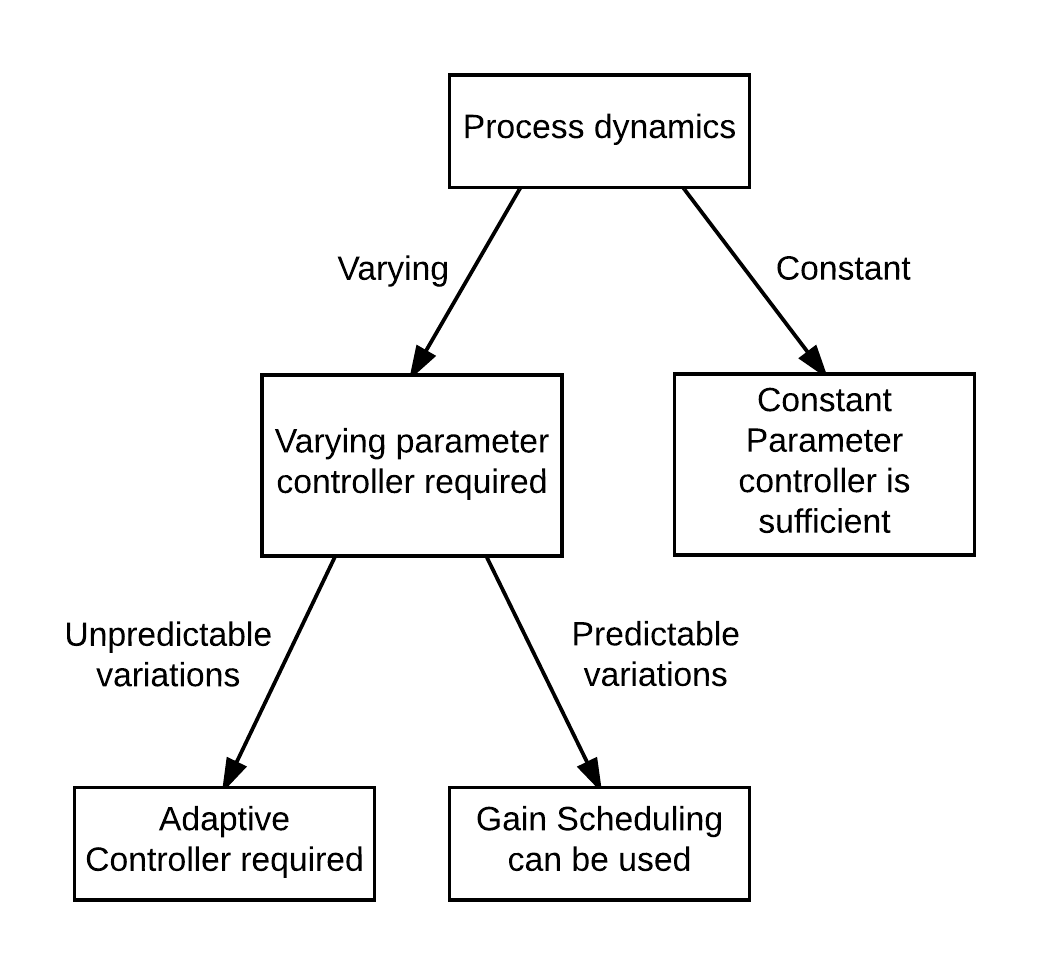
\includegraphics[width=0.5\textwidth]{why_adaptive_control.png}
  \caption{Determine if adaptive control should be used}
  \label{fig:why_adaptive_control}
\end{figure}


%---------------------------------------------------------
\section{Model Reference Adaptive Control}
\ac{MRAC} establishes the foundation for most of modern robust adaptive control.  Its structure is intuitive in nature and seeks to define a system's response to a command signal with a reference model.  Unlike traditional feedback where the error signal is generated with respect to state error, \ac{MRAC} attempts to achieve a system response with respect to some reference model performance. \ac{MRAC} assumes there there is some nominal response of the system which can be characterized with a model of unknown parameters.  The error between the model response and the system response generates the error for an 'adjustment mechanism' to learn the unknown model parameters.

\begin{figure}[h!]
 \centering
  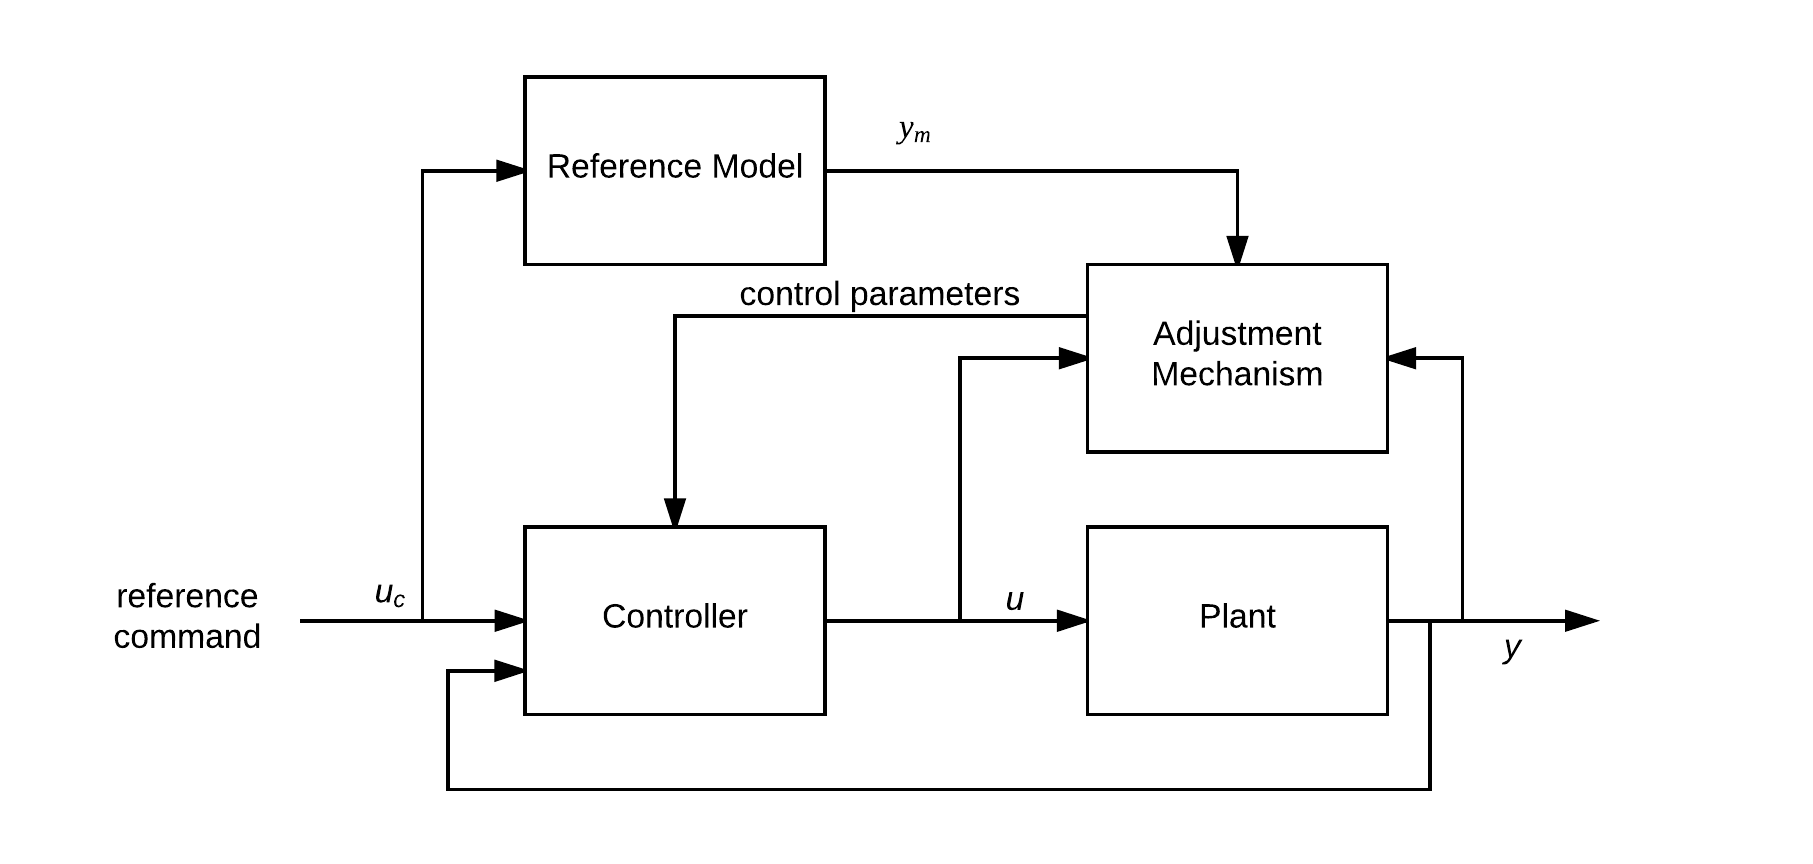
\includegraphics[width=1.0\textwidth]{traditional_MRAC.png}
  \caption{Traditional \ac{MRAC} architecture }
  \label{fig:traditional_mrac}
\end{figure}

Figure~\ref{fig:traditional_mrac} illustrates a topology where a traditional feedback controller is established as an inner loop and the 'Reference Model' and 'Adjustment Mechanism' is established as an outer loop.  The outer loop attempts to minimize the error between the reference model output and the plant output.  Using this error to learn the system parameters can be done utilizing one of two methods; gradient decent or stability theory.

\subsection{MIT Rule - Gradient Decent}
One of the first approaches to \ac{MRAC} controllers was implemented at the Instrument Labs at MIT (now known as Draper Labs).  The gradient decent based method was called the 'MIT Rule' for this reason \cite{aastrom2013adaptive}.  This method attempts to learn some unknown parameter by descending the gradient of the error between the reference model and the plant output.

Given the simple first order system $G(s)$:
\begin{equation}
G(s) = k_{dc}\frac{1}{s+1}
\end{equation}

where $k_{dc}$ is some unknown feedforward gain.  In the case of the MIT rule, $k_{dc}$ is the parameter to be learned and is defined as $\theta$.  The first step in the MIT rule is to establish a cost (or loss) function.  One example of a cost function $J(\theta)$ is:
\begin{equation}
J(\theta) = \frac{1}{2}e^2
\end{equation}
\begin{equation}
e=y-y_m
\end{equation}

where $e$ is error, $y$ is the plant output, and $y_m$ is the model output.

In order for the cost function to be minimized, the negative gradient of the cost function is calculated and used to correct the a priori estimate.  This method takes the following form where $\gamma$ is the adaptation gain:
\begin{equation}
\frac{d\theta}{dt}=-\gamma \frac{\partial{J}}{\partial{\theta}} =-\gamma e\frac{\partial{e}}{\partial{\theta}}
\end{equation}

The stability of this method is very system dependent and heavily relies on trial and error to ensure the adaptation gain $(\gamma)$ is not too high.  This usually requires low adaptation rates for most systems and may not produce adequate results.  It should also be noted that this method presupposes there is adequate persistence of excitation.  Without a frequency rich error signal being generated by adequate persistence of excitation, the model will fail to adapt.  This method also offers no guarantees that the learned parameters are actually the correct values.

\subsection{Lyapunov Stability Criteria}

Aerospace controllers tend to use linear controllers for their simplicity and well understood robustness characteristics.  This is despite the fact that the applications of these linear controllers are applied to a non-linear dynamical system such as attitude control with varying dynamic pressure.  Adaptive Controllers are non-linear and may offer performance benefits to non-linear systems as seen in aforementioned aerospace applications.  However, non-linear controller's robustness properties need to be evaluated.  The Lyapunov stability criteria offers methods of evaluating these controller's boundedness and robustness behavior.

Aleksandr Lyapunov was a Russian mathematician who's work was published in 1892 \cite{lyapunov1892general} concerning the behavior of non-linear systems close to equilibrium without having to rigorously find the unique solutions to difficult differential equations used to model the system.  His work was largely overlooked until the Cold War when aerospace solutions required a more rigorous approach to analyzing non-linear control robustness.  Modern non-linear control engineers extensively utilize Lyapunov's techniques to design and evaluate non-linear controllers.

\subsubsection{Lyapunov Stability Definitions}

Lyapunov's methods attempt to evaluate autonomous nonlinear dynamical systems within the bounds of three classifications.  In this case the autonomous system is defined as definable set of ordinary differential equations which are not explicitly dependent upon the independent variable.  These classifications can be used to define a nonlinear system as Lyapunov stable, asymptotically stable, or exponentially stable.

Given the following autonomous nonlinear dynamical system:

 \begin{equation}
\dot{x}(t)=f(x(t)), \qquad x(0)=x_0
\end{equation}

where $f$ has equilibrium at $x_e$ :
 \begin{equation}
f(x_e) = 0
\end{equation}

then the equilibrium is said to be:
\begin{enumerate}
	\item \textbf{Lyapunov Stable} \newline
	for every $\epsilon > 0$ there exists a $\delta > 0$ such that, if \: $\norm{x(0) - x_e} < \delta$, then for every $t \geq 0$ we have 	$ \norm{x(t) - x_e} < \epsilon$	
	\item \textbf{Asymptotically Stable} \newline
	if the system is Lyapunov stable and there exists a $\delta > 0$ such that if \: $\norm{x(0) - x_e}  < \delta$, then $\displaystyle \lim_{t\to \infty} \norm{x(t)-x_e} =0$
	\item \textbf{Exponentially Stable} \newline
	if the system is asymptotically stable and there exists $\alpha > 0, \beta > 0, \delta > 0$ such that if $\norm{x(0)-x_e}<\delta$, then \:$\norm{x(t)-x_e} \leq \alpha \norm{x(0)-x_e} e^{-\beta t}$, for all $t \geq 0$
\end{enumerate}

Being Lyapunov stable infers that if a system is near equilibrium then it will indefinitely remain near equilibrium.  If the system if found to be asymptotically stable then it eventually will achieve equilibrium as $t\to \infty$ and being exponentially stable implies it reaches equilibrium even faster.

\subsubsection{Lyapunov's Second Method}
 
Lyapunov's second proposed method is also known as Lyapunov stability criteria.  This method offers a less tenuous method for evaluating mathematically non-ideal systems.  Lyapunov analysis of the linearized system around equilibrium can be cumbersome in the case where equilibrium is at the origin or the eigenvalues are purely imaginary.  In this case, the solutions can rapidly depart to infinity or approach zero with little perturbation to the eigenvalues.  Lyapunov's second method offers an alternative approach for classifying a systems stability using a concept that is similar to how energy is defined in classical dynamics.

Conceptually, Lyapunov's second method can be compared to evaluating the energy of a vibrating spring mass system.  The energy of the unforced spring mass system will dissipate energy due to friction and or damping etc.  This trend of energy leaving the system towards some 'attractor' is evidence of the system's stability characteristics and identifies that there will be some stable end state.  Like wise, Lyapunov's second method characterizes this with the use of a Lyapunov candidate function $V(x)$.  It is important to note that Lyapunov realized that the candidate function can be any function so as long as one candidate function is found in agreement with the stability criteria.  It is then said to be Lyapunov stable if any candidate equation is found and meets the stability criteria.  This means that it is only incumbent upon the engineer to find one candidate equation to meet the criteria.  This can be an iterative process of trying multiple energy like equations.  A common approach is to model the Lyapunov candidate equation as kinetic energy $(\frac{1}{2}u^2)$.  Lyapunov realized that characterizing the energy of a nonlinear system could be almost impossible for some cases, but this approach could prove stability without the rigorous knowledge of the true system's energy.

Lyapunov's second method defines a system as Lyapunov Stable for a system $\dot{x}=f(x)$ having an equilibrium point at $x=0$ where the Lyapunov candidate function $V(x):\mathbb{R}^n \rightarrow \mathbb{R}$ such that:
\begin{itemize}
	\item $V(x)=0$ if and only if $x=0$
	\item $V(x)>0$ if and only if $x\neq0$
	\item $\dot{V}(x)=\frac{d}{dt}V(x)=\sum\limits_{i=1}^{n} \frac{\partial V}{\partial x_i}f_i(x) \leq 0$, for all values of $x\neq 0$		
\end{itemize}

if $\dot{V}(x) < 0$ for $x\neq 0$ then system is asymptotically stable.

To determine if the system is globally stable, it is additionally required to prove the condition of radial unboundedness.















 	%Background and Literature Review
\chapter{\Lone Adaptive Control Derivation}\label{ch:derivation}

Introduction here!!!

\section{\Lone Adaptive Control}
The \Lone adaptive controller is an evolution of the concepts implemented by \ac{MRAC}.  They are similar approaches designed to model a \ac{LTI} system with unknown constant parameters.  These parameters are adjusted to achieve the desired outcome of the error between the actual plant (system) and the referenced system model (state predictor) to asymptotically approach zero.   Adaptive control attempts to estimate the plant's unknown parameters in situ.  Parameter estimation is done using either direct or indirect architecture.  The indirect architecture attempts to estimate the system's parameters, which could be considered similar to system identification.  Alternately the easier to implement direct architecture estimates the controller parameters explicitly.  These architectures can be seen below in Figures~\ref{fig:direct_mrac} and \ref{fig:indirect_mrac}.

\begin{figure}[h!]
 \centering
  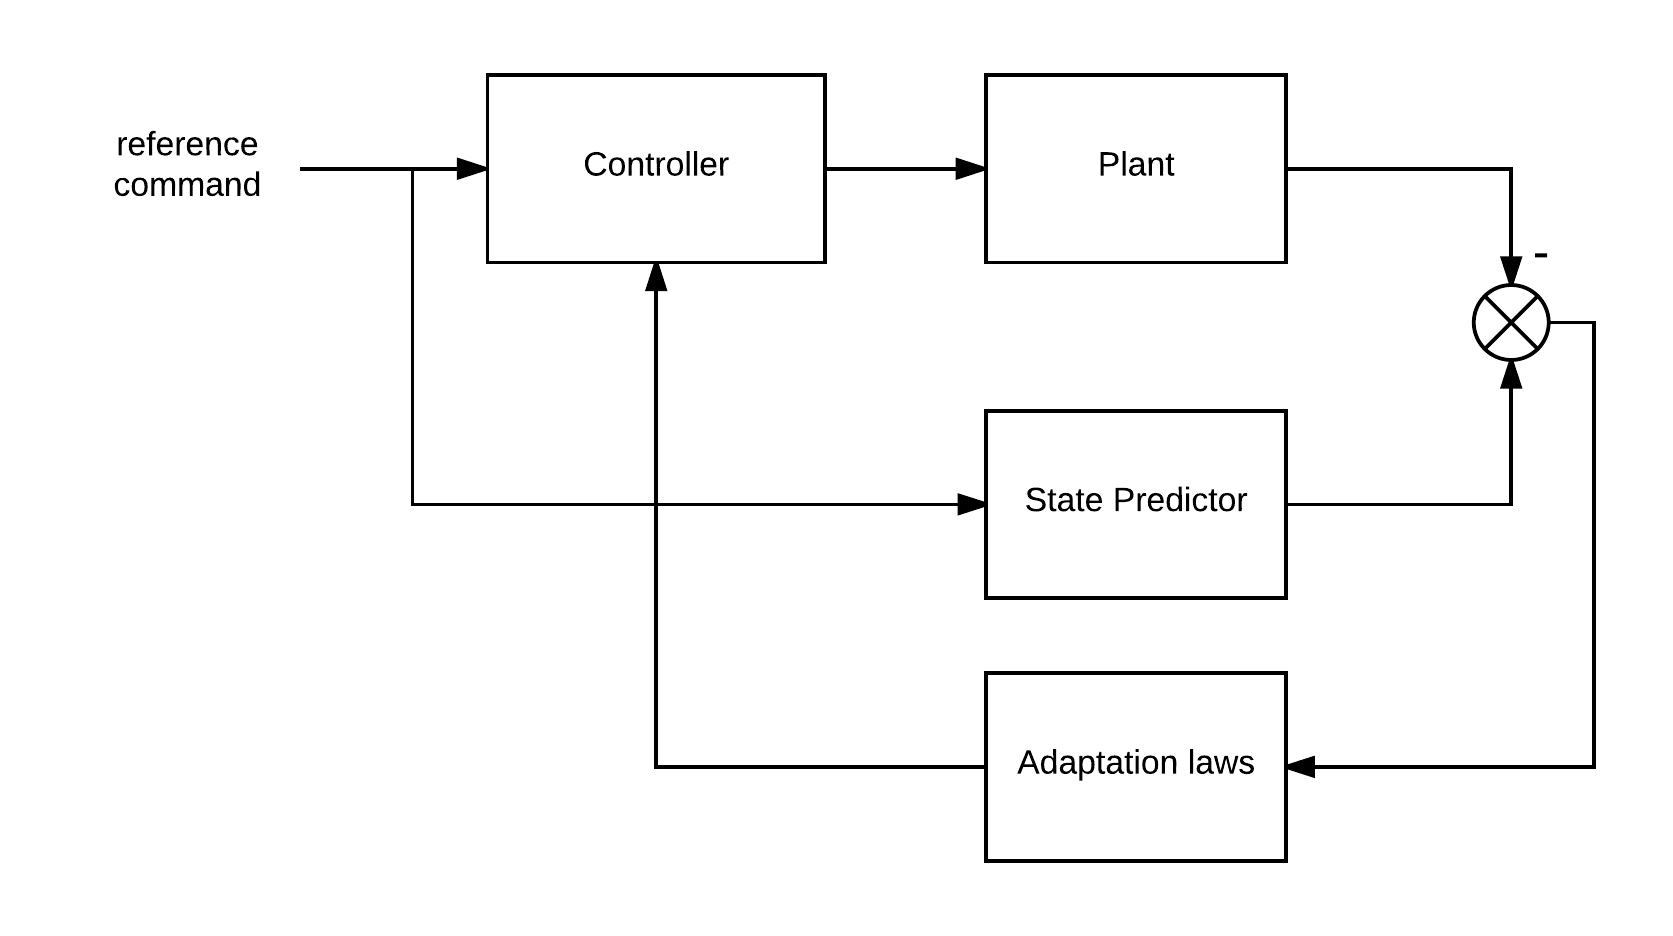
\includegraphics[width=0.75\textwidth]{Direct_MRAC.png}
  \caption{Direct \ac{MRAC} architecture }
  \label{fig:direct_mrac}
\end{figure}

\begin{figure}[h!]
 \centering
  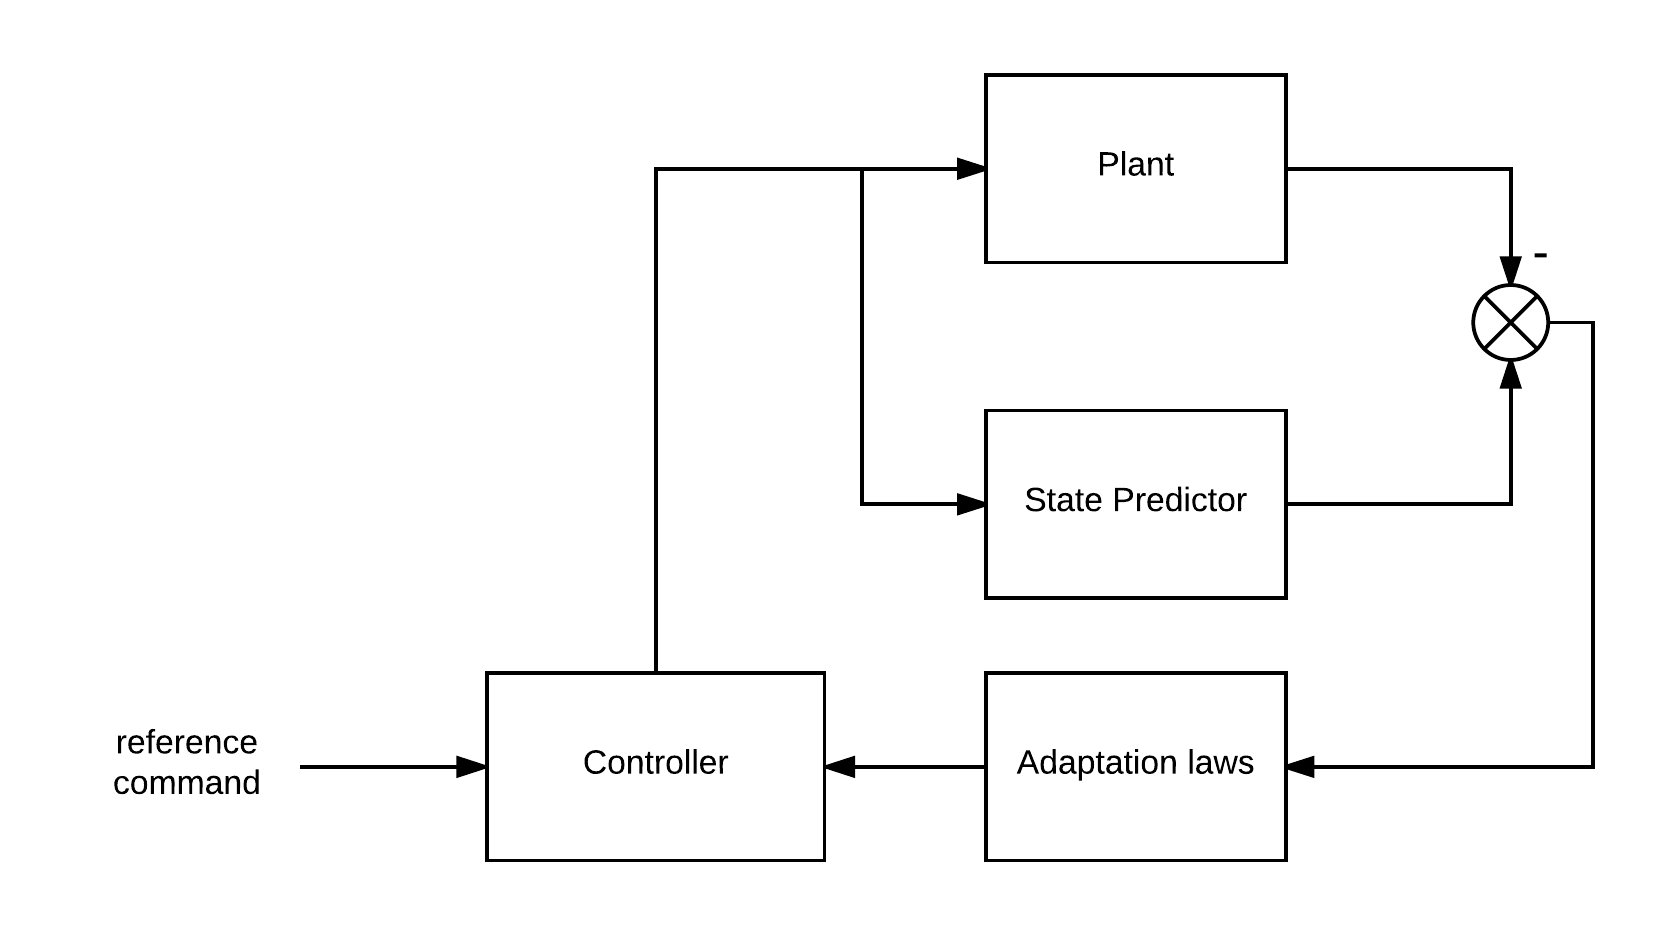
\includegraphics[width=0.75\textwidth]{Indirect_MRAC.png}
  \caption{Indirect \ac{MRAC} architecture }
  \label{fig:indirect_mrac}
\end{figure}

\subsection{Reference Model versus Companion Model}
Traditional \ac{MRAC} controllers often refer to the system objective function as the 'Reference Model.'  In this case, the engineer designs a reference model response, and it is from this model response that the error state is calculated directly.  Because the \Lone adaptive control implements the use of a low-pass filter in conjunction with a model objective function, the model is often referred to as the 'Companion Model.'  This subtle distinction is necessary because the engineer must be aware that the system response will be the with respect to the low-pass filter and the companion model in series.  In other words, the plant will not mimic the companion model; it will mimic the companion model plus the low-pass filter.

\subsection{\Lone Architecture}
The \Lone adaptive control algorithm asserts that trying to estimate the plant uncertainties outside of the control actuators' bandwidth is overly ambitious.  The system's actuator bandwidth and the slow dynamics of the plant are most commonly the system's limiting factors, and the estimator's robustness/stability could be in question if unmodeled high-frequency content exists in the plant.  % See RHORs example here? 
The \Lone adaptive control constrains the objective function by using a low-pass filter (first or second order) to band the frequency response in order to meet robustness specifications.  This low-pass filter should be tuned to a frequency response commensurate with the actuator's frequency response.  Through inspection the low-pass filter placement in the controller topology, it becomes clear that the indirect architecture is the only candidate as detailed below.  Figures~\ref{fig:direct_mrac_lowpass} and \ref{fig:indirect_mrac_lowpass} illustrate the placement of the low-pass filter and its implication on the closed loop model. 

\begin{figure}[h!]
 \centering
  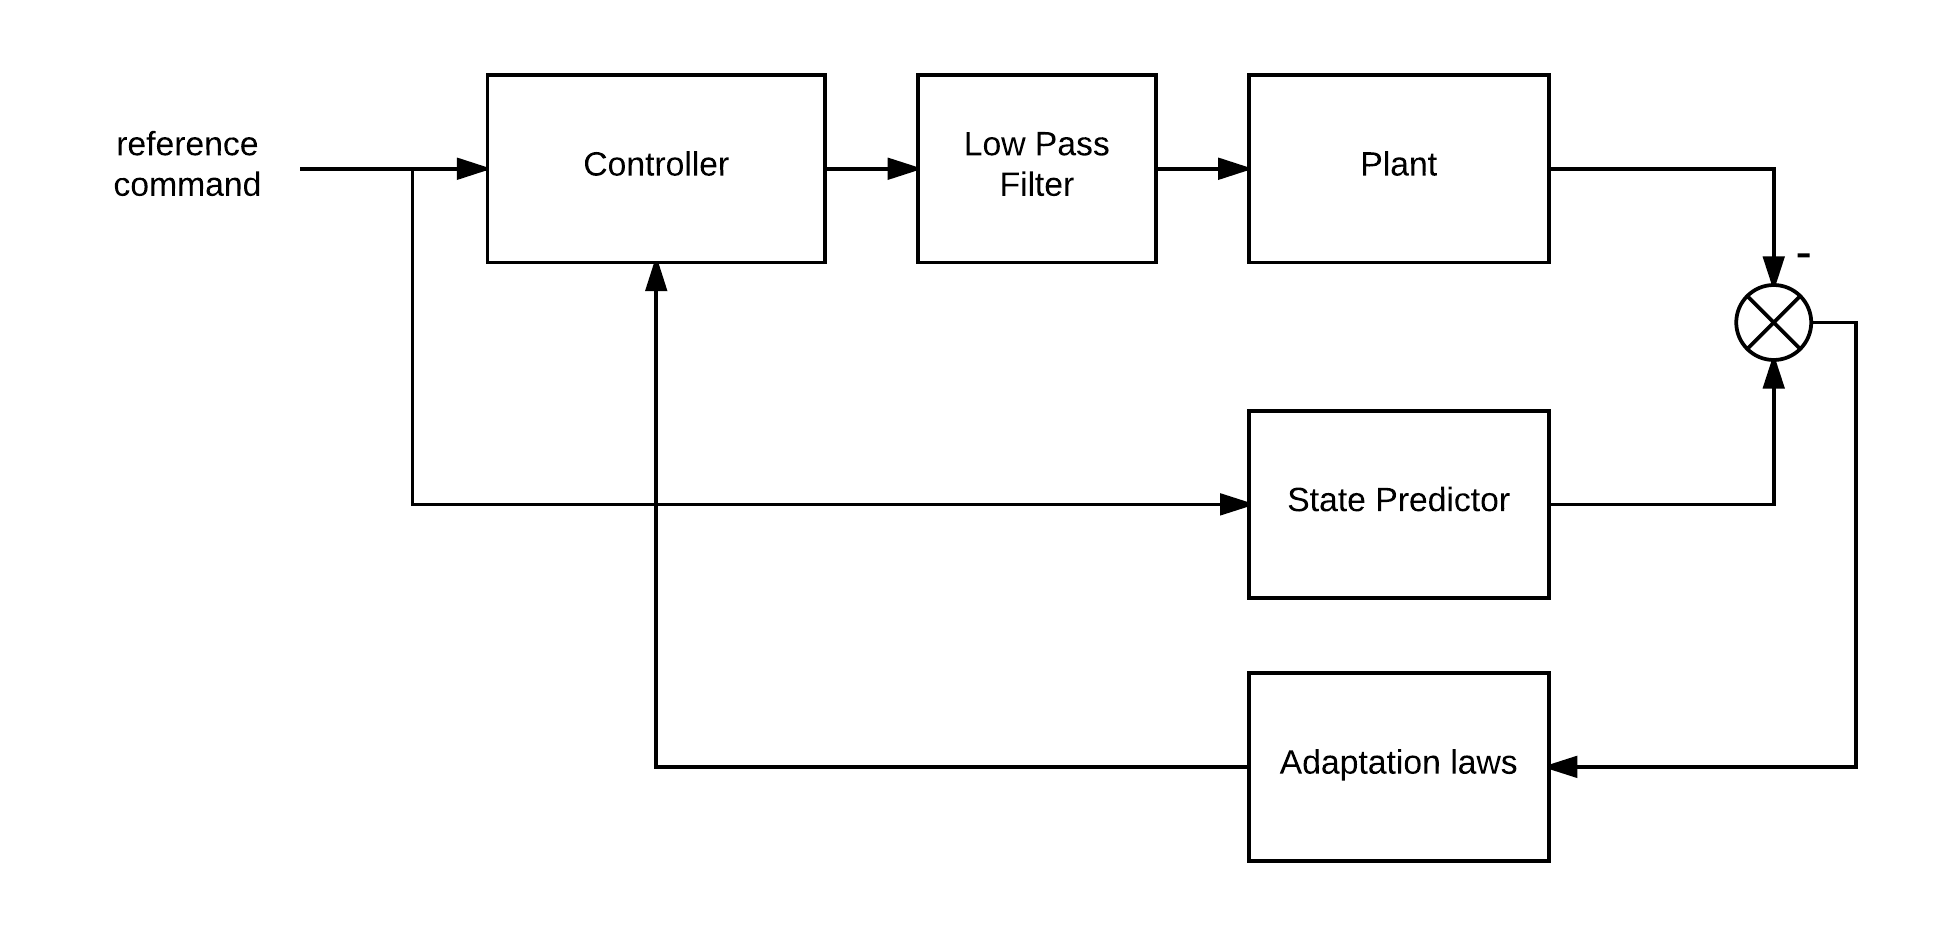
\includegraphics[width=0.75\textwidth]{Direct_MRAC_lowpass.png}
  \caption{Direct \ac{MRAC} architecture with low-pass filter }
  \label{fig:direct_mrac_lowpass}
\end{figure}
 It can be seen in figure~\ref{fig:direct_mrac_lowpass} that the direct architecture implementation of the low-pass filter introduces difficulties.  The low-pass filter cascades with the plant and effectively creates a new plant that is simply the plant plus a low-pass filter.  The aerodynamic and Lyapunov stability underpinnings become non-sensical in this implementation and are non-subtractable when the error state is calculated.
\begin{figure}[h!]
 \centering
  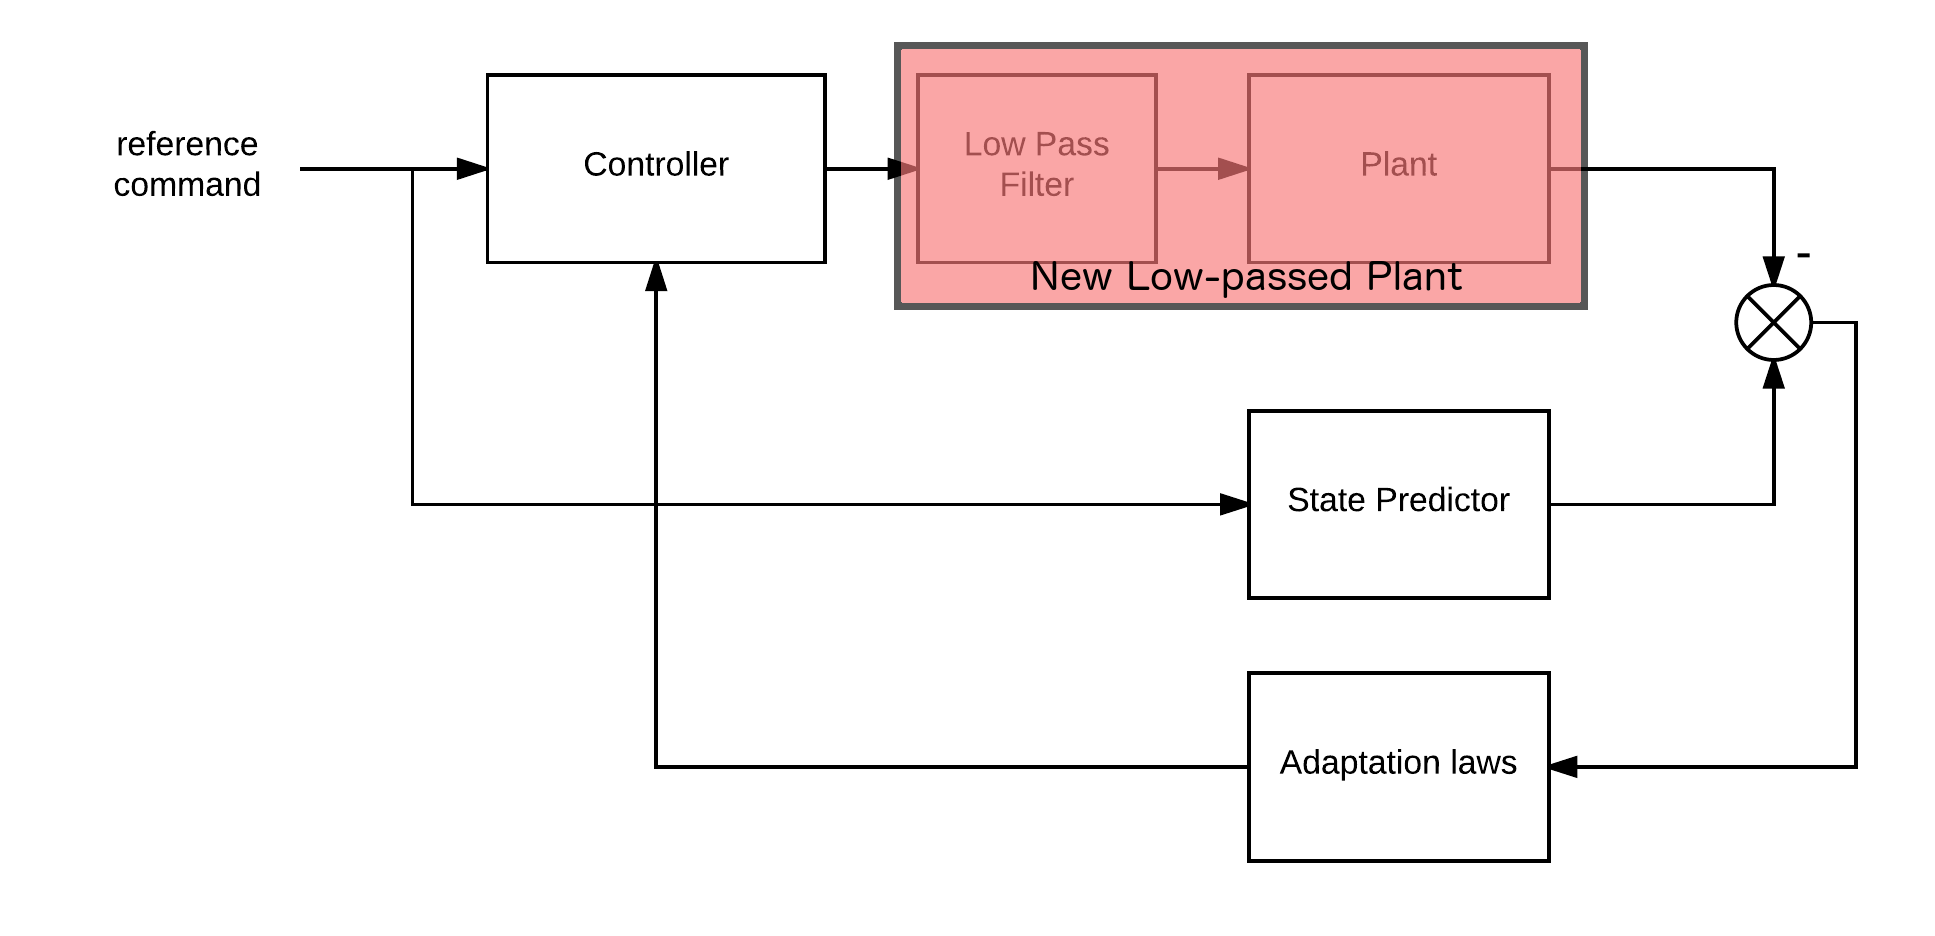
\includegraphics[width=0.75\textwidth]{Direct_MRAC_lowpass_plant.png}
  \caption{Non-Subtractable Lowpass Implementation - Direct Architecture}
  \label{fig:direct_mrac_lowpass}
\end{figure}

Conversly, the indirect approach offers an implementation which ensures the low-pass filter is applied to both the companion model (state predictor) and the plant.
\begin{figure}[h!]
 \centering
  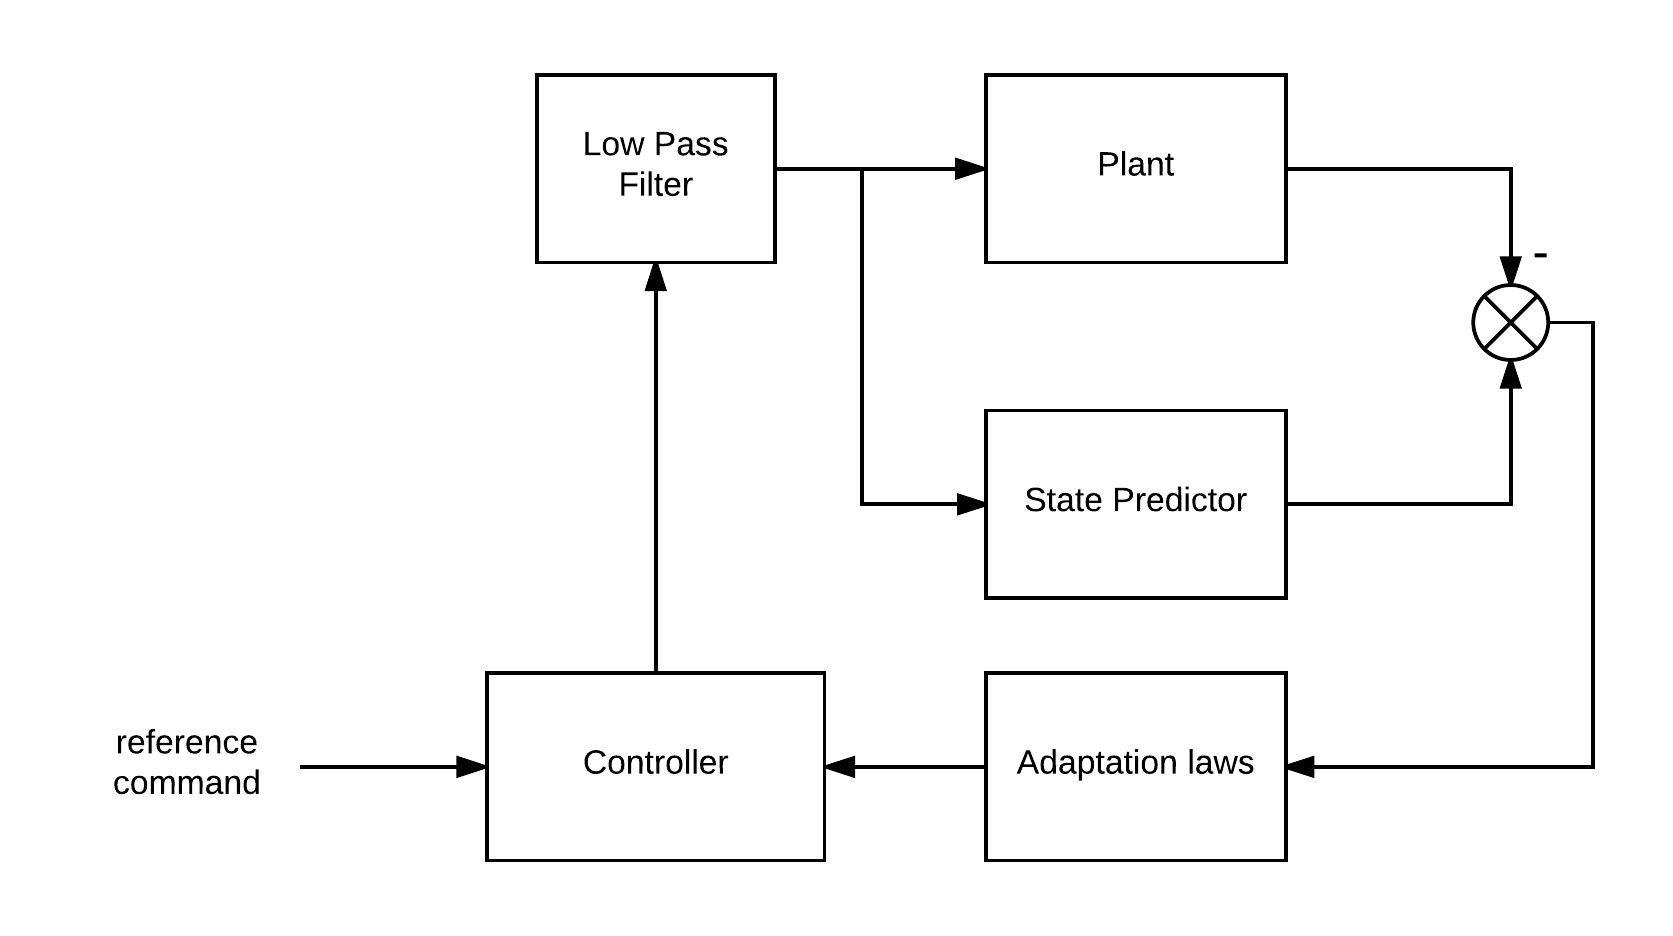
\includegraphics[width=0.75\textwidth]{Indirect_MRAC_lowpass.png}
  \caption{Indirect \ac{MRAC} architecture with low-pass filter }
  \label{fig:indirect_mrac_lowpass}
\end{figure}

 It can be seen that the low-pass filter in the direct architecture inherently changes the structure of the model with the cascading of the low-pass filter and plant block diagrams.  This change mathematically is not mirrored in the companion model (state predictor) and therefore is not subtractable.  However, in the indirect case, the structure of the model is kept intact and the low-pass filter is applied to both the plant and the state predictor.  This ensures that the low-pass filter is subtractable when calculating the error state and the model's structure is kept intact.

Many slight variations of the \Lone adaptive architectures have been derived for various use cases \cite{hovakimyan2010l1}.  Some of the following forms were studied for viability in the fixed wing \ac{UAS} use case:
\begin{itemize}
 \item \ac{SISO} with constant but unknown state parameters
 \item \ac{SISO} with time variant and/or nonlinear unknown state parameters
 \item \ac{MIMO} with constant but unknown state parameters
 \item \ac{MIMO} with time variant and/or nonlinear unknown state parameters
\end{itemize}

\ac{MIMO} control algorithms would potentially afford the controller more ability to cope with system coupling if present.  A fixed wing \ac{UAS} would exhibit coupled behavior due to the coupling present in the aerodynamics as seen in equation~\ref{eq:aero_torques}, but was not chosen due to the added architectural complexity.  Unknown state parameters that are assumed to be constant or time invariant are considered matched uncertainty.  Unknown state parameters that are non-constant (time variant) and/or exhibit non-linear behavior are considered unmatched uncertainty.  The unmatched uncertainty architecture offers a more appealing solution for fixed wing use cases (asymmetric actuator failure, aerodynamic coefficients scaled by dynamic pressure, etc.), but adds a significant amount of complexity to the architecture.  In summary, the \ac{SISO} architecture with matched uncertainty was chosen for this research.  

The \ac{SISO} controller with matched uncertainty was chosen to control pitch rate $(q)$ and roll rate $(p)$ of the aircraft using two separate, but parallel controllers.  This meant that the controller could be generalized to a first principles physical point mass model similar to derivations found in rigid body equations of motion.  In this implementation of the \Lone adaptive controller, the desired state $x$ to be controlled was an individual body rate (\eg $q$, $p$). 

\begin{figure}[h!]
 \centering
  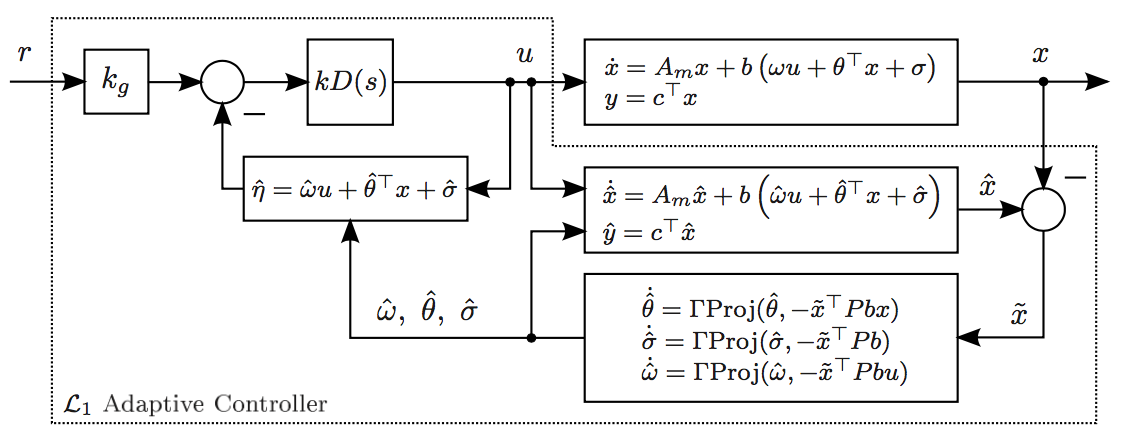
\includegraphics[width=1.0\textwidth]{L1_architecture.png}
  \caption{\Lone Architecture with Matched Uncertainty Block Diagram \cite{hovakimyan2010l1} }
  \label{fig:l1_architecture}
\end{figure}

As seen in Figure~\ref{fig:l1_architecture}, the generalized \Lone architecture in block diagram form and the following elements can be identified:
\begin{itemize}
 \item[] $k_g$ - feed forward input gain
 \item[] $k$ - feedback gain
 \item[] $D(s)$ - user described filter (second order low pass plus integrator)
 \item[] $\hat{\eta}$ - \Lone controller state
 \item[] $\dot{x}$ - first order differential equation of state model
 \item[] $\hat{x}$ - state estimate
 \item[] $\tilde{x}$ - state error
 \item[] $u$ - controller output
 \item[] $r$ - reference objective
 \item[] $A_m$ - Hurwitz matrix
 \item[] $b$ - input matrix
 \item[] $\hat{\omega}$ - unknown input gain coefficient
 \item[] $\hat{\theta}$ - unknown constant state coefficient
 \item[] $\hat{\sigma}$ - unknown disturbance estimate
 \item[] $\Gamma$ - adaptation gain
 \item[] $Pb$ - solution to the Lyapunov stability criterion 
\end{itemize}

It should also be noted that the architecture presented in Figure~\ref{fig:l1_architecture} includes the use of a projection operator.  The parameters for $\dot{\hat{\omega}}$, $\dot{\hat{\theta}}$, and $\dot{\hat{\sigma}}$ are all projection based adaptation laws.  This ensures that the adaptation stays bounded around the feasible region of parameter space.  The Lyapunov stability proofs for this architecture rely on this method to guarantee stability\cite{hovakimyan2010l1}.  More discussion on the specific application of this operator can be found in Appendix~\ref{appendix:projection_derivation}.

One of the main benefits of using the \ac{SISO} architecture is that the solution to the Lyapunov stability criterion ($Pb$) used in the projection based adaptation laws is greatly simplified.  

In this case, $Pb$ reduces to:
\begin{equation}
Pb = \frac{1}{2\omega_n}
\end{equation}

where $\omega_n$ is the natural frequency in rad/s for the first order companion model in discrete recursive form assuming DC gain of 1.  The proof for this can be found in Appendix~\ref{sec:projection_proof}.

%---------------------------------------------------
\section{\Lone Parameter Estimation}\label{sec:param_estimation}
Three Parameters are estimated in this research with increasing complexity both in architecture and in required stability proofs.  The following outlines the nomenclature for the estimation of a system with unknown constant parameters, input/output disturbances, and an unknown system input gain.

The \Lone adaptive control algorithm is primarily used to estimate unknown constant system parameters.  These system parameters are defined as $\theta$ as seen in the following model:
\begin{equation}
\dot{x}(t)=Ax(t)+b(u(t)+\theta^{\top}(t)x(t))
\end{equation}

The second adaptive element is the estimation of the input/output disturbances $(\sigma)$.  This additional parameter is implemented in this research as any unmodeled transient dynamics such as aerodynamic/inertial coupling.  This model takes the form:
\begin{equation}
\dot{x}(t)=Ax(t)+b(u(t)+\theta^{\top}(t)x(t)+\sigma(t))
\end{equation}

The last adaptive element used for this research was the estimation of unknown system input gain $(\omega)$.  Estimating the unknown system input gain offers the controller the ability to estimate the actuator effectiveness for changes in dynamic pressure or failed control surfaces.  This model takes the form:
\begin{equation}\label{eq:l_one_model}
\dot{x}(t)=Ax(t)+b(\omega(t)u(t)+\theta^{\top}(t)x(t)+\sigma(t))
\end{equation}  

The above model in equation~\ref{eq:l_one_model} can be paralleled to the aircraft model derived in equation~\ref{eq:simplified_ac_model} as follows for the roll rate model example below:

\begin{equation}
 \hat{\dot{p}}=A_p\hat{p}+b_p\left(\hat{\omega}_p\delta_a+\hat{\theta}_pp+\hat{\sigma}_p\right)
\end{equation}

This final model, with the inclusion of all three estimated parameters $(\hat{\omega}, \hat{\theta}, \hat{\sigma})$, established the architecture tested in this research.  The fundamental assumption that the aerodynamic and inertial coupling was negligible and set to zero as outlined in equation~\ref{eq:body_rate_simplified} is agreeably a gross assumption which may prove to be inadequate for stable flight.  These assumptions presume that the estimated input/output disturbance $(\hat{\sigma})$ would be adequate to compensate for these unmodeled dynamics and were validated by successful flight test in section~\ref{sec:flight_test}.

%---------------------------------------------------
\section{\Lone Filter - $C(s)$}
One of the key features of the \Lone adaptive controller is that the robustness of the controller is decoupled from the adaptation rate.  This is handled in the filter section of the \Lone architecture.  One of the elements that the guaranteed stability depends upon is that $C(s)$ is strictly-proper stable.  With the architecture that includes the system input gain $(\omega)$, one cannot simply apply a stand alone filter.  The inclusion of $\omega$ in the architecture block diagram in figure~\ref{fig:l1_architecture} slightly modifies the signal output and takes the following form:
\begin{equation}
u(s)=-kD(s)(\hat{\eta}(s)-k_gr(s))
\end{equation}
where $D(s)$ is the new user defined filter and $C(s)$ now takes the form:
\begin{equation}
\begin{split}
\omega \in \Omega_0 \triangleq [\omega_{l_0},\omega_{u_0}]\\
C(s)=\frac{\omega kD(s)}{1+\omega kD(s)}
\end{split}
\end{equation}

In the case where the user defined function $D(s)$ is a simple integrator, $C(s)$ takes the form:
\begin{equation}\label{eq:l1_filter}
\begin{split}
D(s)&=\frac{1}{s}\\
C(s)&=\frac{\omega k}{s+\omega k}
\end{split}
\end{equation}

The feedback gain $k$ should not be assumed to be 1 in this case.  As seen in equation~\ref{eq:l1_filter}, the $C(s)$ transfer function is a function of $k$ that can have significant influence on the controller output.  In actual implementation, $k$ was found to be one of the most influential gains in the architecture and extremely critical in specifying the transition between robustness and performance.


%---------------------------------------------------
\section{\Lone Discrete Time Implementation}
Implementing any algorithm on actual autopilot hardware will inevitably force some if not all parts of the algorithm to be discretized.  Autopilots like the Pixhawk operate at some scheduled loop rate for executing the litany of subprograms that measure sensors, calculate navigation commands, and much more.  In the case of the Pixhawk autopilot, you can run the main loop up to 400 Hz.  At 400 Hz, there is a significant insurance that the vehicle's full frequency domain of importance will be achievable.  However, the \ac{APM} flight stack records all logged parameters also at this loop rate and can create log files larger than are reasonably desired.  There are a myriad of other reasons why the engineer would not want to run at high loop rates, but successful flight at the lowest (default of 50Hz) is desired if adequate performance of the adaptive control can be achieved.  Failures in early adaptive control were largely in part due to a very naive understanding of robustness.  Brian Anderson concludes that "it is clear that the identification time scale needs to be faster than the plant variation time scale, else identification cannot keep up" \cite{anderson2005failures}.  

The \Lone architecture does not require the algorithm to run in sync with the sensor measurements etc.  Ideally, the autopilot main loop rate would remain at its default value (50Hz), and the adaptation section of the \Lone controller would run as fast as the CPU would allow.  However, the \ac{APM} architecture doesn't lend itself well to this scheme in its current configuration without significant modification to the code base.  Therefore, the initial tests will presume that the \Lone algorithm is running at the same frequency as the main loop of the autopilot.  The fundamental derivation of the \Lone algorithm proves that performance and adaptation gain are maximized as the loop time (dt) approaches zero.  Increased performance would come from higher adaptation loop rates, but the primary focus was to implement the \Lone algorithm with minimal or no detrimental effects to the current \ac{APM} codebase.

\subsection{Digital Bi-Quad Filter}

The \Lone adaptive control algorithm utilizes two specific elements that will require careful discretization; the companion model and the low pass filter.  The digital bi-quad filter offers a very versatile and straightforward method for accurately implementing the companion model and the low pass filter discretely using its recursive nature.  It is a second order filter which uses a \ac{FIR} front end and an \ac{IIR} back end requiring 4 total memory blocks.  This topology allows the designer to create numerous types of filters (low pass, high pass, bandpass, etc) simply by choosing appropriate coefficients.  If a first order filter is needed then the higher order FIR/IIR terms can be set to zero.  Figure~\ref{fig:bi-quad} illustrates this filter's topology where the \ac{FIR} structure is the left two memory blocks and the \ac{IIR} structure is the right two memory blocks.

\begin{figure}[h!]
 \centering
  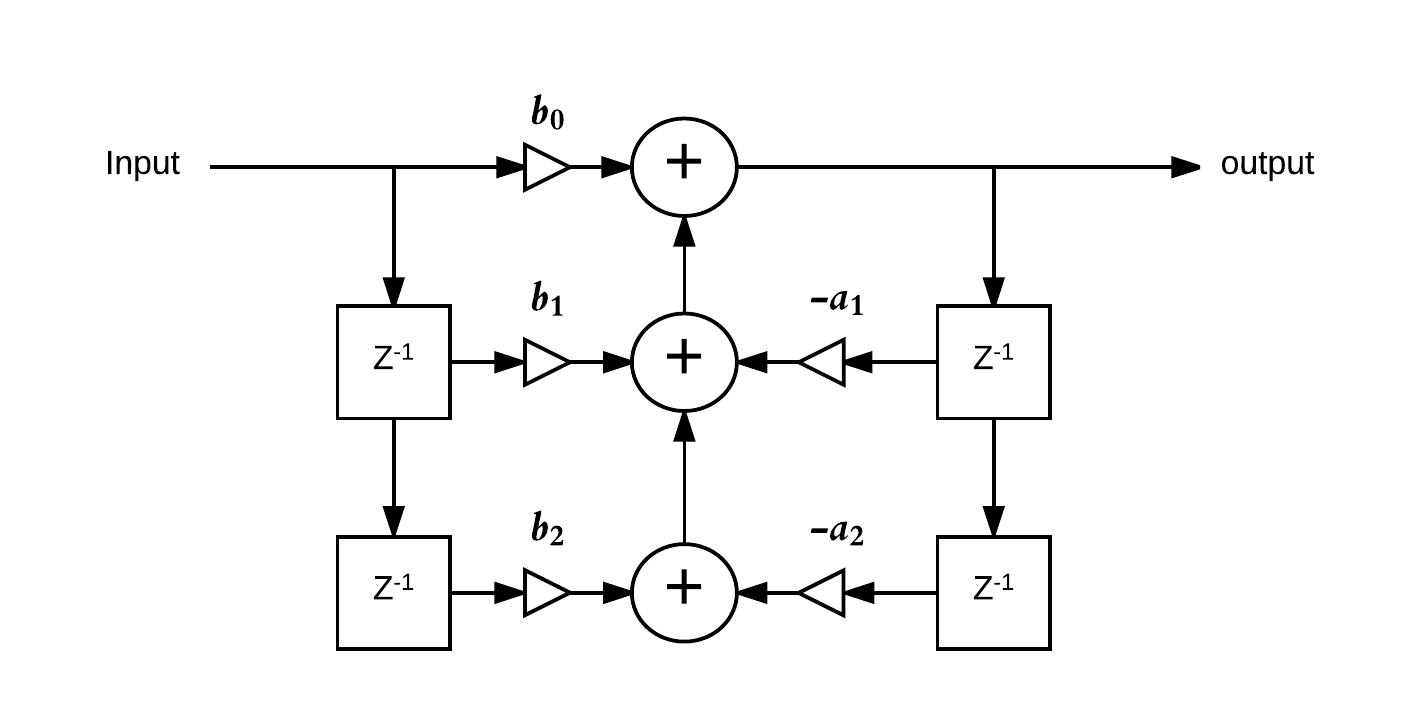
\includegraphics[width=1.0\textwidth]{bi-quad_filter.png}
  \caption{Digital Bi-quad Filter Architecture }
  \label{fig:bi-quad}
\end{figure}

To determine the structure of the coefficients, a bilinear Z transform is used to convert the desired S-domain (continuous time domain) filter/model into the Z-domain (discrete time domain).  

\begin{figure}[h!]
 \centering
  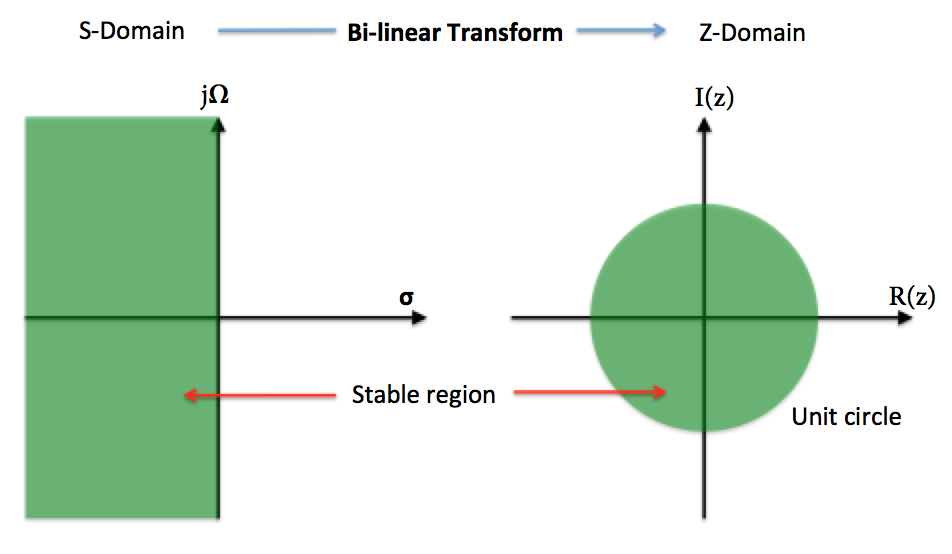
\includegraphics[width=1.0\textwidth]{bi-linear_transform.png}
  \caption{Bi-linear Transform}
  \label{fig:bi-linear_transform}
\end{figure}

This derivation can be seen below for the second order low pass model:

\begin{equation}
 H(s) = \frac{1}{s^2+\frac{s}{Q}+1}
\end{equation}

where the bi-linear transform converts s to z via:

\begin{equation}
 s = \left(\frac{1}{K}\right)\left(\frac{z-1}{z+1}\right)
\end{equation}

$K$ is the 'pre-warping' factor which accounts for the transition of the vertical s-plane into the circular z-plane as seen in figure~\ref{fig:bi-linear_transform}.

where $\omega T$ is:

\begin{equation}
 \omega T = 2\pi\left(\frac{F_c}{F_s}\right)
\end{equation}

\begin{equation}
\begin{split}
 K &= tan\left(\frac{\omega T}{2}\right) \\
 &= tan\left(\pi\frac{F_c}{F_s}\right)
\end{split}
\end{equation}



$F_c$ is the desired corner frequency of the filter and $F_s$ is the sampling rate (or loop rate of the autopilot).
This 'pre-warping' is critical to ensure that the continuous time cutoff frequency desired is correctly established in the discrete implementation.  It is the engineer's discretion if pre-warping is required for the appropriate application, but the general guidance is to pre-warp the Z-domain coefficients if the desired cut-off frequency is close to Nyquist.  It was chosen for this application to always pre-warp the coefficients even though the error is small for corner frequencies which are fairly distant from Nyquist.  This was chosen simply because calculating the $tan()$ function real time on the CPU adds negligible computational strain but offers ease of tuning for the engineer.

Applying the bi-linear transform to the continuous time second order low pass filter results in:

\begin{equation}\label{eq:bi-linear}
 H(z) = \frac{1}{ \left[\left(\frac{1}{K}\right)\left(\frac{z-1}{z+1}\right)\right]^2+\frac{ \left(\frac{1}{K}\right)\left(\frac{z-1}{z+1}\right)}{Q}+1}
\end{equation}

The desired form is:

\begin{equation}\label{eq:bi-quad}
 H(z) = \frac{b_0 + b_1 z^{-1} + b_2 z^{-2}}{a_0 + a_1 z^{-1} + a_2 z^{-2}}
\end{equation}

Reducing equation~\ref{eq:bi-linear} to match the form in equation~\ref{eq:bi-quad} results in the following coefficients:

\begin{equation}
\begin{split}
 a_0 &= 1 \\
 a_1 &= \frac{2(K^2-1)}{K^2+\frac{K}{Q}+1} \\
 a_2 &= \frac{K^2-\frac{K}{Q}+1}{K^2+\frac{K}{Q}+1} \\
 b_0 &= \frac{K^2}{K^2+\frac{K}{Q}+1} \\
 b_1 &= 2b_0 \\
 b_2 &= b_0  
\end{split}
\end{equation}

The bandwidth of the filter $Q$ can be set by the engineer.  For example, if the pass-band of the filter is desired to be flat (Butterworth) then $Q$ can be set equal to $\frac{1}{\sqrt{2}}$.  For this research, the following C++ code segments were used to explicitly calculate the bi-quad low-pass filter implementation: \newline

\begin{lstlisting}
void DigitalBiquadFilter<T>::compute_params(float sample_freq, 
float cutoff_freq, biquad_params &ret) {
    ret.cutoff_freq = cutoff_freq;
    ret.sample_freq = sample_freq;

    float fr = sample_freq/cutoff_freq;
    float K = tanf(M_PI/fr);  //Pre-Warp calculation
    float c = 1.0f+2.0f*cosf(M_PI/4.0f)*K + K*K;

    ret.b0 = K*K/c;
    ret.b1 = 2.0f*ret.b0;
    ret.b2 = ret.b0;
    ret.a1 = 2.0f*(K*K-1.0f)/c;
    ret.a2 = (1.0f-2.0f*cosf(M_PI/4.0f)*K+K*K)/c;
}
\end{lstlisting}

\begin{lstlisting}
T DigitalBiquadFilter<T>::apply(const T &sample, 
const struct biquad_params &params) {
    
    T delay_element_0 = sample - _delay_element_1 * params.a1 
     - _delay_element_2 * params.a2;
    
    T output = delay_element_0 * params.b0 
     + _delay_element_1 * params.b1 
     + _delay_element_2 * params.b2;

    _delay_element_2 = _delay_element_1;
    _delay_element_1 = delay_element_0;

    return output;
}

\end{lstlisting}

This implementation can be used as the \Lone low-pass filter and as the companion model.  It can be seen in the above code segment that $K$, the pre-warp factor, is explicitly calculated every iteration.

\subsection{Simplified Bi-quad First Order Model}

In the case of the companion model, a first order response may be desired.  As described in equations~\ref{eq:first_order_model} and \ref{eq:state_space_model}, the discrete first order model can be derived from a simplified Bi-quad as seen below in figure~\ref{fig:bi-quad_first_order}.  It can be seen that the first coefficient of the \ac{IIR} filter is kept from this topology.
\begin{figure}[h!]
 \centering
  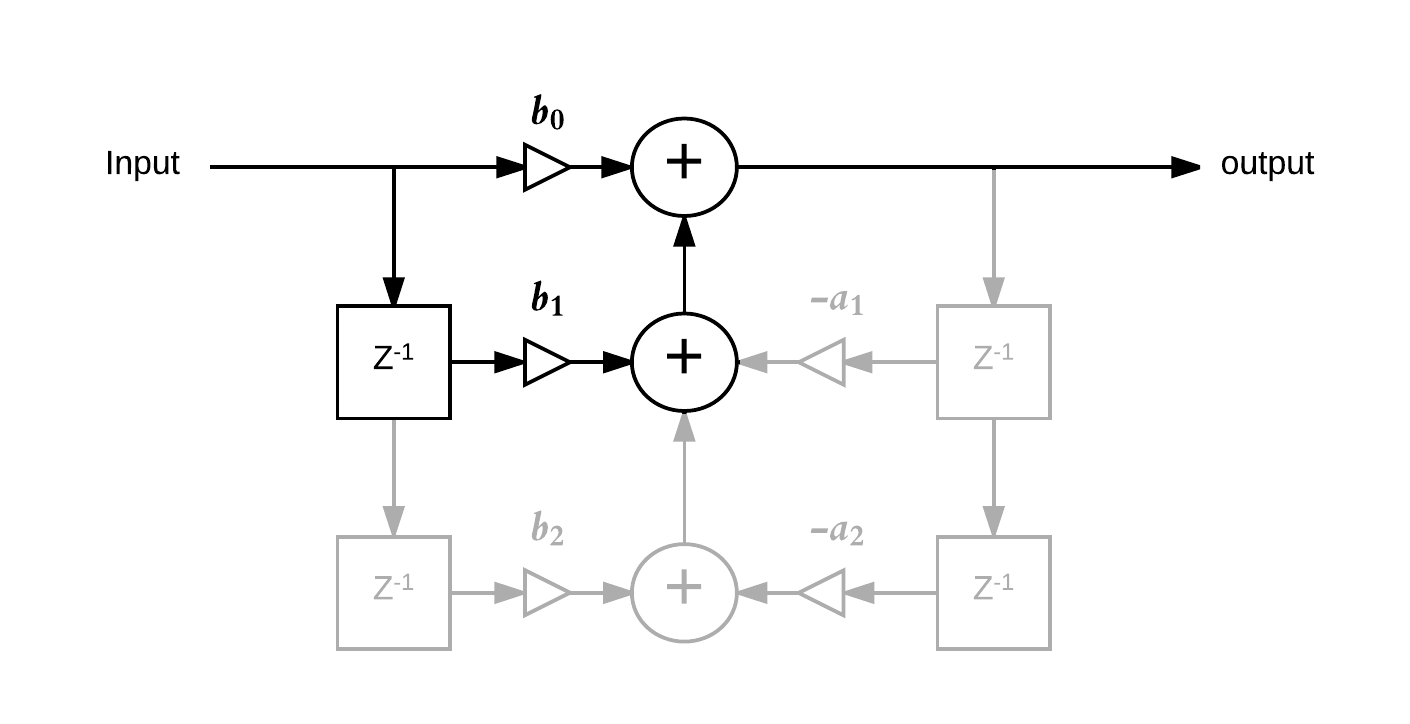
\includegraphics[width=1.0\textwidth]{bi-quad_first_order.png}
  \caption{Digital Bi-quad Simplified First Order Low-pass Filter }
  \label{fig:bi-quad_first_order}
\end{figure}

The first order model can be specified by either its time constant (time in seconds to reach 63\% of steady state) or its -3dB corner frequency.  The system takes the form as seen in equation~\ref{eq:first_order_corner_model} when defined by its corner frequency.

\begin{equation}\label{eq:first_order_corner_model}
H(s)=\frac{\omega_n}{s+\omega_n}
\end{equation}

therefore the explicit calculation of the Bi-quad coefficients in this case becomes:

\begin{equation}\label{eq:first_order_coeffieicnts}
\begin{split}
 a_1&=e^{\left(\frac{-\omega_n}{F_s}\right)}  \\
 b_0&=1-a_1
\end{split}
\end{equation}

where $\omega_n$ is the -3dB corner frequency in radians per second and $F_s$ is the sampling frequency in Hz.

Therefore the discrete recursive form of the first order model becomes:

\begin{equation}
y_{i+1}=a_1y_{i-1}+b_0y_i
\end{equation}

Another form designed to optimize for speed that is commonly seen in software takes the form:

\begin{lstlisting}
float b_0=exp(-f_c/f_s);
float out+=(in-out)*b_0;
\end{lstlisting}

\subsection{Euler vs Trapezoid Rule}

The model estimate, as well as the parameter estimates for the \Lone algorithm, are both numerically estimated using discrete integration.  The Euler method is a numerical procedure for solving ordinary differential equations. The Euler method as applied to discrete integration is the fundamental method for recursively integrating a digital signal.  The algorithm takes the form: \newline
where $h$ is the uniform step size,
\begin{equation}
y_{i+1}=y_i+hf(t_i,y_i)
\end{equation}

The recursive trapezoidal method takes the form:
\begin{equation}\label{eq:trapezoidal_integration}
\begin{split}
\tilde{y}_{i+1}&=y_i+hf(t_i,y_i) \\
y_{i+1}&=y_i+\frac{h}{2}[f(t_i,y_i)+f(t_{i+1},\tilde{y}_{i+1})]
\end{split}
\end{equation}

Comparing the accuracy of the two numerical methods for discretely calculating the integral of $y=e^t$ can be seen in figure~\ref{fig:trapezoidal_integration}:

\begin{figure}[h!]
 \centering
  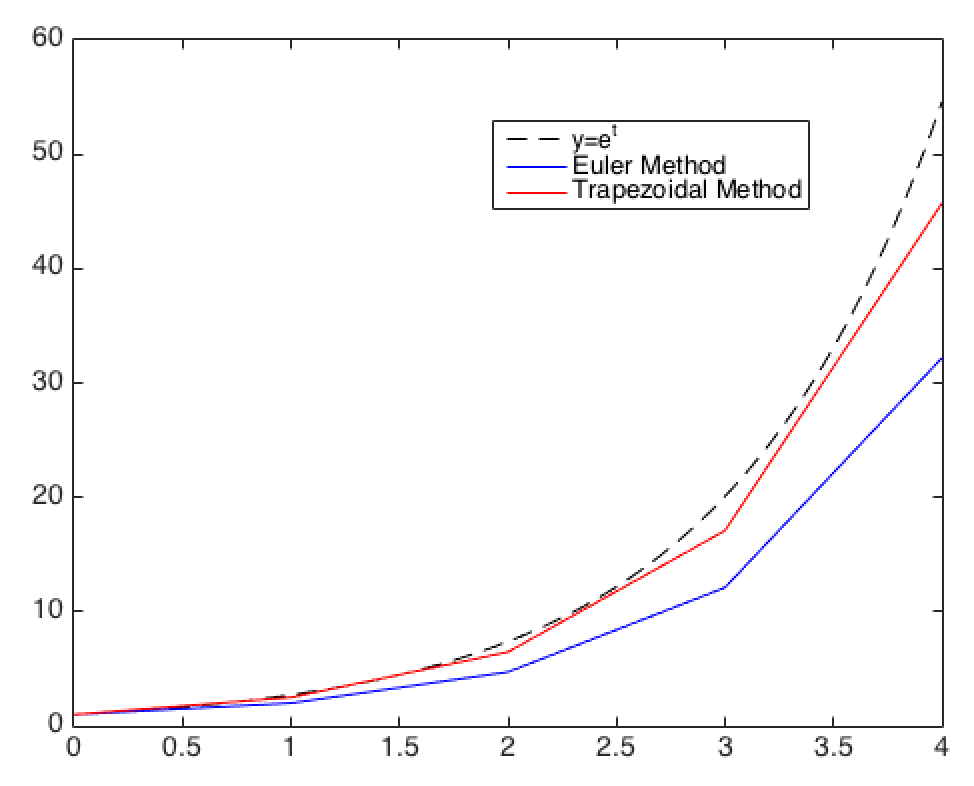
\includegraphics[width=0.75\textwidth]{trapezoidal_integration.png}
  \caption{Euler vs Trapezoidal Integration error}
  \label{fig:trapezoidal_integration}
\end{figure}

As seen in equation~\ref{eq:trapezoidal_integration}, the recursive trapezoidal integration method only adds one more line of complexity to the algorithm for a significant gain in accuracy and therefore will be the chosen method applied for all discrete numerical integration in this research and takes the form: \newline

\begin{lstlisting}
float trap_integration(float y0, float y1_dot, float dt, float &y0_dot)
{
    float y1 = y0 + (dt/2)*(y0_dot+y1_dot);
    y0_dot = y1_dot;

    return y1;
}
\end{lstlisting}












	%L1 Adaptive Control Derivation
\chapter{Design of Experimental Platform}\label{ch:platform}

This chapter presents the \ac{COTS} autopilots used in this research as well as outlining the Linux toolchain used to conduct |ac{SITL} and \ac{GCS} operations.  This chapter also introduces the airframes that were prototyped for testing specific performance characteristics discussed in Chapter~\ref{ch:performance}.

\section{Pixhawk Autopilot}
The Pixhawk autopilot is a collaborative project among open-source engineers which resulted in a high-performance autopilot which is capable of controlling aircraft, ground vehicles, and many others.  The primary reason this autopilot was chosen was because of the vast amount of support in the developer community.  The Pixhawk 1 autopilot hardware is effectively obsolete at the time of this writing, but the open-source code base is extremely flexible and continues to be ported to new hardware as it becomes available.  This has been the case for various Raspberry Pi autopilots as well as the Pixhawk 2.  The Pixhawk autopilot operates using two flight stacks (code base/operating systems); the PX4 flight stack and the \ac{APM} flight stack.  This research was implemented on the \ac{APM} flight stack primarily because the author's familiarity with the developer team which offers unparalleled assistance to the academic community.  The \ac{APM} codebase also offers a litany of open-source tools such as a Linux based \ac{GCS}, \ac{SITL} simulator, log analysis tools, and an \ac{API} for the RealFlight 7.5 simulator (high fidelity airframe simulation for small aircraft).

Figure~\ref{fig:pixhawk_autopilot} illustrates the connection diagram for the Pixhawk 1 autopilot.

\begin{figure}[h!]
 \centering
  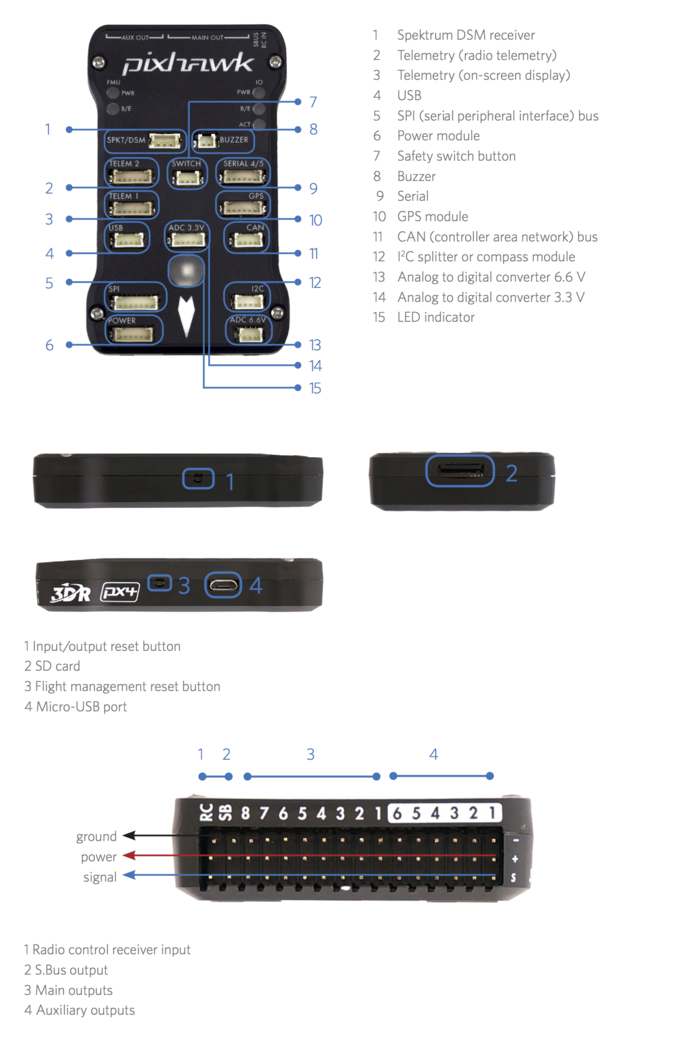
\includegraphics[width=0.65\textwidth]{pixhawk_connectors.png}
  \caption{Pixhawk 1 Autopilot Connection Diagram.  Source \cite{apm_org}.}
  \label{fig:pixhawk_autopilot}
\end{figure}

\subsection{Key Features}
The Pixhawk 1 Autopilot has the following features as found on \cite{apm_org}:
\begin{itemize}
\item 168 MHz / 252 MIPS Cortex-M4F
\item 14 PWM / Servo outputs (8 with failsafe and manual override, 6 auxiliary, high-power compatible)
\item Abundant connectivity options for additional peripherals (UART, I2C, CAN)
\item Integrated backup system for in-flight recovery and manual override with dedicated processor and stand-alone power supply (fixed-wing use)
\item Backup system integrates mixing, providing consistent autopilot and manual override mixing modes (fixed wing use)
\item Redundant power supply inputs and automatic failover
\item External safety switch
\item Multicolor LED main visual indicator
\item High-power, multi-tone piezo audio indicator
\item microSD card for high-rate logging over extended periods of time
\end{itemize}

\subsection{Specifications}
The Pixhawk 1 Autopilot has the following specifications as found on \cite{apm_org}:
\subsubsection{Processor}
\begin{itemize}
\item 32bit STM32F427 Cortex M4 core with FPU
\item 168 MHz
\item 256 KB RAM
\item 2 MB Flash
\item 32 bit STM32F103 failsafe co-processor
\end{itemize}
\subsubsection{Sensors}
\begin{itemize}
\item ST Micro L3GD20H 16 bit gyroscope
\item ST Micro LSM303D 14 bit accelerometer / magnetometer
\item Invensense MPU 6000 3-axis accelerometer/gyroscope
\item MEAS MS5611 barometer
\end{itemize}
\subsubsection{Interfaces}
\begin{itemize}
\item 5x UART (serial ports), one high-power capable, 2x with HW flow control
\item 2x CAN (one with internal 3.3V transceiver, one on expansion connector)
\item Spektrum DSM / DSM2 / DSM-X® Satellite compatible input
\item Futaba S.BUS® compatible input and output
\item PPM sum signal input
\item RSSI (PWM or voltage) input
\item I2C
\item SPI
\item 3.3 and 6.6V ADC inputs
\item Internal microUSB port and external microUSB port extension
\end{itemize}

\section{Ground Control Station}

The \ac{GCS} used for this research was MAVproxy \cite{mavproxy}.  It is an open-source python based \ac{GCS} which provides flexible communication and command with any autopilot utilizing the MAVlink protocol \cite{mavlink}.  Even though MAVproxy is written in Python (\ac{OS} agnostics language), it was found to be cumbersome to operate the \ac{GCS} on any other platform other than Linux.  This is primarily because the source code updates quite rapidly to support new features and the core developer (Andrew Tridgell) exclusively utilizes MAVproxy in Linux.  A significant amount of external libraries are utilized which results in a moderate amount of compatibility debugging for other \ac{OS}'s if desired.

\subsection{MAVproxy Features}
The following are summaries which proved to be extremely useful for this research \cite{mavproxy_wiki}:
\begin{itemize}
\item command-line, console based application. Plugins included in MAVProxy provide a basic \ac{GUI}.
\item network capable and run over any number of computers.
\item portable; capable of running on any POSIX OS with Python, pyserial, and select() function calls, which means Linux, OS X, Windows, and others.
\item light-weight design; runs on small netbooks.
\item tab-completion of commands.
\end{itemize}

\section{Simulation}
The \ac{APM} environment offers three versions of \ac{SITL} simulations.  The lowest fidelity \ac{SITL} is provided by MAVproxy, which is a simple 6-degree of freedom kinematics model with no environment or actuator modeling.  This proved to be adequate for initial testing but resulted in poorly tuned algorithms when actual flight tests were conducted.  The MAVproxy simulator was used for basic code debugging but nothing else.

The second \ac{SITL} offered in the \ac{APM} environment is X-plane 10.  This is a much higher fidelity simulation, which includes actuator models and environmental modeling.  X-plane 10 is primarily used for simulating full-scale aircraft and therefore is difficult to find models, which accurately represent the dynamics of small fixed-wing \ac{UAS}.  The open-source community provided model called the \enquote{maxi-swift} was similar enough to the airframe in this research that it provided adequate \ac{SITL} modeling which ensured robust flight test.

The last \ac{SITL} simulation tested under the \ac{APM} environment was the RealFlight 7.5 \ac{API}.  The RealFlight \ac{RC} airplane simulator offers some of the industry's highest fidelity simulations for small aircraft.  This product requires an \ac{API} key to hook into MAVproxy.  This capability is not yet on the market as of the time of this research, but the \ac{APM} core developers were supportive of this research and ran multiple experiments with the RealFlight \ac{SITL} for early validation.  The screenshot in Figure~\ref{fig:realflight_sitl} was captured while conducting testing utilizing the RealFlight \ac{SITL}.

\begin{figure}[h!]
 \centering
  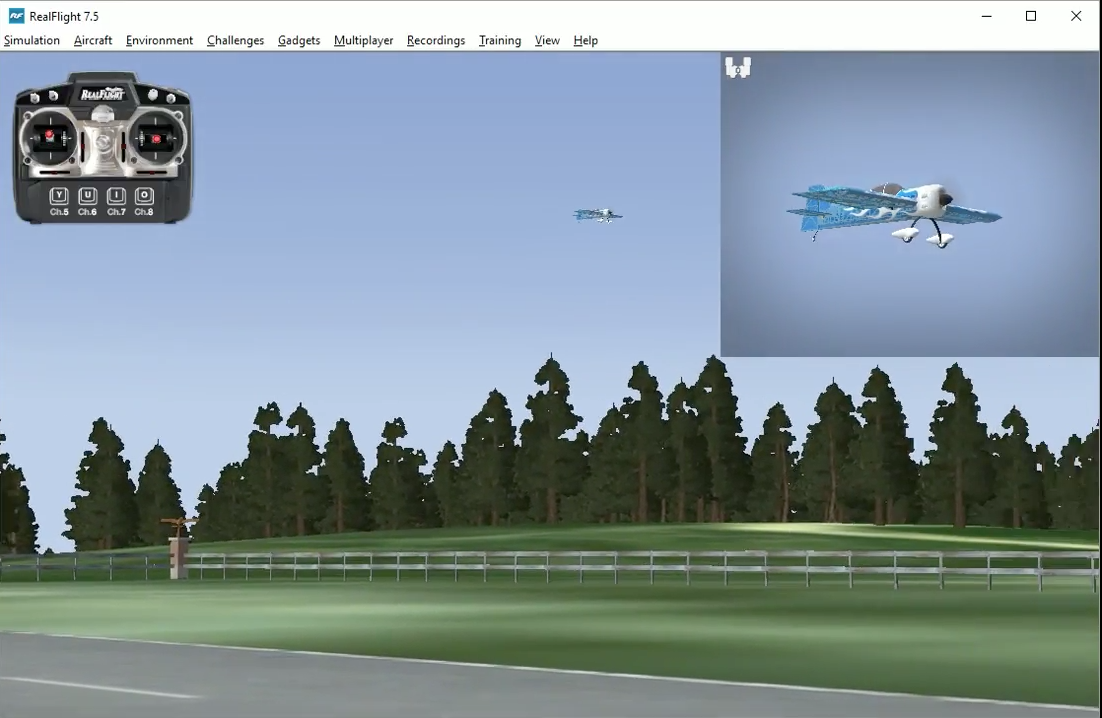
\includegraphics[width=0.65\textwidth]{realflight_simulator.png}
  \caption{High Fidelity RealFlight 7.5 Software in the Loop (SITL)}
  \label{fig:realflight_sitl}
\end{figure}


\section{Airframe}

The aircraft used for this research was the Flitetest Spear and the Flitetest Explorer \cite{flitetest}.  The Spear airframe was chosen for its endurance capability of greater than 45 minutes of flight time and its large capacity fuselage.  The flying-wing architecture keeps the actuation requirement to a minimum of two servos by utilizing an elevon configuration.

Figures~\ref{fig:spear} and \ref{fig:spear_cargo} are example photos from the instructional build website \cite{flitetest}.  Figure~\ref{fig:spear_build} illustrates the process of building the Spear aircraft.  The large blunt nose provides adequate space for two 2,200 mAh (12.6volts) lithium polymer batteries wired in parallel.  The remaining cargo space was used for accommodating the Pixhawk autopilot.

\begin{figure}[!h]
 \centering
  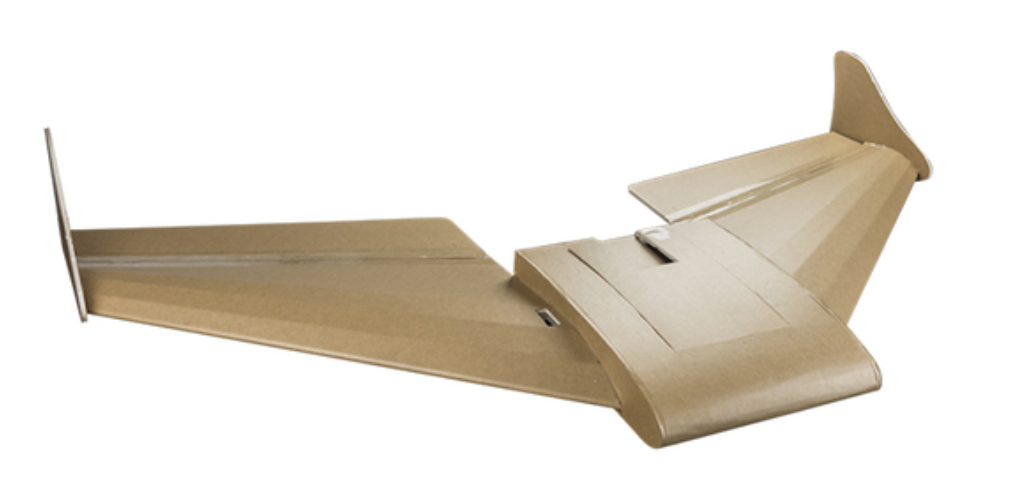
\includegraphics[width=0.65\textwidth]{spear.png}
  \caption{Spear Airframe.  Source \cite{flitetest}.}
  \label{fig:spear}
\end{figure}

\begin{figure}[!h]
 \centering
  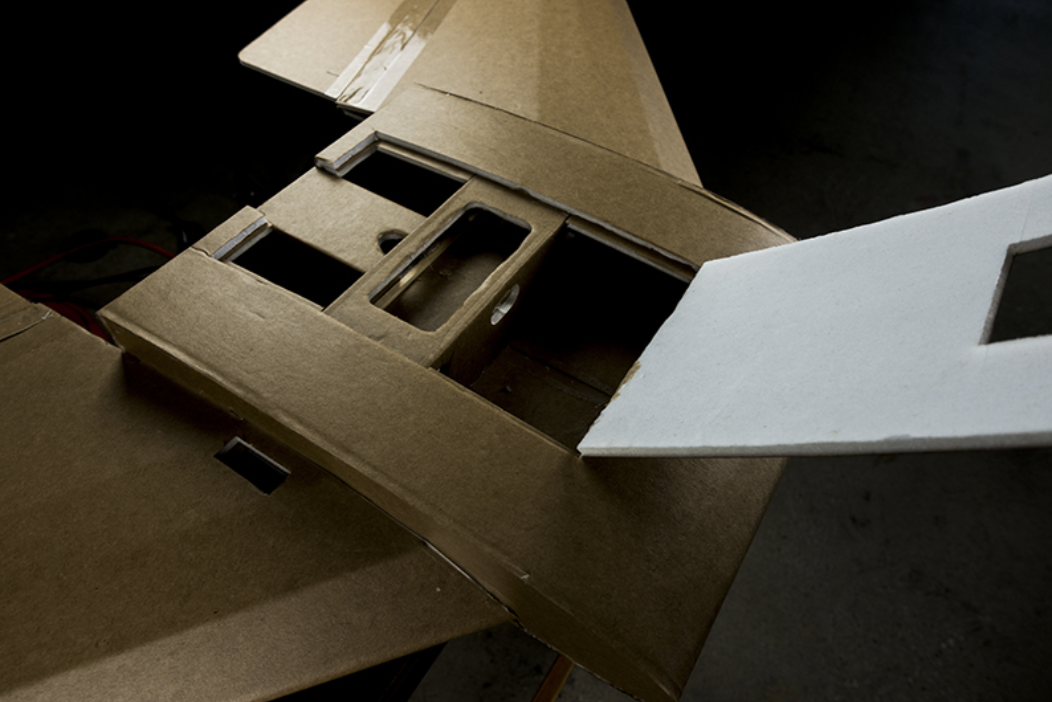
\includegraphics[width=0.6\textwidth]{spear_cargo.png}
  \caption{Spear Cargo Capacity.  Source \cite{flitetest}.}
  \label{fig:spear_cargo}
\end{figure}

This plane was constructed out of craft foam board.  The plans were downloaded from flitetest.com\cite{flitetest} and converted to CorelDraw vector files for use in a laser cutter.  These files were then cut out of four sheets of foam board using the laser cutter.  The wing halves were joined with standard box tape and hot glue.  This provided a cheap and rapid construction process which was achievable under four hours of build time.

\begin{figure}[!h]
 \centering
  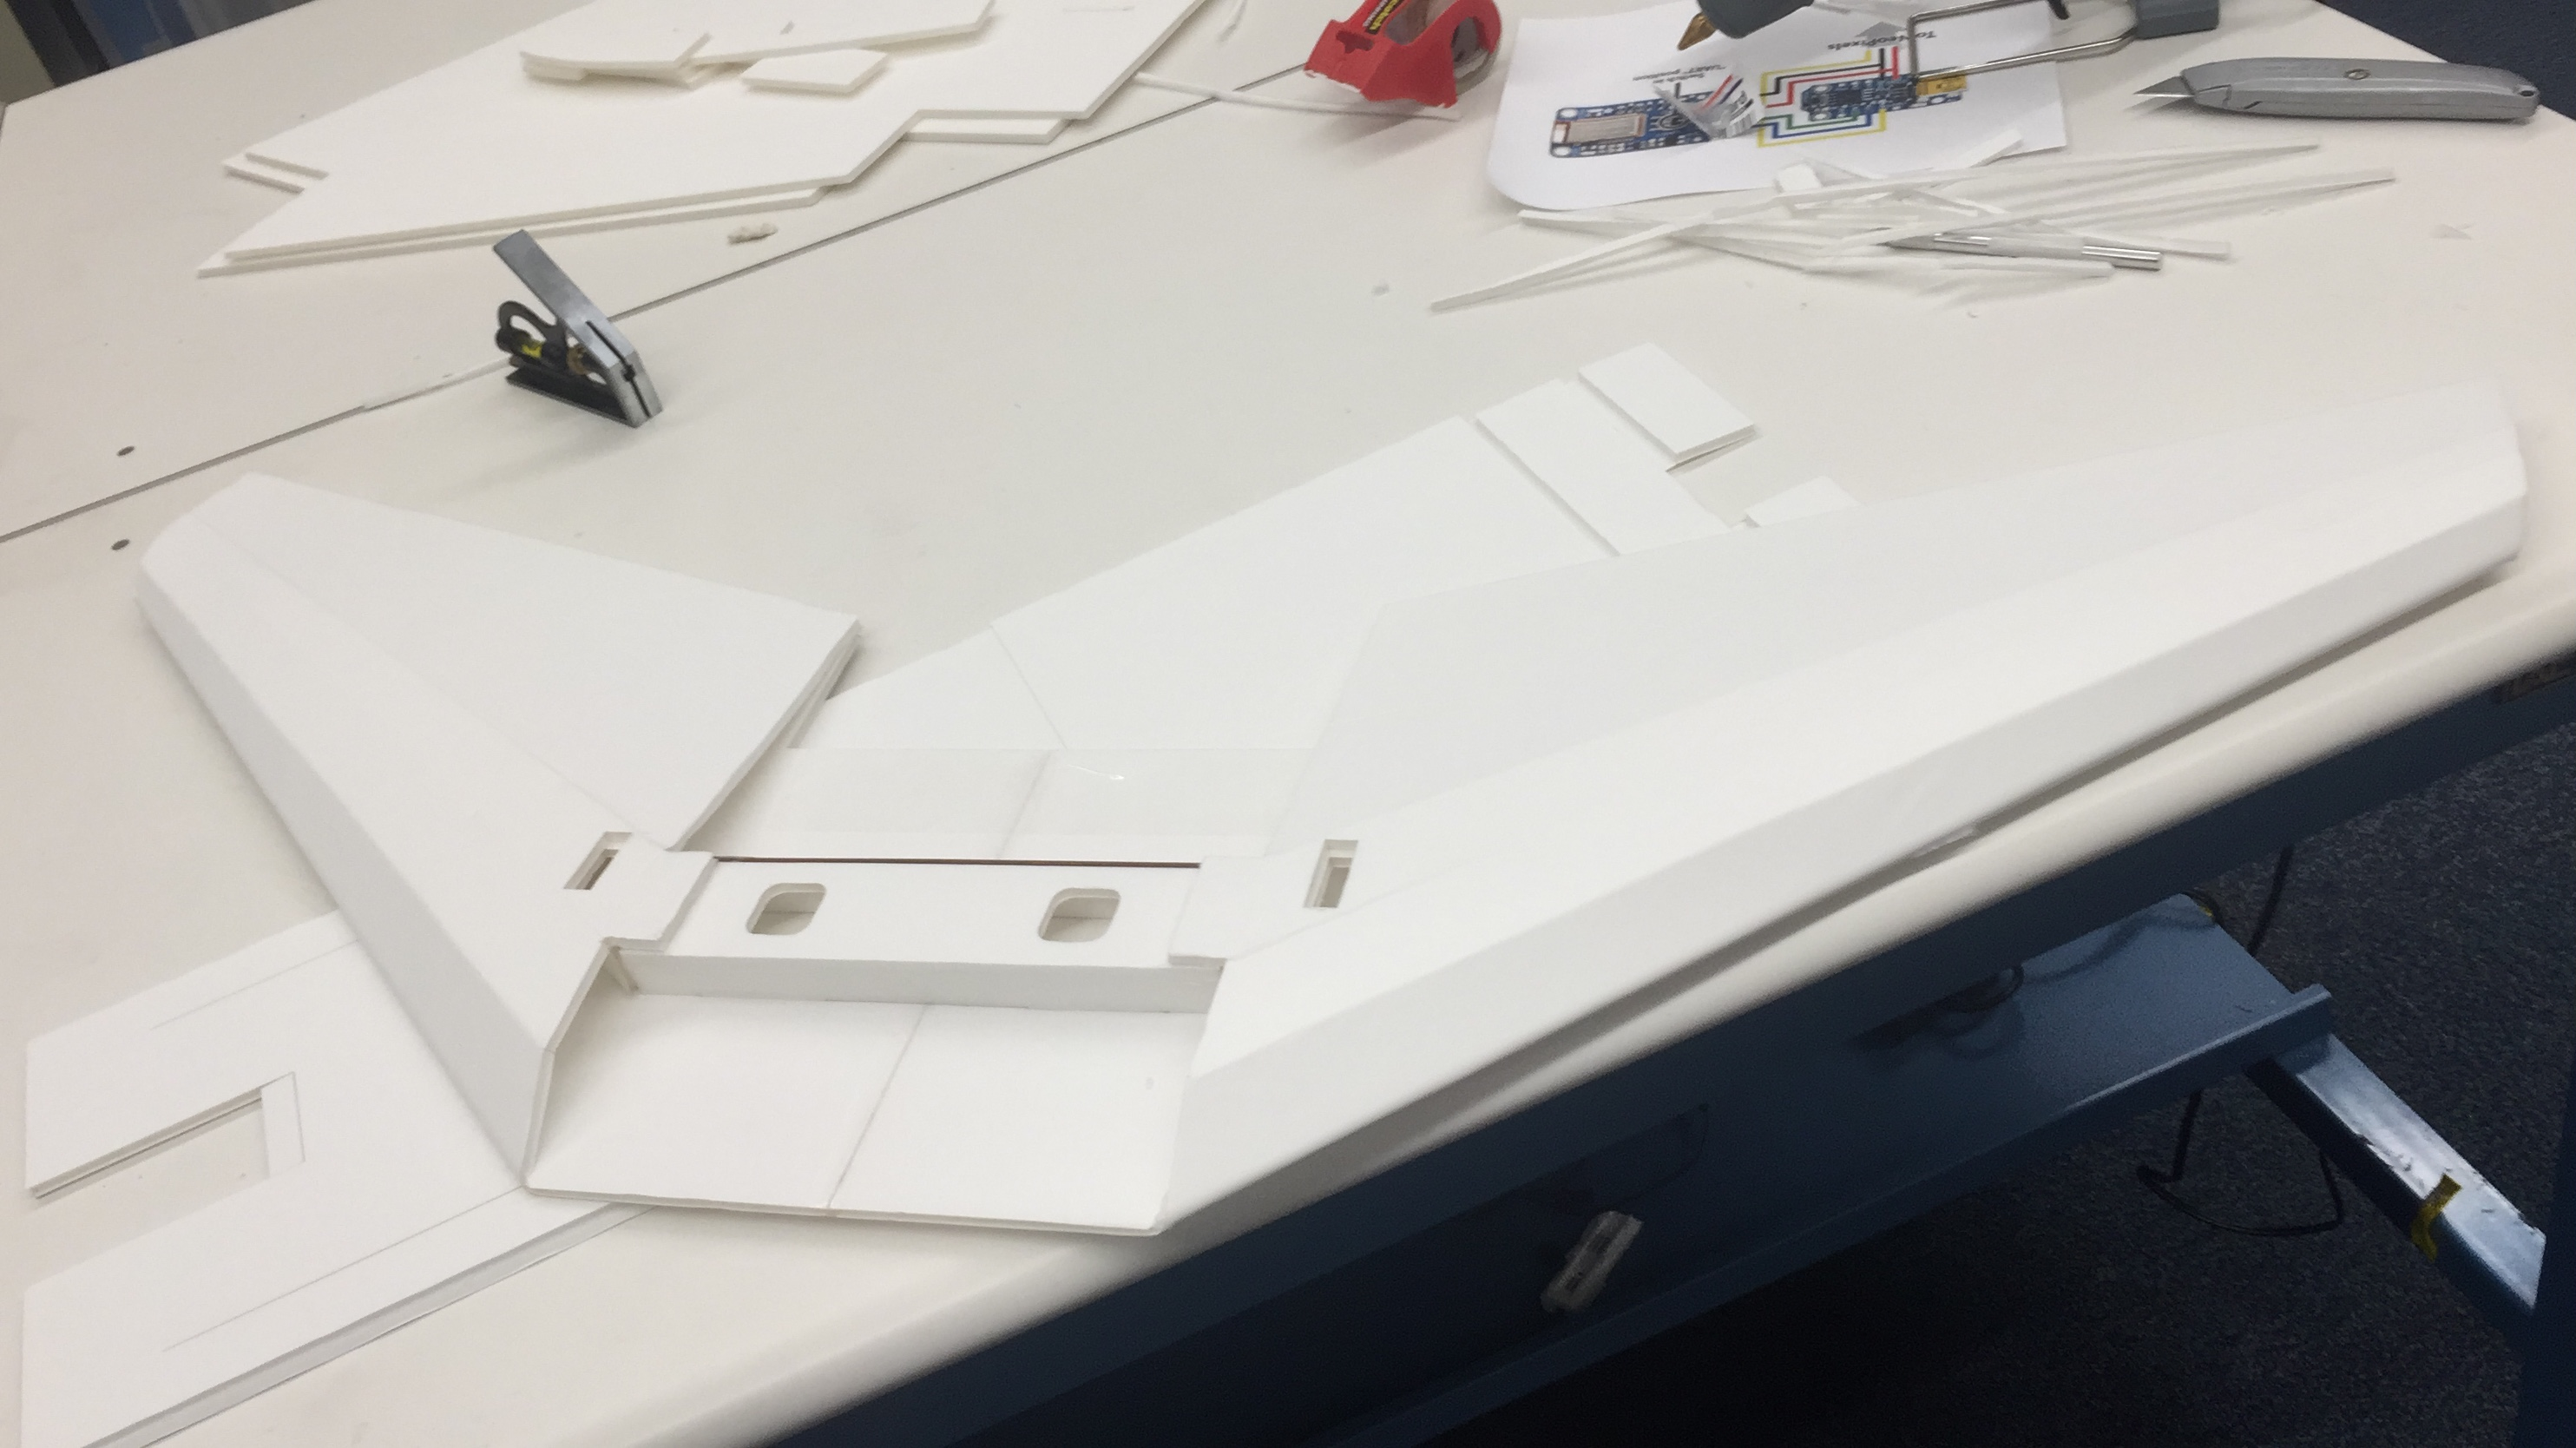
\includegraphics[width=0.6\textwidth]{spear_build.jpg}
  \caption{Spear Build Process}
  \label{fig:spear_build}
\end{figure}

\subsection{Spear Specifications}
\begin{itemize}
 \item weight without battery: 1.45 lbs (658 g)
 \item center of gravity: 3 – 3.5” (76 – 89 mm) in front of firewall
 \item control surface throws: 16\degrees  deflection – Expo 30\%
 \item wingspan: 41 inches (1041 mm)
 \item motor: 425 sized, 1200 kv minimum
 \item prop: 9 x 4.5 CW (reverse) prop
 \item electronic speed control (ESC): 30 amp minimum
 \item battery: (2) 2200 mAH 12.6 volt minimum
 \item servos: (2) 9 gram servos 
\end{itemize}

The Explorer airframe was chosen because it is a conventional airframe with highly coupled aerodynamics which can be configured in multiple different failure modes.  The sport wing provided in the plans was modified to have independently actuated flaps, and ailerons for a combination of software enabled failure modes.  This aircraft was also configured with a rudder for testing the lateral aerodynamics coupling effects on the adaptive controller.  Figure~\ref{fig:explorer} illustrates the completed Explorer airframe used in this research.  Figures~\ref{fig:explorer_parts} and \ref{fig:explorer_electronics} are examples of the Explorer build process and autopilot integration.

\subsection{Explorer Specifications}
\begin{itemize}
 \item weight without battery: 1.08 lbs (493 g)
 \item center of gravity: 2.25” (57 mm) from leading edge of wing
 \item control surface throws: 12\degrees  deflection – Expo 30\%
 \item wingspan: 57 inches (1447 mm)
 \item motor: 425 sized, 1000 kv minimum
 \item prop: 9 x 6 CW (reverse) prop
 \item ESC: 30 amp minimum
 \item battery: (1) 2200 mAH 12.6 volt minimum
 \item servos: (6) 9 gram servos 
\end{itemize}

\begin{figure}[!h]
 \centering
  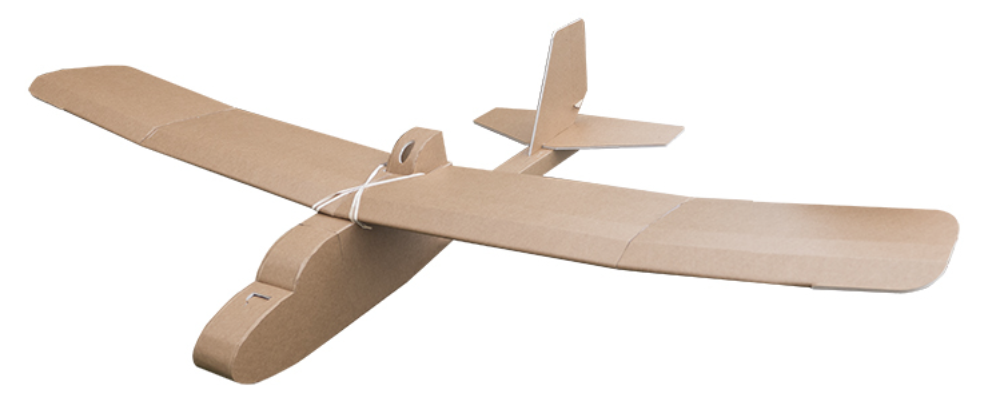
\includegraphics[width=0.90\textwidth]{explorer.png}
  \caption{FliteTest Explorer.  Source \cite{flitetest}.}
  \label{fig:explorer}
\end{figure}

\begin{figure}[!h]
 \centering
  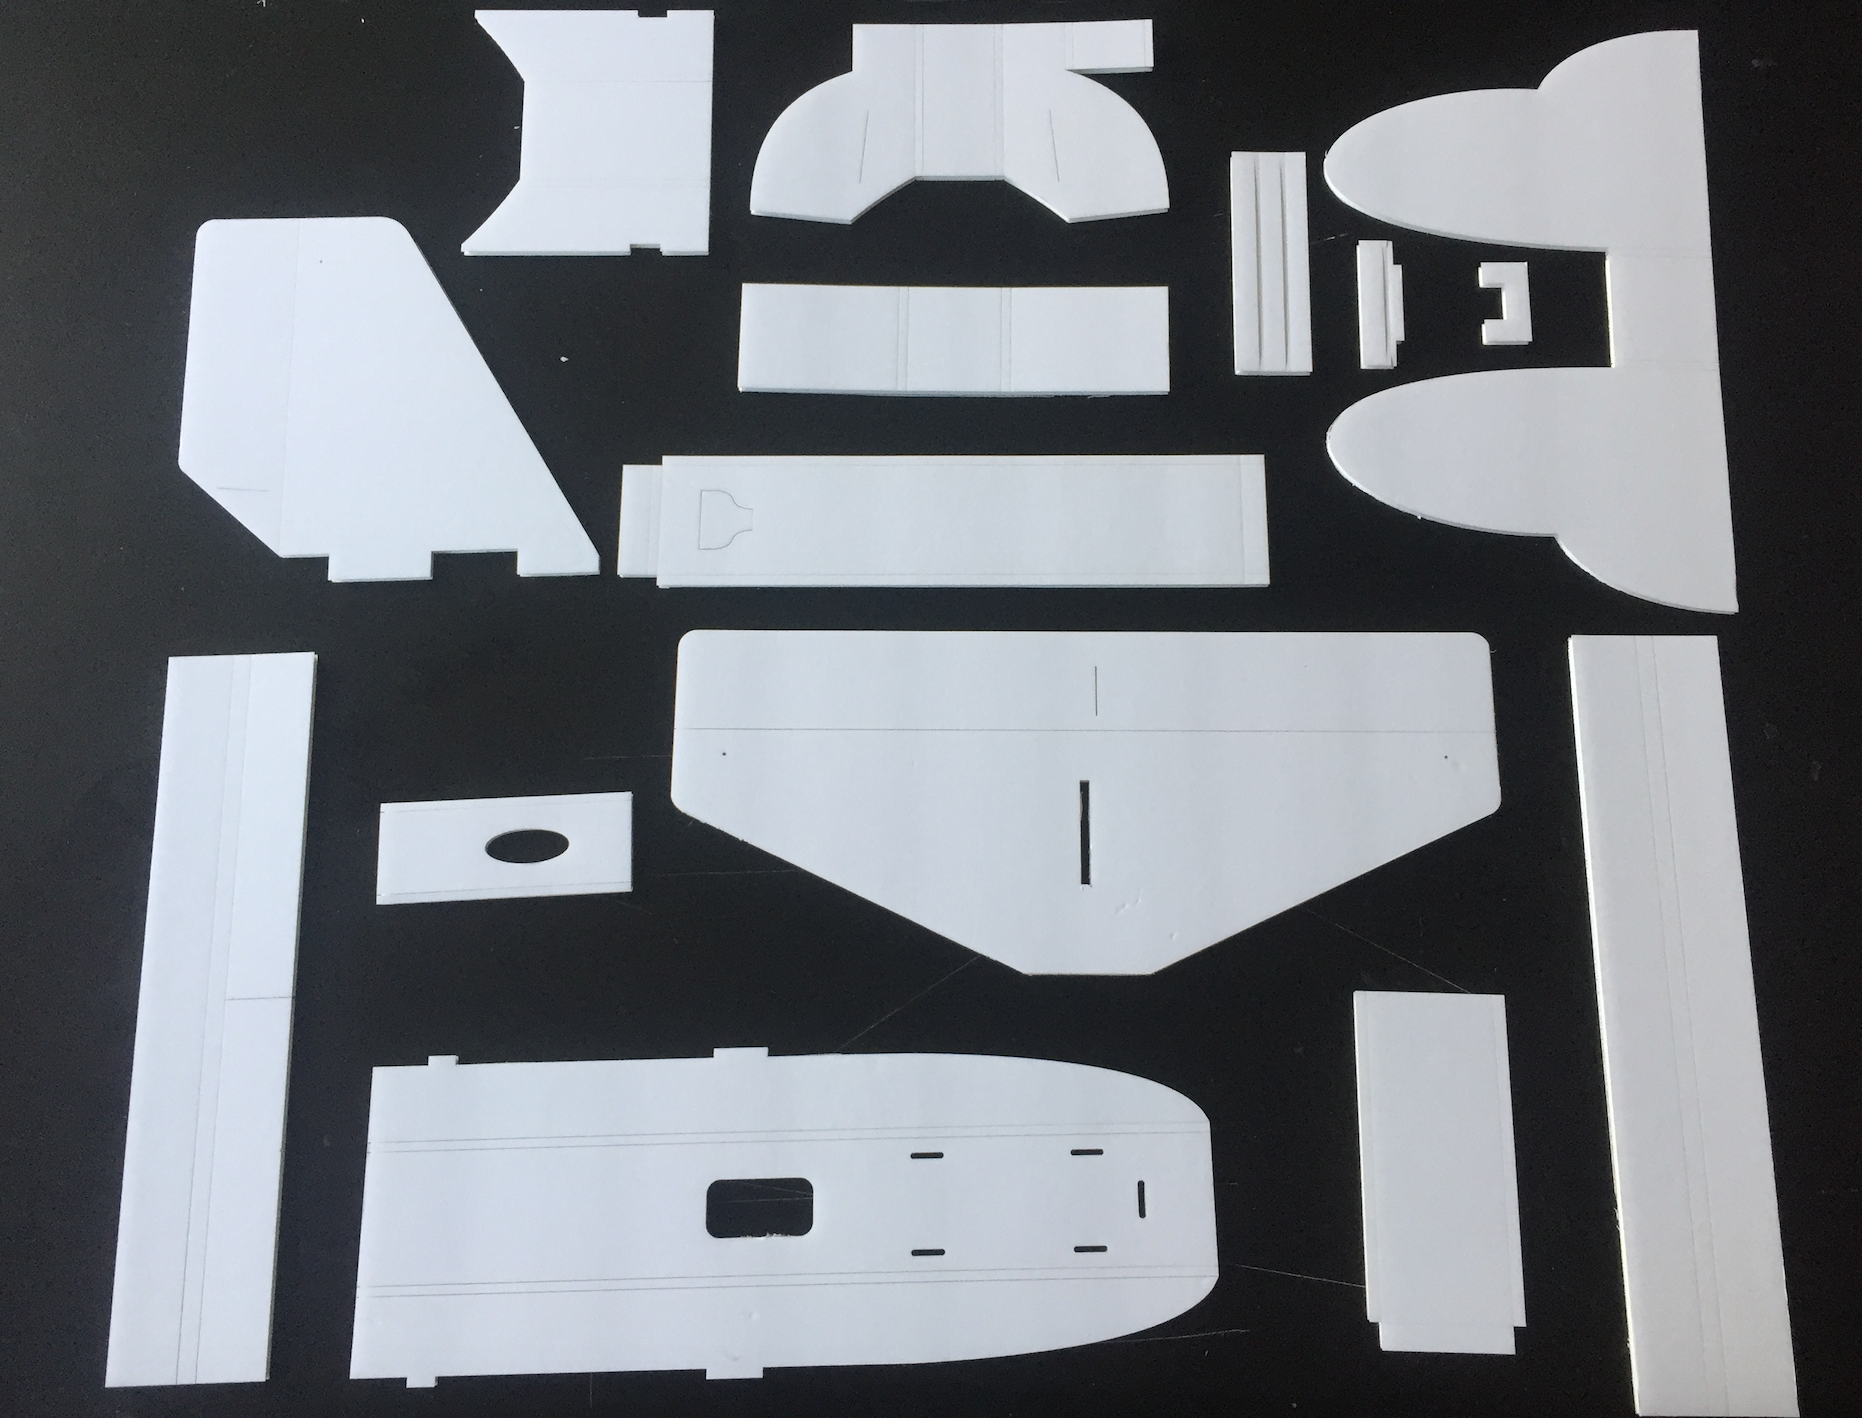
\includegraphics[width=0.85\textwidth]{explorer_parts.png}
  \caption{Explorer Cut Foamboard Parts}
  \label{fig:explorer_parts}
\end{figure}

\begin{figure}[!h]
 \centering
  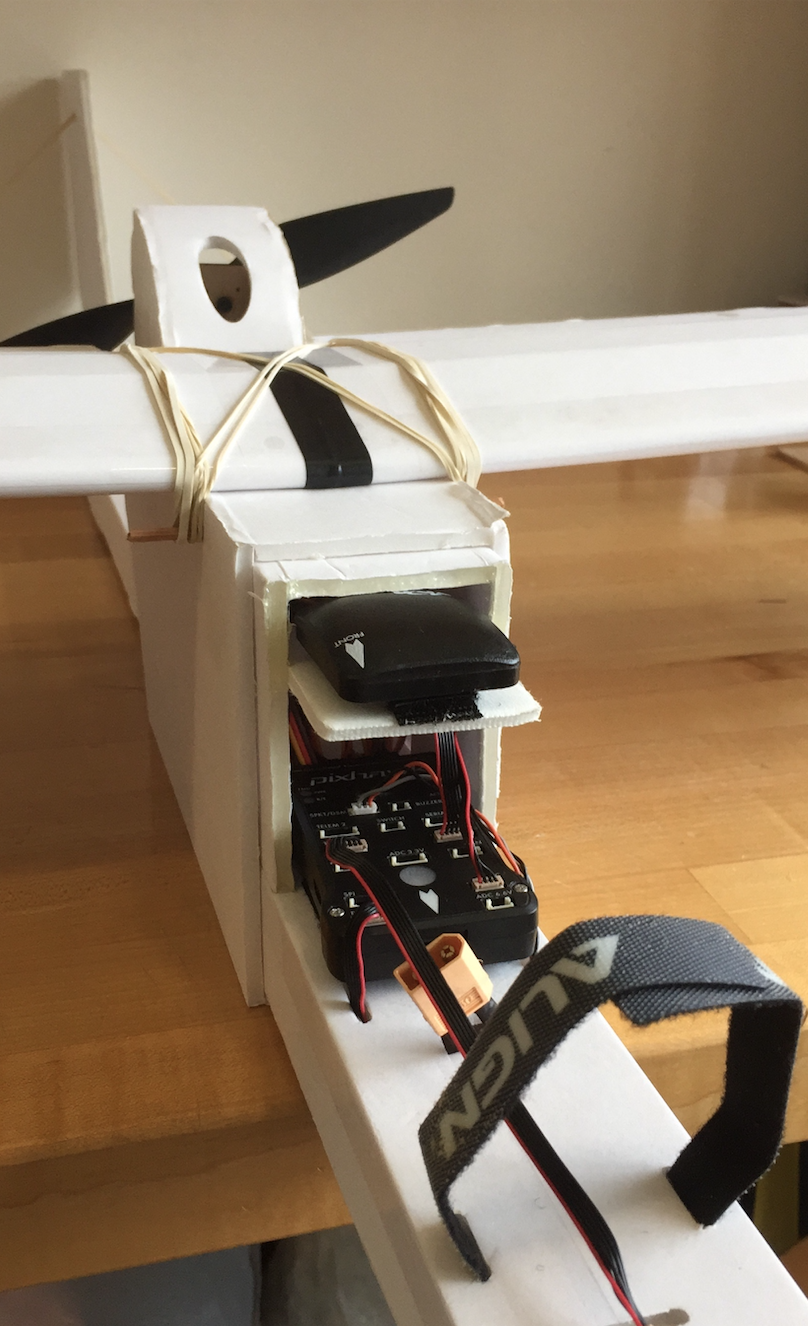
\includegraphics[width=0.75\textwidth]{explorer_electronics.png}
  \caption{Pixhawk Autopilot Installed on Explorer}
  \label{fig:explorer_electronics}
\end{figure}

The previously discussed \ac{COTS} autopilot, Linux software tool chain for \ac{SITL} and \ac{GCS}, and prototype aircraft were utilized to present the results found in Chapter~\ref{ch:performance}.



 	%Design of Experimental Platform
\chapter{Flight Testing and Performance Evaluation}\label{ch:performance}

\section{Simulation Results}
Simulation results were captured utilizing the \ac{APM} \ac{SITL} using X-Plane10.  The aircraft model chosen was an open-source flying wing model called the maxi-swift as seen in figure~\ref{fig:maxi-swift}.

\begin{figure}[!h]
 \centering
  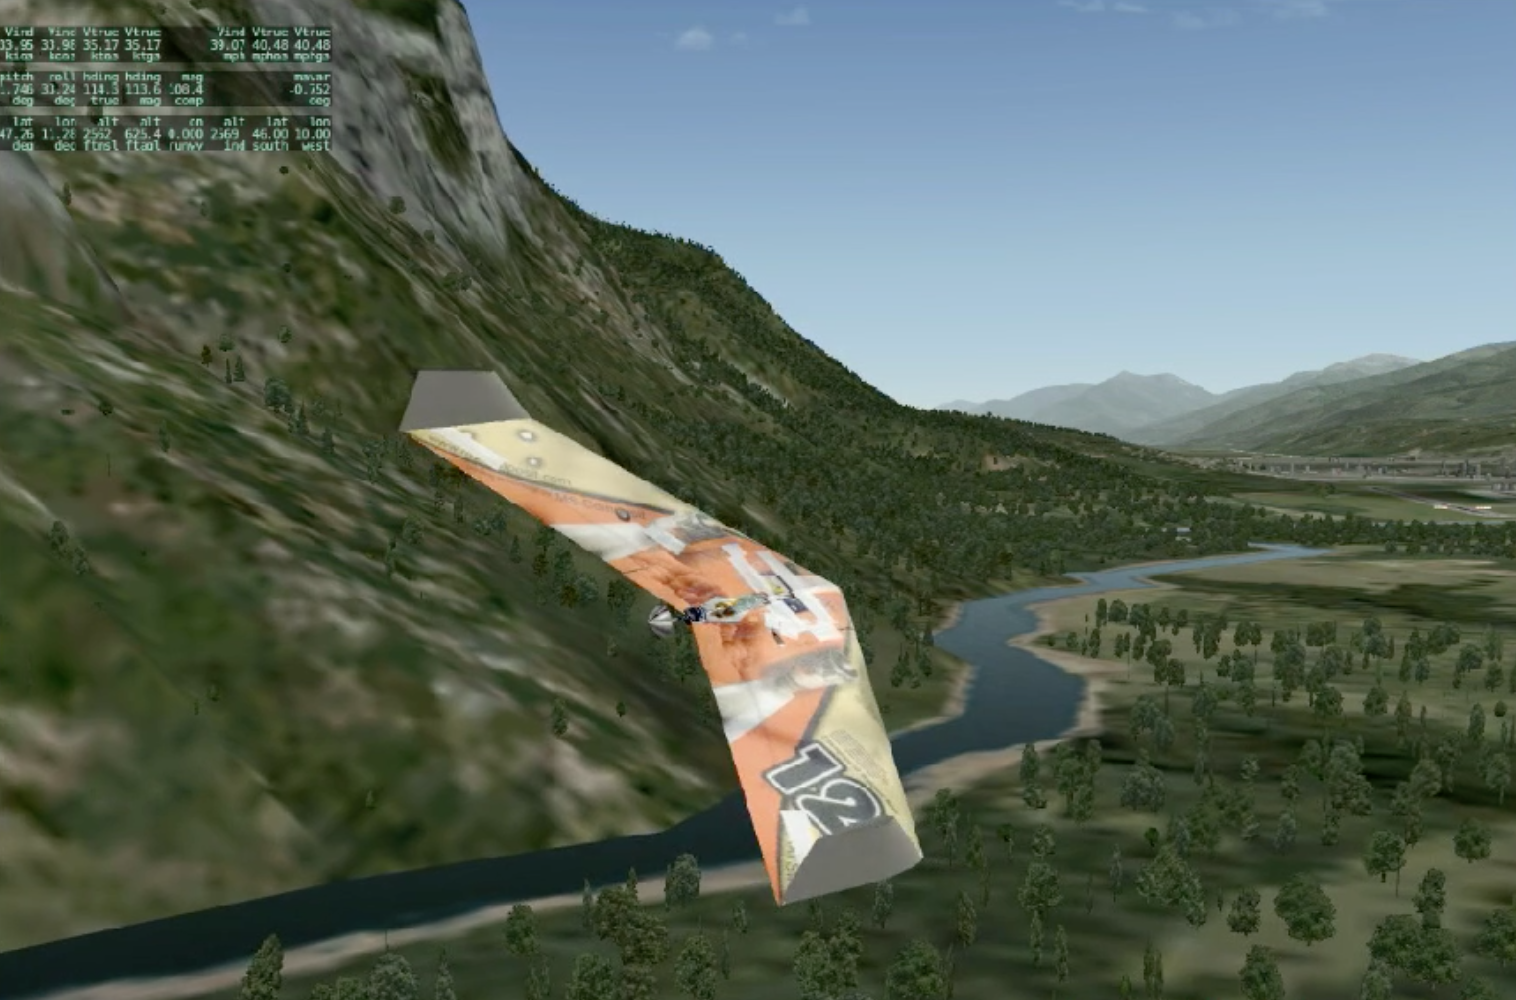
\includegraphics[width=0.75\textwidth]{maxi-swift.png}
  \caption{Maxi-Swift Flying Wing Model used in X-Plane10}
  \label{fig:maxi-swift}
\end{figure}
This plane did not afford proper testing of elevon mixing, but the fidelity in the model provided utilizing X-Plane10 was surprisingly accurate with respect to the FT-Spear aircraft used for actual flight test.  This drastically increased confidence that anything tested in \ac{SITL} would have a high probability of success in actual flight test.


\subsection{Pitch Attitude Performance}

It can be seen in figure~\ref{fig:pitch_perf} that there exists some steady state error when under \ac{PID} control.  This phenomenon is more pronounced when the desired pitch attitude is negative.  This steady state error is due to the increase in lift caused by the increasing airspeed.  The \ac{PID} controller underperforms in this regime.  However, the adaptive controller is able to compensate for these dynamics fast enough to track the desired attitude with no steady state error.

\begin{figure}[h!]
 \centering
  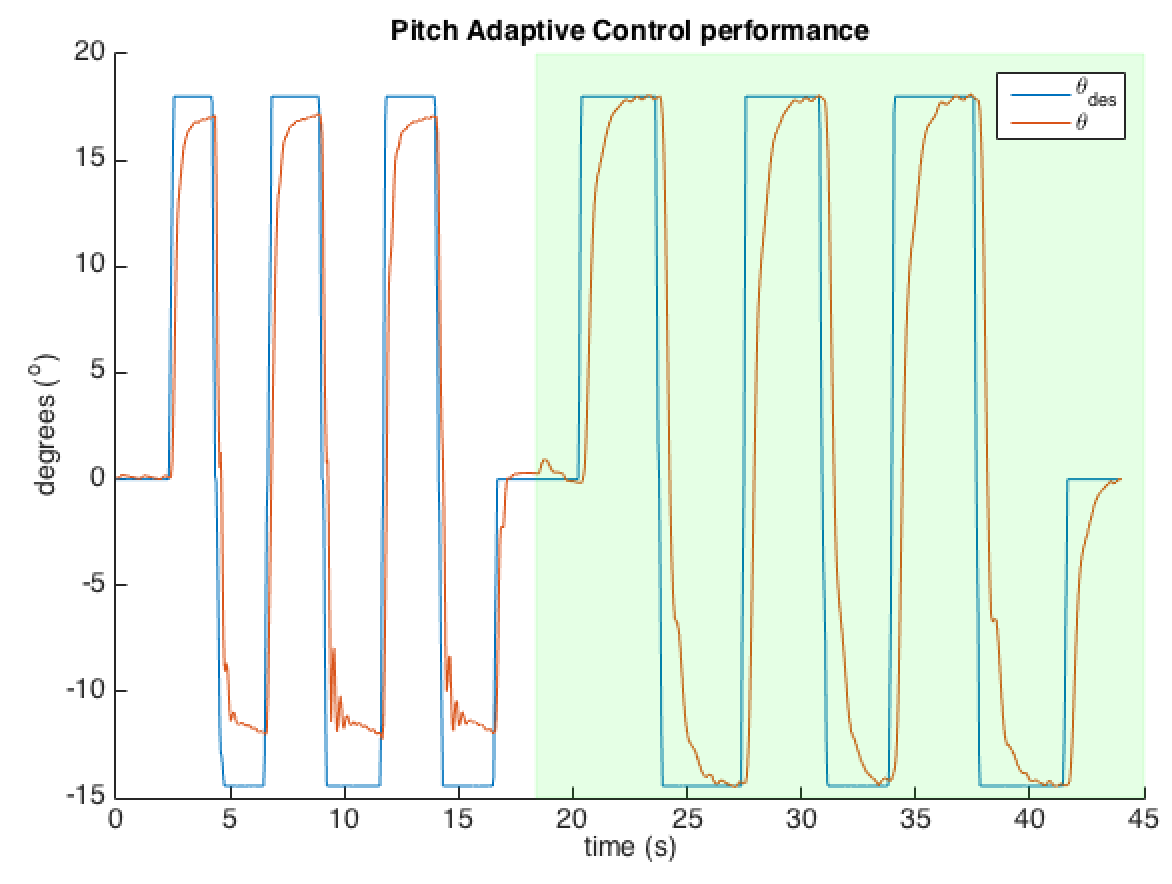
\includegraphics[width=1\textwidth]{pitch_perf.png}
  \caption{PID vs \Lone Adaptive Control Pitch Performance}
  \label{fig:pitch_perf}
\end{figure}

\subsection{Roll Induced Pitch Disturbance}
When rapidly rolling the maxi-swift aircraft in simulation, there was a noticeable coupling in the pitch axis.  The \ac{PID} controller struggles to correct this discrepancy because the time constant of the integral error simply cannot be increased high enough to achieve satisfactory compensation.  As seen in figure~\ref{fig:pitch_divergence}, the \Lone adaptive controller significantly reduced the pitching disturbance due to rapid rolling.

\begin{figure}[h!]
 \centering
  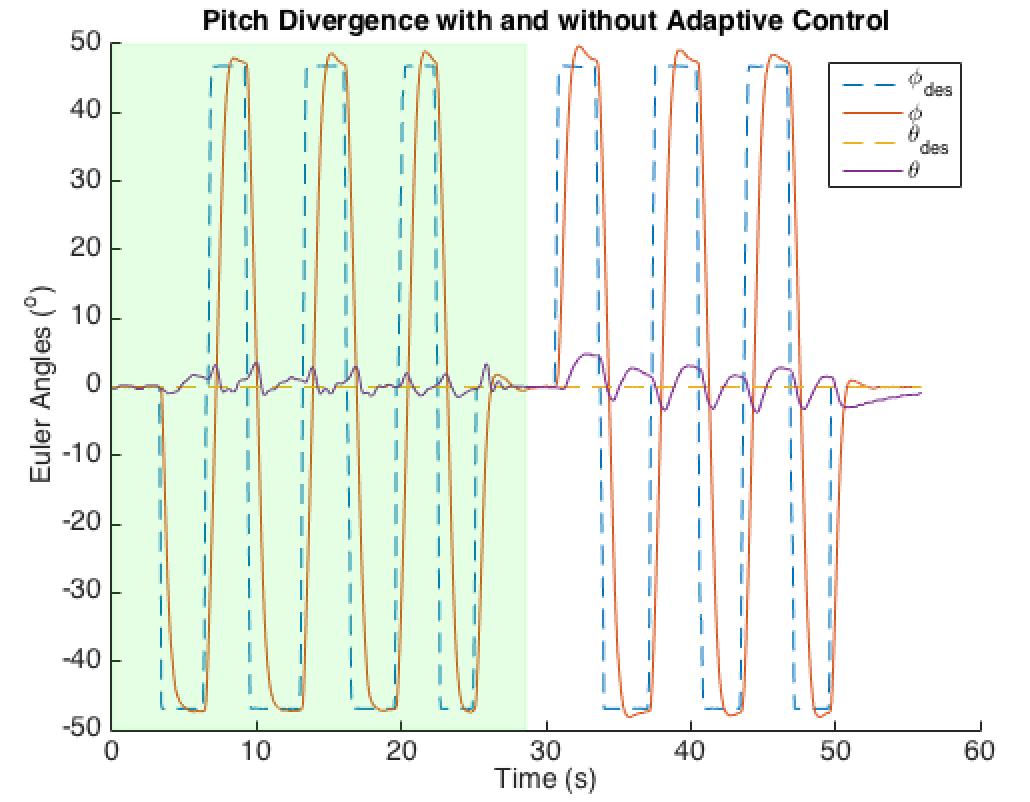
\includegraphics[width=1\textwidth]{pitch_divergence.png}
  \caption{PID vs \Lone Adaptive Control Coupled Pitch Resonse Performance}
  \label{fig:pitch_divergence}
\end{figure}

\subsection{Pitch due to Landing Gear and Flaps}
Lowering the landing gear and flaps entering the landing phase of flight causes un-commanded deviation in pitch.  The F4U Corsair (see figure~\ref{fig:corsair})in X-Plane10 was used to evaluate the attitude hold retention performance.  This un-modeled aerodynamics can cause the integrator in a \ac{PID} controller to saturate or wind up. 

\begin{figure}[h!]
 \centering
  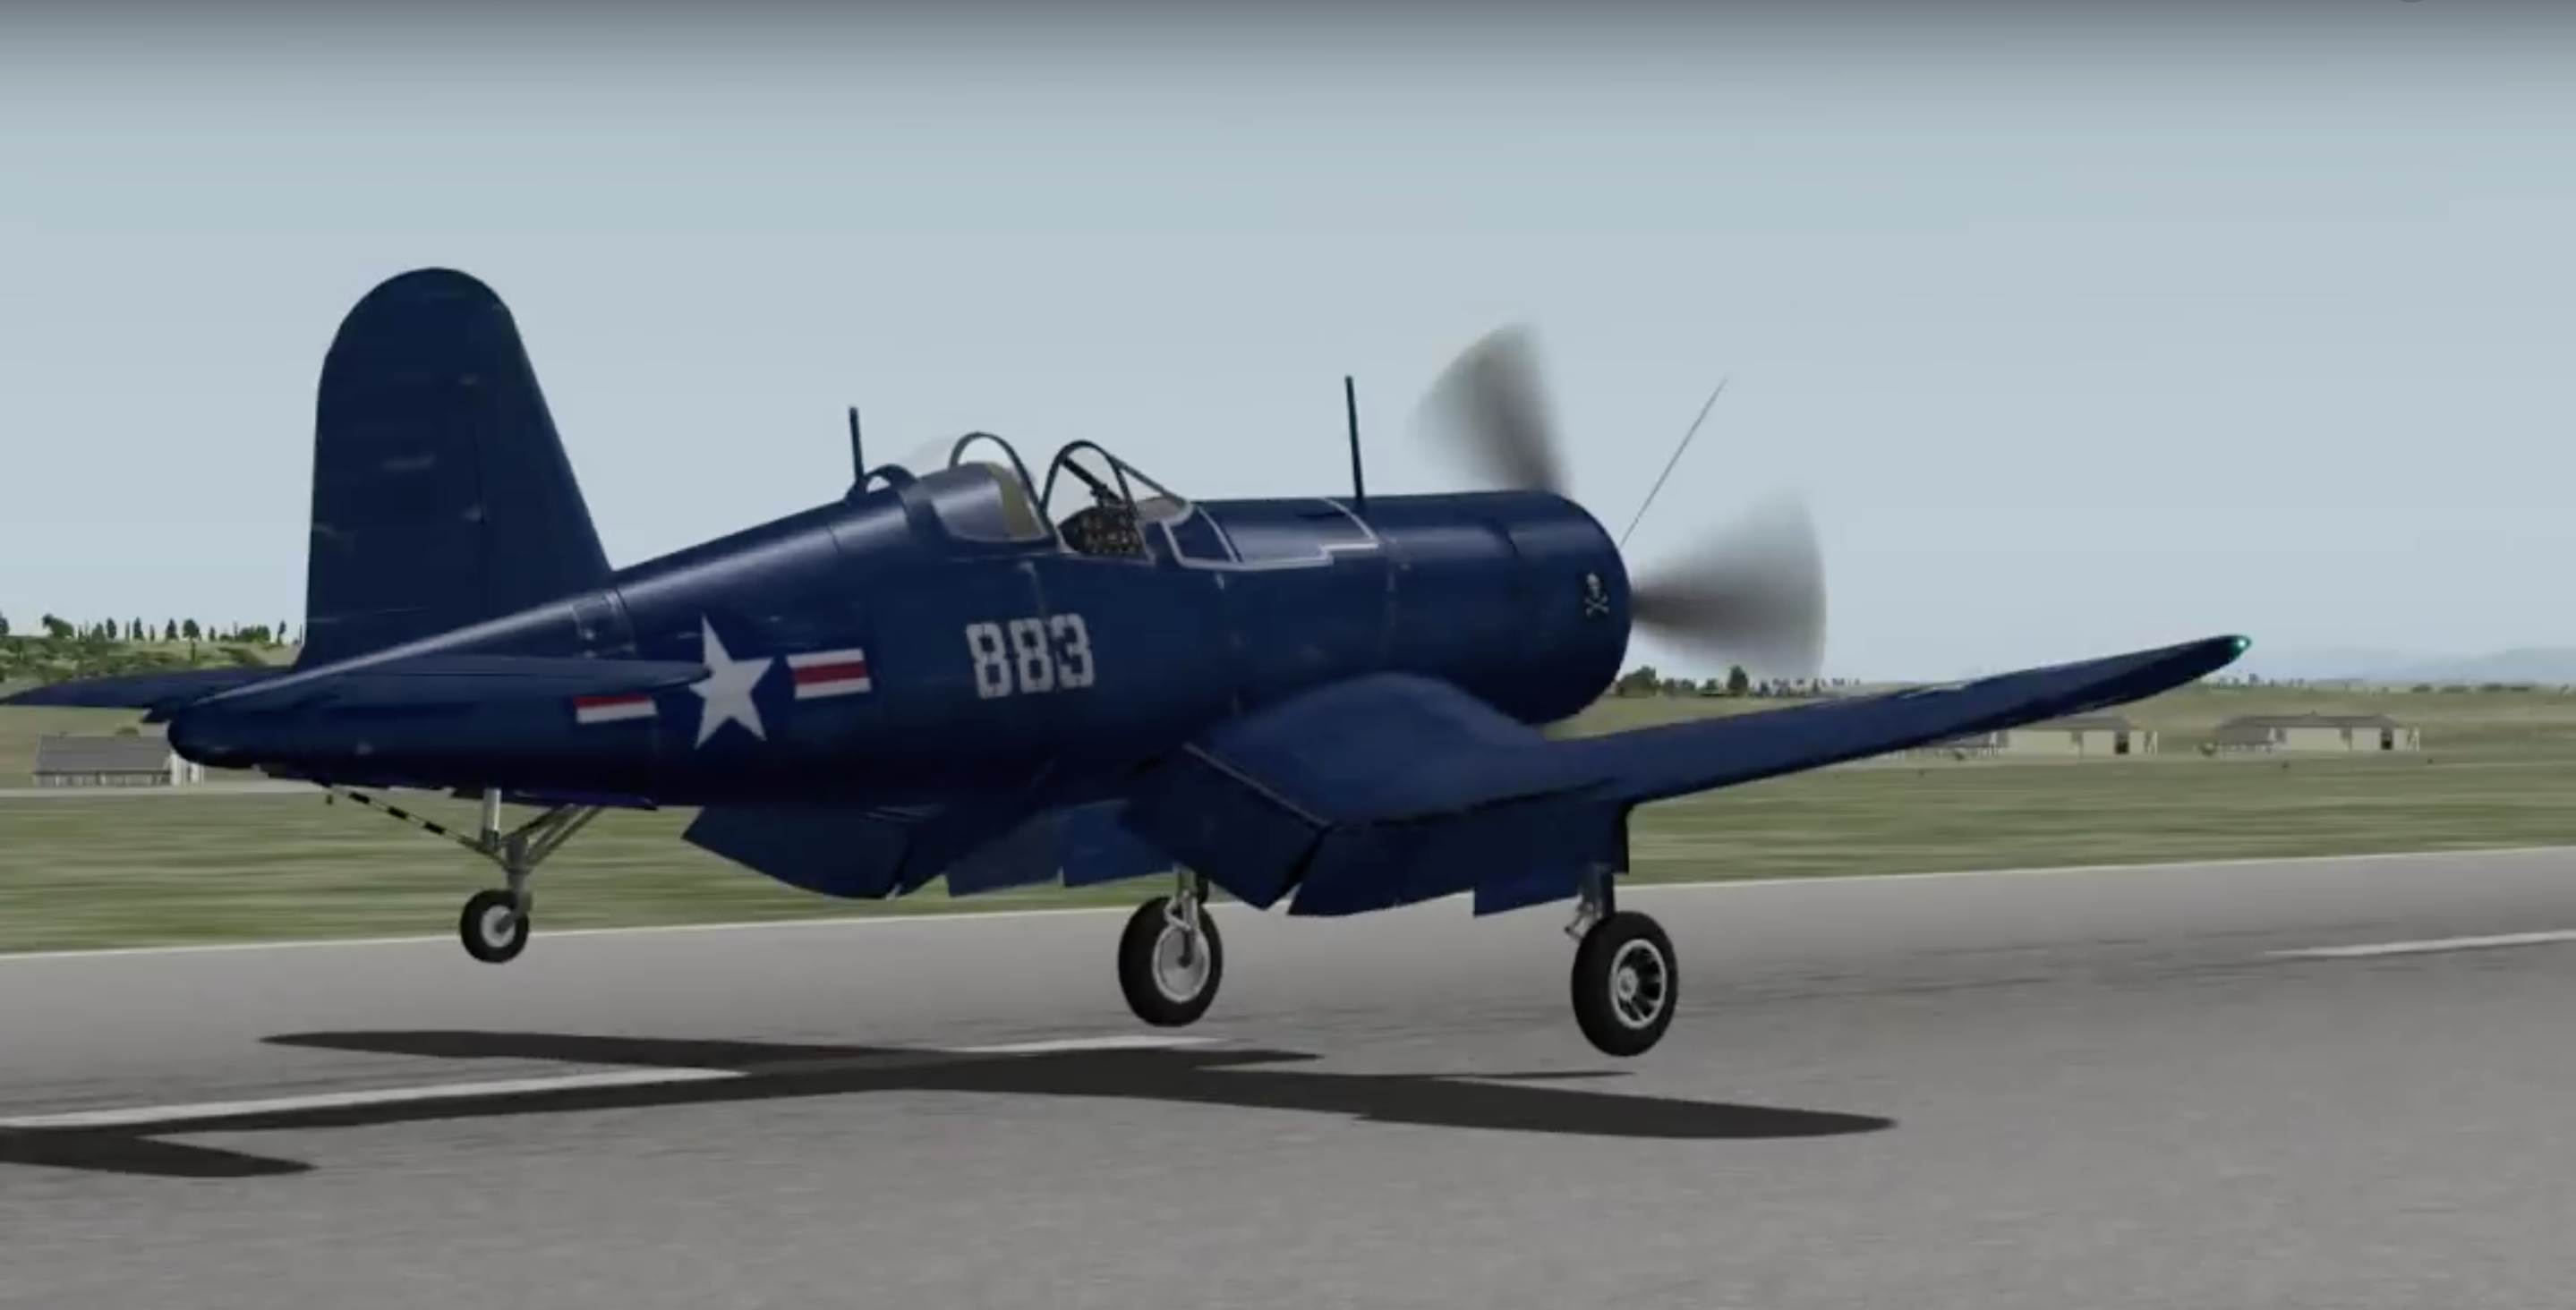
\includegraphics[width=0.85\textwidth]{corsair.png}
  \caption{F4U Corsair model - X-Plane10}
  \label{fig:corsair}
\end{figure}

The \Lone adaptive controller significantly reduces the attitude excursion due to flaps and landing gear.
\begin{figure}[h!]
 \centering
  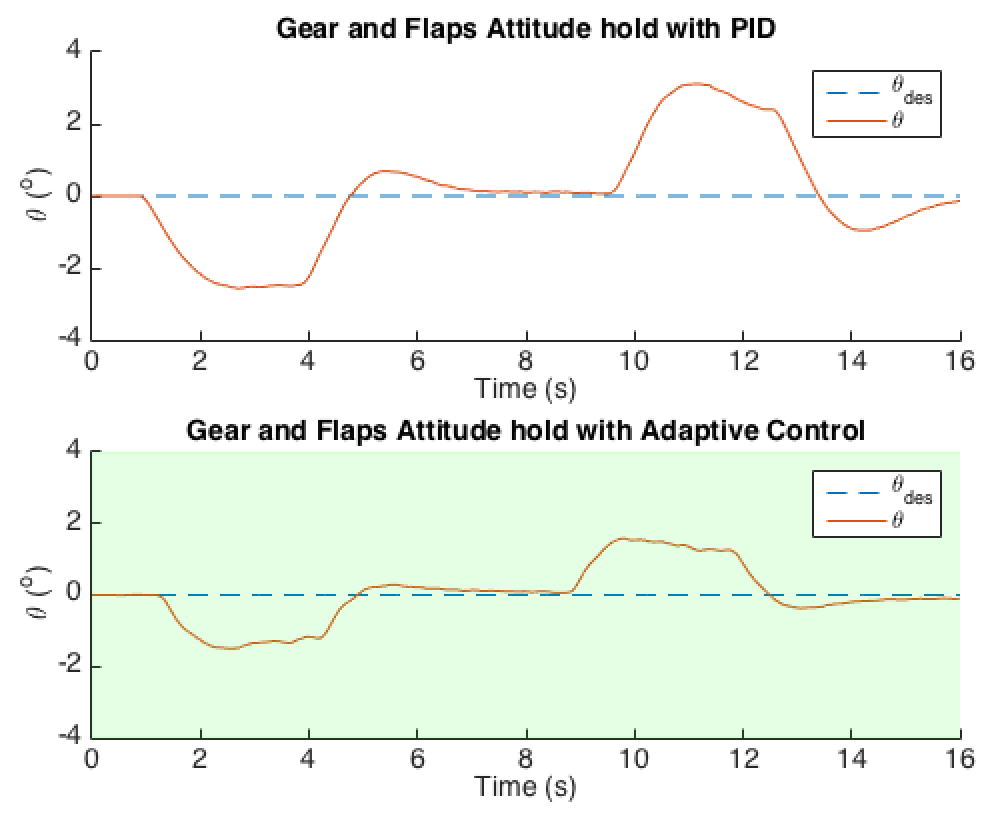
\includegraphics[width=0.85\textwidth]{gear_and_flaps.png}
  \caption{Pitch Attittude Response due to Gear and Flaps}
  \label{fig:gear_and_flaps}
\end{figure}

%---------------------------------------------
\subsection{Roll Performance}
Adaptive control offered little improvement to roll performance with respect to the nominal attitude retention.  The roll axis for multiple aircraft was typically seen to have higher cutoff frequencies with respect to pitch and therefore required higher values for the $D(s)$ cut off frequencies.
\begin{figure}[h!]
 \centering
  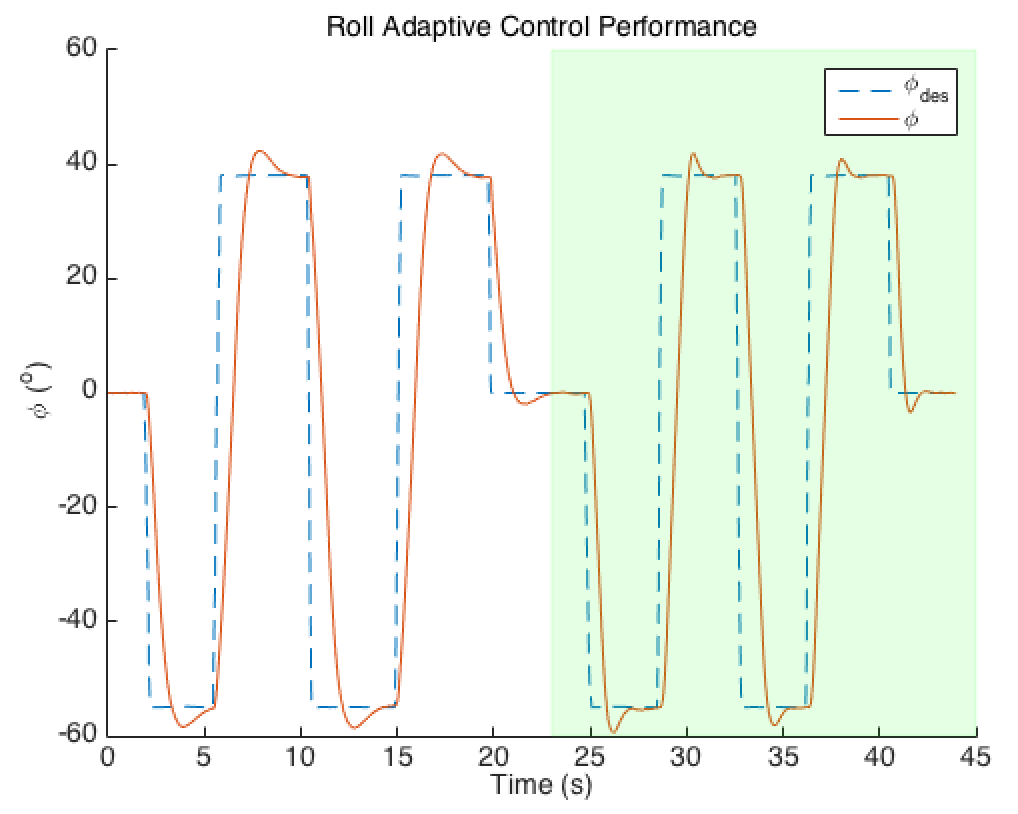
\includegraphics[width=0.85\textwidth]{roll_perf.png}
  \caption{Roll Attittude Performance}
  \label{fig:roll_perf}
\end{figure}

\subsection{Yaw to Roll Coupling}
The roll dynamics are coupled to the yaw dynamics as seen in equation~\ref{eq:aero_torques}.  In the case of an actuator/servo hardover in the yaw channel, the coupling causes unwanted rolling moments.  Figure~\ref{fig:rudder_failure} compares a left and right yaw servo hard over for both \ac{PID} and the \Lone controller.
\begin{figure}[h!]
 \centering
  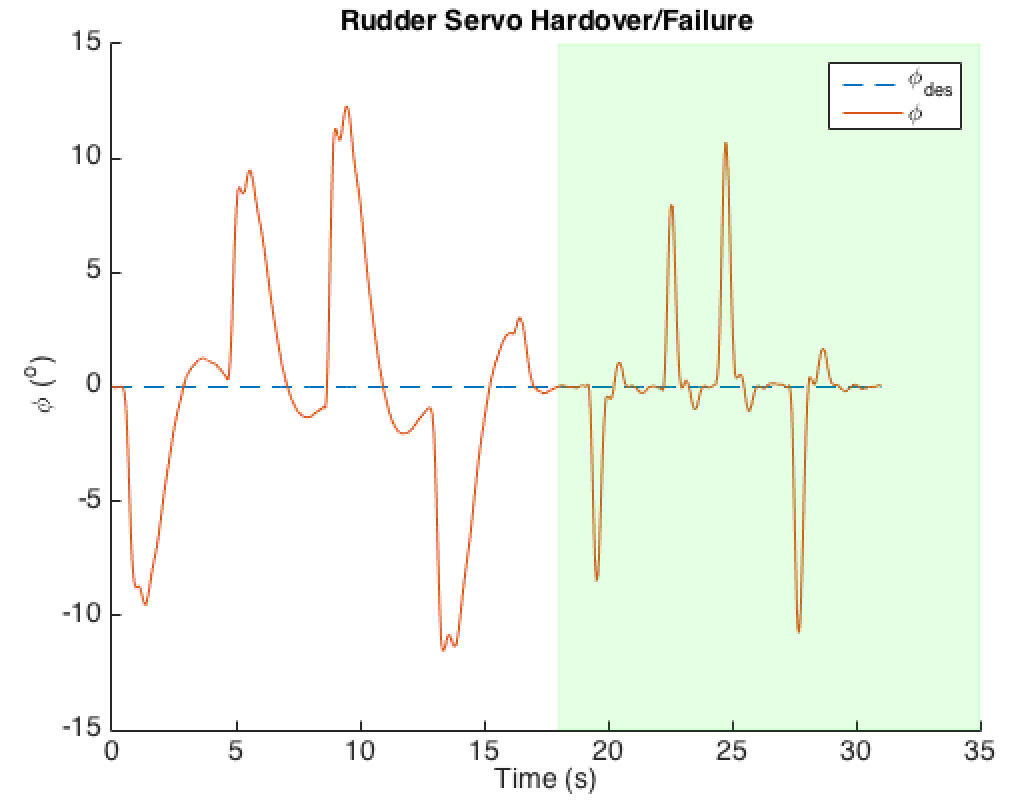
\includegraphics[width=0.85\textwidth]{rudder_failure.png}
  \caption{Roll Response to Rudder Servo Hardover/Failure}
  \label{fig:rudder_failure}
\end{figure}
The adaptive controller significantly outperforms the \ac{PID} controller in maintaining the desired roll.  It could be argued that the \ac{PID} controller's integrator time constant could be re-tuned to be comparable.  It was evident for each of the simulation tests that tuning the \ac{PID} for every scenario would likely have been possible individually to achieve similar performance to the \Lone.  However, the \Lone was not tuned between each of these tests and outperformed \ac{PID} in most, if not all cases.

\subsection{Actuator Miscalibration}
The \Lone adaptive control provided fast learning of airframe actuator miscalibrations.  The autopilot parameter SERVOX\_TRIM was used to offset the ailerons by 15\% of their travel to evaluate how quickly the controller was capable of adapting to the new offset.  This was tested first on the \ac{PID} controller and then on the \Lone as seen in figure~\ref{fig:trim_learn}.
\begin{figure}[h!]
 \centering
  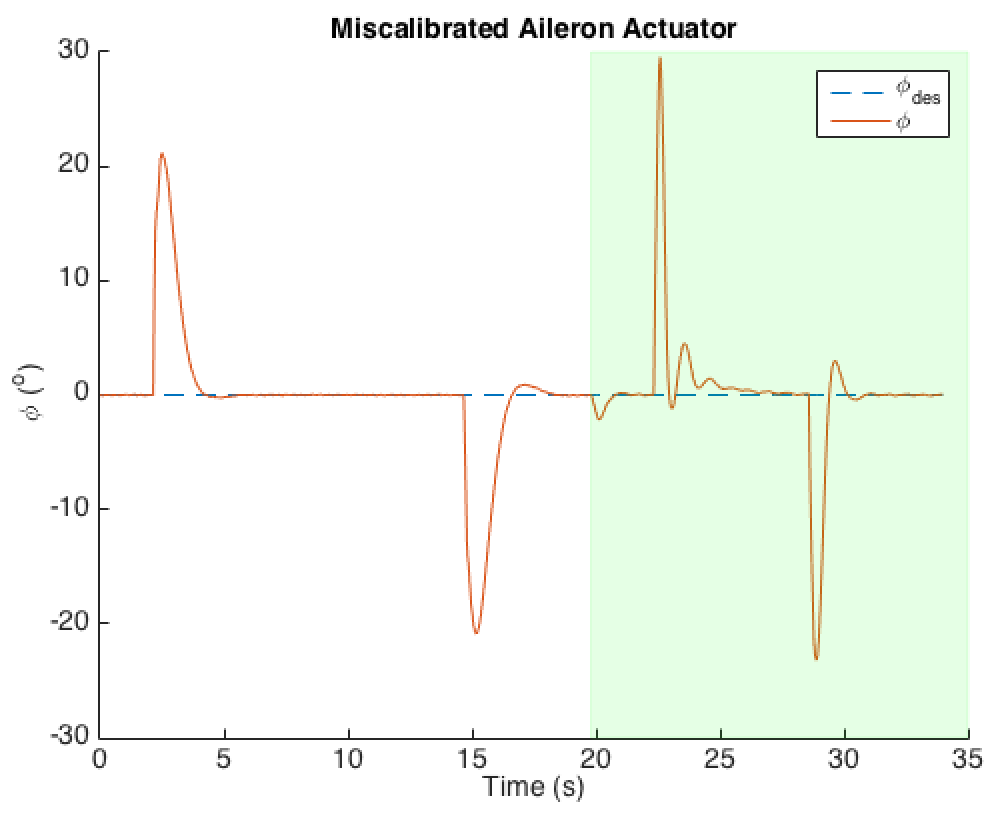
\includegraphics[width=0.65\textwidth]{trim_learn.png}
  \caption{Roll Response to Miscalibrated Aileron Servo}
  \label{fig:trim_learn}
\end{figure}
\begin{figure}[h!]
 \centering
  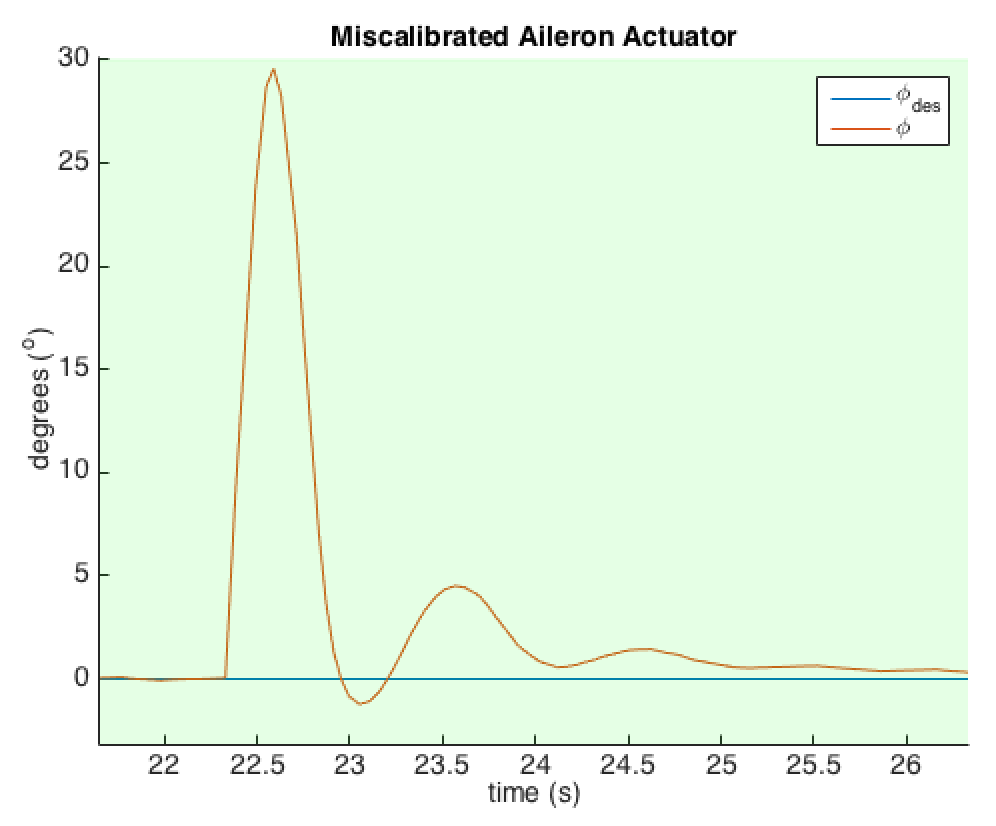
\includegraphics[width=0.65\textwidth]{trim_learn2.png}
  \caption{\Lone Fast Adaptation to Unknown Miscalibration}
  \label{fig:trim_learn2}
\end{figure}

It can be seen in figure~\ref{fig:trim_learn} and \ref{fig:trim_learn2} that the new trim value achieves the reference command in about 0.5 seconds for the \Lone.  The \Lone is slightly faster than \ac{PID}, but the \Lone exhibits some overshoot.  It is important to note that this rate of learning is perfectly adequate for learning the miscalibrations in flight, but is insufficient for learning on take off.  In the takeoff circumstance, the algorithm saturates the actuator if biases exist between desired and achieved.  Because the aircraft has no dynamic pressure (it is not flying), the desired cannot be achieved.  This causes controller saturation, which cannot be unwound fast enough for take-off (specifically for tail-dragger configuration).  This has to be handled with ad-hoc heuristics very delicately.  One could choose to speed scale the learned parameters to help with learning rate, but it was not chosen for this research because this controller is also utilized in tail-sitter configurations where the zero airspeed would cause the controller to refuse to learn when in \ac{VTOL} mode.

%---------------------------------------------
\section{Flight Test Results}\label{sec:flight_test}
\subsection{General Observations}
The FT Spear aircraft was used in all initial flight tests to prove the algorithm's initial robustness and facilitate testing of various tuning scenarios.  Choosing this aircraft proved to be beneficial because it provided 30 or more minutes of endurance.  The flying wing architecture had a slight forward \ac{CG} when configured with two 2200 \ac{mAh} batteries.  This resulted in the aircraft being anemic in pitch response but still adequate for testing the \Lone algorithm.  Various iterations of the algorithm were tested and compared to the results observed in \ac{SITL} as the development progressed.  

The first observation was that the algorithm, even when poorly tuned, was bounded in response and never approached instability.  The gains found in \ac{SITL} when applied to actual flight test always resulted in stable flight.  As discussed in Section~\ref{sec:tuning}, the first flight tests of gains found in \ac{SITL} either produced low-frequency oscillations or high-frequency oscillations.  Low-frequency oscillations occurred when the \Lone filter cutoff bandwidth was set too low.  High-frequency oscillations occurred when the \Lone filter cutoff bandwidth was set too high.  Tuning the filter to achieve adequate response somewhere between the low and high-frequency oscillations was easily achievable within three to four iterations of setting the filter cutoff frequency.  Finding the optimal filter setting is arguably difficult to see on the low refresh rate telemetry, but achieving similar or better performance than \ac{PID} was easily attained with very minimal effort.

Once the algorithm was well understood and properly implemented in code, flight tests were then conducted on the FT Explorer aircraft.  This aircraft provided more test opportunities because multiple aircraft configurations could be tested with various combinations of flaps and rudder.  

\subsection{Pitch Performance}
As demonstrated in figure~\ref{fig:pitch_perf}, the simulation results almost identically matched the flight test results for pitch response.  As the aircraft pitches down, the airspeed builds and causes a building steady state error that the integrator time constant struggles to out pace.  This was observed both in simulation and in flight test.  The \Lone adaptive controller's fast adaptation was sufficient to counteract this unmodeled pitching moment.  These results drastically increased the confidence both in the \ac{SITL} fidelity as well as the \Lone adaptive controller.
\begin{figure}[h!]
 \centering
  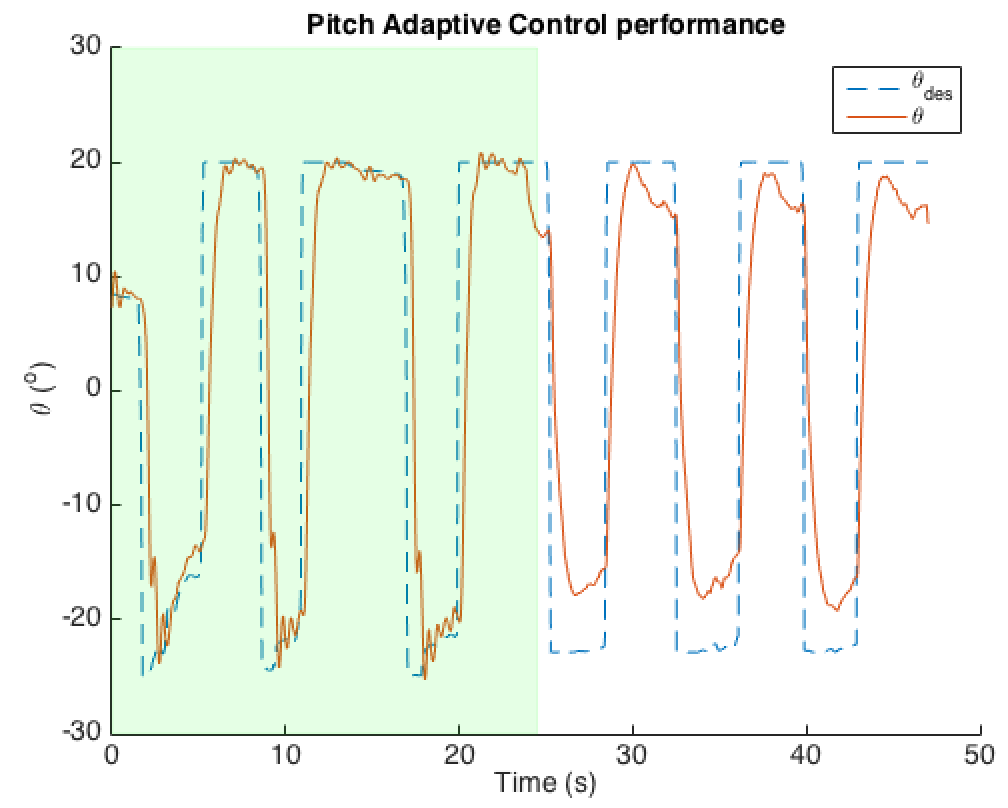
\includegraphics[width=1\textwidth]{pitch_perf_flight_test.png}
  \caption{PID vs \Lone Adaptive Control Pitch Performance}
  \label{fig:pitch_perf_flight_test}
\end{figure}

\subsection{Pitch due to Landing Gear and Flaps}
The \Lone adaptive controller performed well when compensating for the change in aircraft configuration when lowering the flaps.  Figure~\ref{fig:flaps_flight_test} illustrates that the tracking error from lowering and raising the flaps under adaptive control is almost imperceptible.  However, \ac{PID} resulted in a sharp peak both when lowering and raising the flaps.
\begin{figure}[h!]
 \centering
  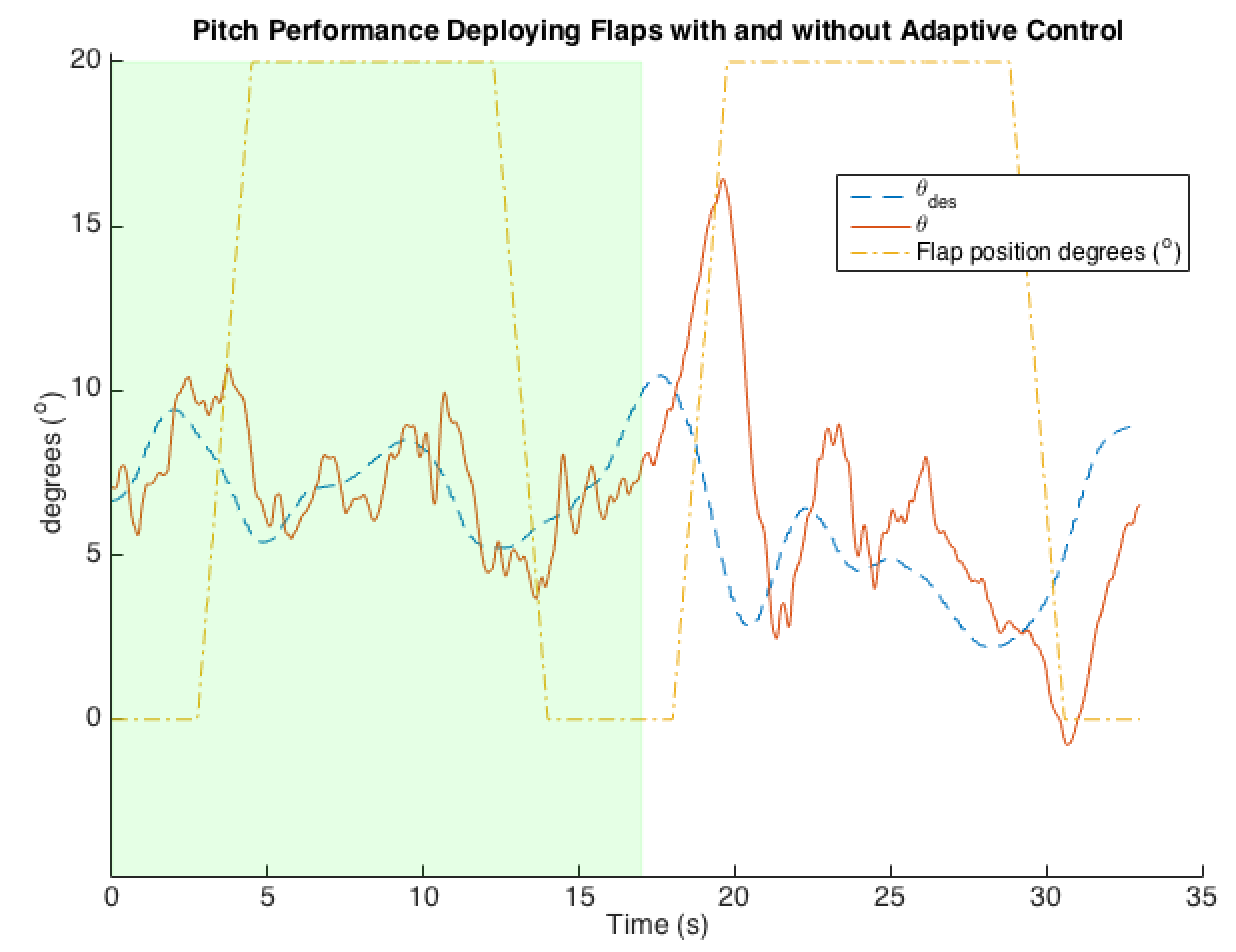
\includegraphics[width=1\textwidth]{flaps_flight_test.png}
  \caption{Pitch Attittude Response due to Gear and Flaps}
  \label{fig:flaps_flight_test}
\end{figure}

\subsection{Roll Induced Pitch Disturbance}
The aircraft max roll angle was set to \pm 45\degrees to achieve rapid roll while trying to maintain a zero pitch attitude.  This rapid roll maneuver caused significant excursions in pitch when under \ac{PID}.  However, the \Lone controller maintains the pitch attitude within \pm 3\degrees.  It can be noticed in figure~\ref{fig:pitch_divergence_flight}, that the adaptive controller oscillates around zero pitch attitude, while the \ac{PID} has more random excursions.  The slight sinusoidal behavior or the \Lone controller is likely due to the cutoff frequency of the filter being slightly too low.  This maneuver may possibly be utilized to fine tune the \Lone's filter cutoff frequency for pitch.
\begin{figure}[h!]
 \centering
  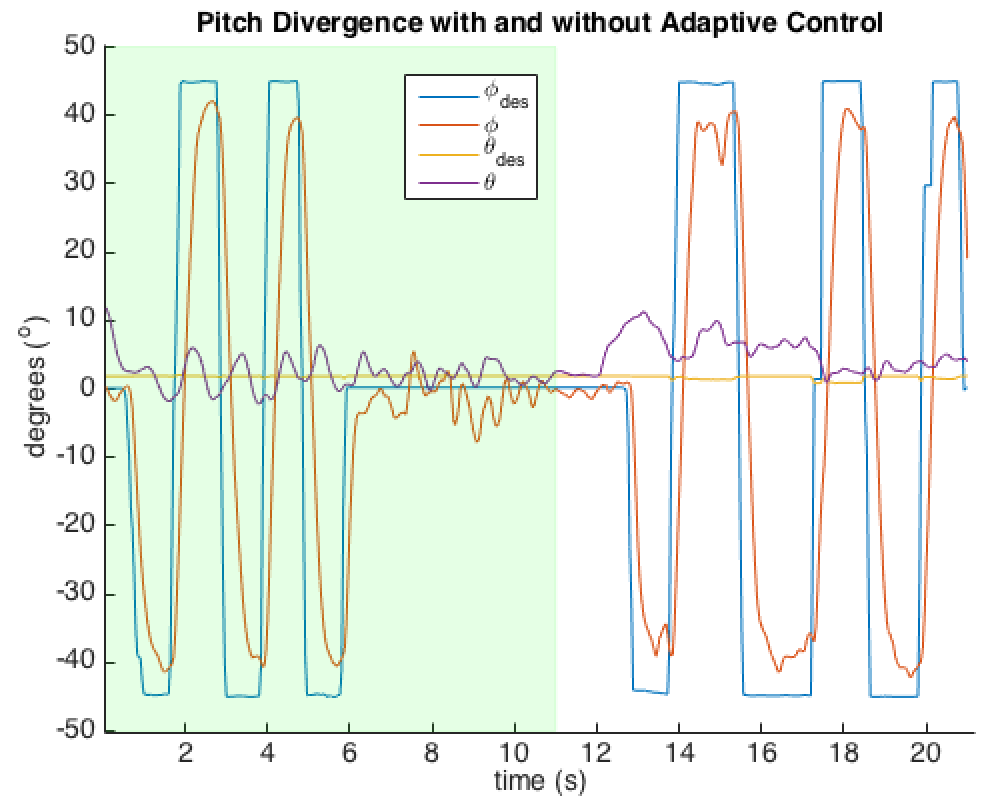
\includegraphics[width=1\textwidth]{pitch_divergence_flight.png}
  \caption{PID vs \Lone Adaptive Control Coupled Pitch Resonse Performance}
  \label{fig:pitch_divergence_flight}
\end{figure}

%---------------------------------------------
\subsection{Roll Performance}
A rectangular flight plan was established to test the nominal flight path stability and roll attitude performance.  Figure~\ref{fig:roll_perf_flight_test} illustrates the \Lone adaptive controller while maintaining the left hand pattern.  The noise in the roll channel was observed in actual flight as turbulence.  The fliter cutoff frequency could be lowered to reduce performance if desired, but these results were not oscillatory which suggested that the filter cutoff frequency was not too high.  These results compare to the noise found on the \ac{PID} channel so the threat of damaging servo by over driving them was not expected.
\begin{figure}[h!]
 \centering
  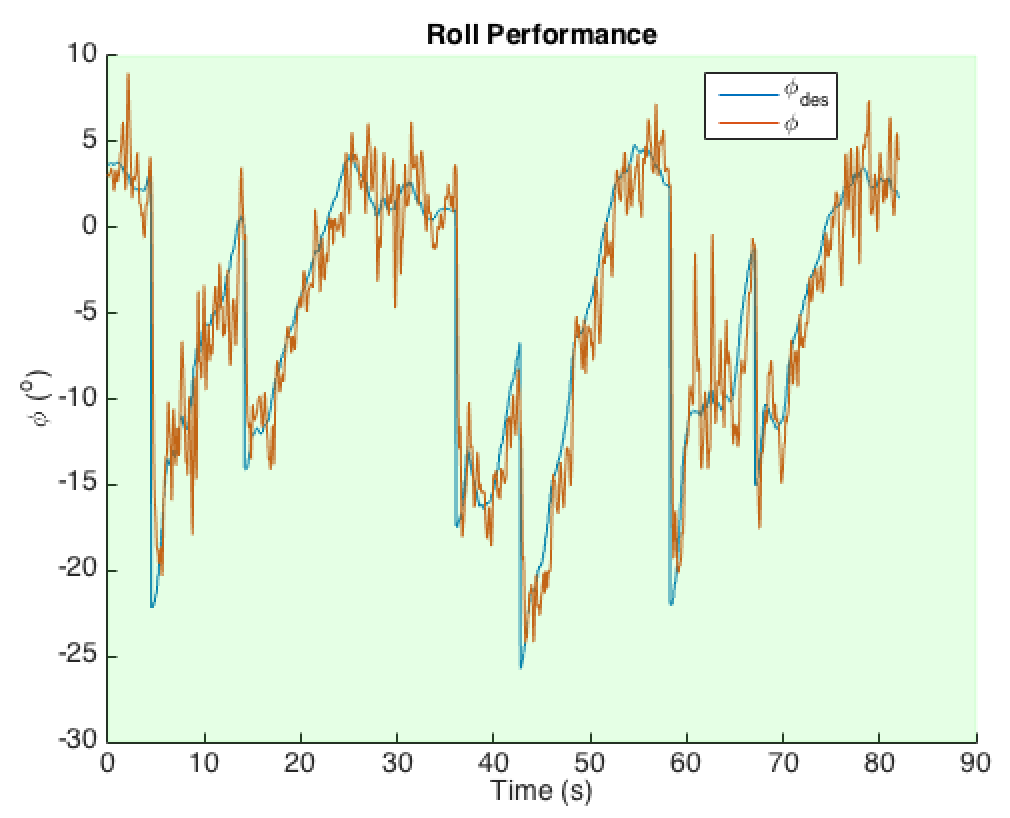
\includegraphics[width=1\textwidth]{roll_perf_flight_test.png}
  \caption{\Lone Adaptive Control Roll Performance}
  \label{fig:roll_perf_flight_test}
\end{figure}

Asymmetric flaps were configured by only allowing one servo to lower the left flap while leaving the right flap stationary.  This failure was designed to test the unmodeled roll response from a very asymmetric mechanical failure.  Unfortunately, the roll and pitch excursions caused by this failure were marginal.  Both \ac{PID} and the \Lone handled this failure with adequate reliability. 


 	%Flight Testing and Performance Evaluation
\chapter{Recommendation}\label{ch:recomendations}
This chapter provides various recommendations pertinent to the integration of the \Lone adaptive control algorithm.  These recommendations may be more qualitative than quantitative, but provide experience based guidance for the engineer to better understand the nuances of the \Lone adaptive control algorithm.  Prior to this research, there was very little experientially based guidance on implementation of this algorithm which proved to be the largest barrier for implementing this modern controller.

\section{\Lone Adaptive Control Algorithm Tuning}\label{sec:tuning}
The primary goal of this research was to reduce the complexity of tuning expertise required to get an unknown airframe airborne successfully.  The amount of time required to get the adequate airframe performance using the \Lone algorithm is significantly reduced.  Three primary features need tuning: the adaptation gain, the controller filter, and the companion model.

\subsection{Tuning the Adaptation gain}
Tuning the adaptation gain is fairly intuitive.  The adaptation gain is a function of the loop frequency at which the filter is run so it may only need to be tuned for a given autopilot at a given loop rate and not for every specific aircraft.  Anecdotally, the adaptation gain of 10,000 was used on the Pixhawk1 autopilot running the scheduled loop rate at 100Hz across multiple aircraft without needing to modify.  The primary feedback to the user for tuning this gain resides in the desired movement of the estimated states.  The adaptation gain was set low (1-10) while watching the parameters $(\theta, \omega, \sigma)$ adapt.  The adaptation gain is slowly increased until the desired rate of adaptation as seen in the real time monitoring of the parameters is adequate.  Another approach for tuning the adaptation rate is to increase the gain until parameters start to oscillate between the bounds and then reduce it.  This bang-bang response in the parameter adaptation will show up in the performance of the controller as increased peaks away from zero error between desired and achieved.  In the case of this research, this noise can be hard to identify in the rate control itself and therefore is why monitoring the attitude error helps find the appropriate adaptation gain which is extremely high but still not injecting attitude error spikes.

\subsection{Tuning the Controller Filter}
The adaptation feedback gain $(k)$, as discussed in Section~\ref{sec:l1_filter} was by far the most influential gain to tune.  The simplicity of tuning the \Lone algorithm resides in the fact that the majority of lay users could adequately tune an airframe with this stand-alone gain.  Adequate values for this gain ranged from 0.3 for responsive aircraft and 2.0 for very sluggish aircraft.  This value was set for both the roll and pitch axis independently.  As seen in Equation~\ref{eq:l1_filter}, this value is establishing the cutoff frequency of the control filter that separates the bandwidth limited control channel output and the high bandwidth adaptation.  The default value assigned in the source code was 0.45, which proved to be a good starting point.  If the default value for $k$ is not correct, then the control channel will produce either low-frequency oscillations or high-frequency oscillations.  The low-frequency oscillations are produced because the bandwidth of the control is too low and there should be a perceptible lag between the desired state and the achieved state.  High-frequency oscillations occur when the control filter bandwidth is set higher than the plant's bandwidth, and the aircraft is incapable of achieving the desired rates.  Unlike \ac{PID} control, the \Lone control never exhibited unstable performance with incorrect gains.  The controller simply oscillates with extremely poor performance.  This was a remarkable feature because poorly tuned \ac{PID} gains can cause an aircraft to depart controlled flight rapidly. Whereas, the \Lone controller maintained bounded flight performance as the theory suggests.  

\subsection{Tuning the Companion Model Cutoff Frequency}
System identification was conducted as seen in Appendix~\ref{appendix:system_identification} in order to ascertain the bandwidth of various airframes and their actuators.  Figure~\ref{fig:bode_analysis} is an example of second-order models for two aircraft's roll dynamics compared to second-order models of \ac{RC} actuators (servos).  As to be expected, the bandwidth for the actuators is slightly higher than the airframe dynamics.  
\begin{figure}[h!]
 \centering
  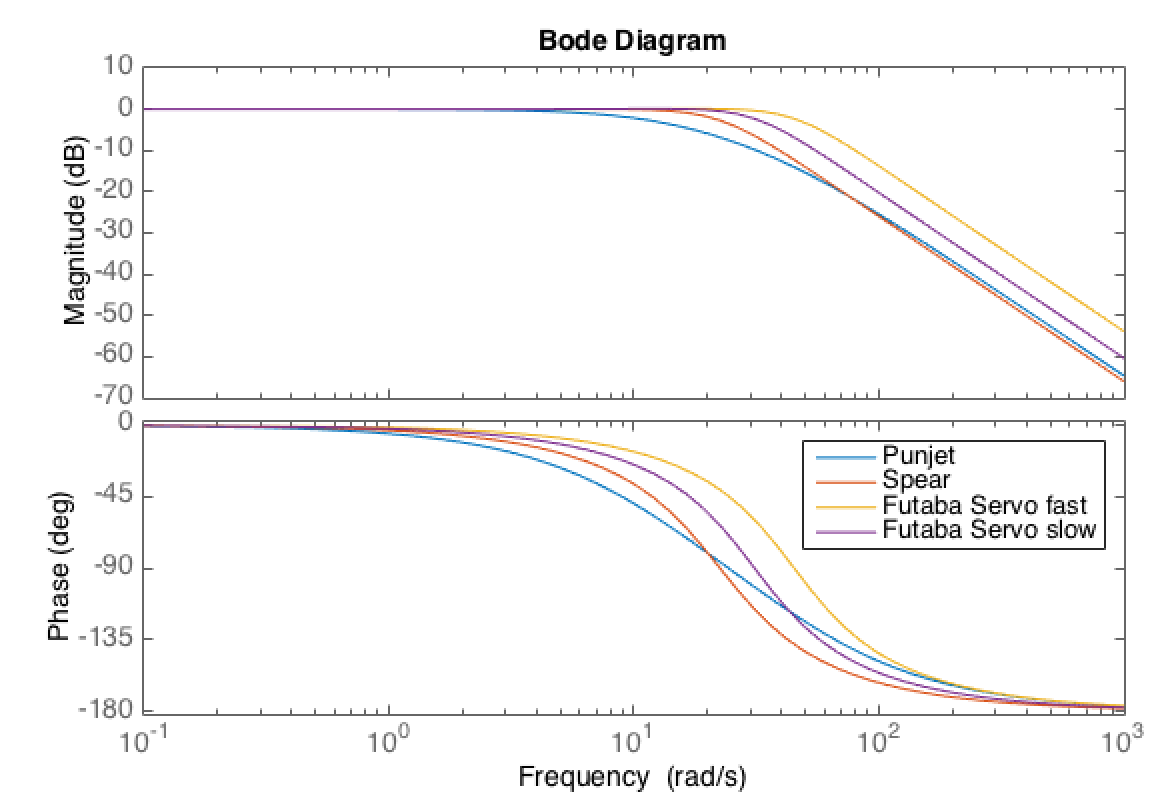
\includegraphics[width=0.85\textwidth]{bode_analysis.png}
  \caption{Aircraft Frequency Analysis }
  \label{fig:bode_analysis}
\end{figure}

These rough approximations were used to then place the cutoff frequencies of the companion model with the expectation that the companion model cannot achieve higher bandwidths than that of the airframe.  Conservatively, the companion model cutoff frequency was typically set 2-5 $rad/s$ lower than the expected max performance of the airframe.  After the other algorithm gains are tuned, and satisfactory performance is achieved, the companion model cutoff frequency can then be increased to achieve higher performance.

\section{Improved Recursive Architecture}

The speed of adaptation and accuracy of the discretized \Lone algorithm is drastically improved with increased loop frequency.  The algorithm was written as one recursive architecture that updates at the Pixhawk's scheduled loop rate.  As previously discussed, the scheduled loop rate ideally should run at lower frequencies to prevent excessive log file size and added strain on the CPU.  However, the \Lone architecture only requires the adaptation loop be run at faster rates.  With this specific performance enhancement in mind, the \ac{APM} architecture could be modified to accept an independent loop specifically for the \Lone adaptation update.  The sensors measurements and \ac{EKF} update can run significantly lower with only increased performance of the algorithm.  The higher adaptation loop would enable higher adaptation gains $(\Gamma)$ and consequently produce faster adaptation of the system.

\section{Integrator Windup Issue}
The \Lone controller architecture exhibits a similar response to integrator wind up in \ac{PID} control when the aircraft is not flying.  If the controller was enabled before takeoff, the control surfaces would move to counteract any slight deviation from input to output attempting to zero the error. Because the aircraft was not flying, the controller would continue to increase the control output until the actuators reached saturation.  The baseline code was configured to ensure that the parameter estimates would not continue to integrate after saturation was reached.  This technique is standard practice when writing control laws that utilize actuators that have saturation limitations.  However, the anti-windup feature that this offers only occurs when the actuators are saturated.  This is inadequate for the takeoff scenario.  The flight surfaces quickly saturate while waiting for takeoff and cause a crash immediately upon takeoff.  It's standard practice to also disable the integrator action of controllers if it is known that the aircraft is not flying using any combination of airspeed, throttle position, \ac{IMU} estimated velocity, or \ac{GPS} ground speed.  In the case of the \Lone algorithm, the integrator utilized in $D(s)$ is essential to the entire architecture and presented challenges in how to use ad-hoc methods to prevent the integrator windup issue even though the 'non-flying' state was calculable onboard the autopilot.  The initial experiments were to see if the adaptation rate was fast enough to un-learn the aircraft's saturated state, but there were no combinations of filter gains which resulted in learning rates adequate to ensure safe takeoffs.  Further research in this area is required to completely replace the \ac{PID} controller with the \Lone.  All takeoffs were conducted either in manual control or with the \ac{PID} controller enabled until safely airborne.

In summary, no one manual has been created for this type of controller's implementation and integration.  The recommendations provided may only apply to this specific implementation of the \Lone adaptive controller, but it offers guidance where none previously was articulated in contemporary literature.
 	%Recommendation
\chapter{Conclusion}\label{ch:conclusion}




 	%Conclusion


% APPENDICES
% You have two recommended options for your appendix:
% a) A single appendix (with a single TOC entry)
% b) Multiple appendices. Look under the examples directory for a demo of
%   multiple appendices.
%

\NPSappendices

\chapter{Projection Operator}
\label{appendix:transfer_functions}
\section{Transfer Functions}

This research utilizes the \ac{TF} representation of aircraft flight dynamics that is typical of \ac{LTI} systems.  A transfer function is a very useful approach to describe the relationship between inputs and outputs of \ac{LTI} systems.  Both analytically and numerically, the \ac{TF} approach has significant benefits in continuous and discrete time domains as its construct is based on well-developed properties and primitives of polynomials.  These polynomial representations of various aerodynamic, flight dynamics, and control properties of aircraft are well-developed.  What is unknown or partially known a priori, are the numerical values of coefficients for those polynomials. Therefore the tools from the areas of online estimation such as regression are utilized to solve for them.

Transfer functions take the form:

\begin{equation}
H(s)=\frac{Y(s)}{X(s)}\
\end{equation}

where:
\begin{itemize}
 \item[] Y(s) is the Laplace transform of the output
 \item[] X(s) is the Laplace transform of the input
\end{itemize}

Standard physics models of first and second order form are well understood and seen in many model derivations.  The first order model takes the form:

\begin{equation}\label{eq:first_order_model}
H(s)=\frac{k_{dc}}{\tau s+1}=\frac{\omega_n}{s+\omega_n}
\end{equation}

where:
\begin{itemize}
 \item[] $k_{dc}$ is the DC gain
 \item[] $\tau$ is the system time constant (time in seconds to reach 63\% of steady state)
\end{itemize}

Similarly the standard form for a second order system takes the form:

\begin{equation} \label{eq:second_order_model}
H(s)=\frac{\omega_0^2}{s^2+2\zeta\omega_0s+\omega_0^2}\
\end{equation}

where:
\begin{itemize}
 \item[] $\omega_0$ is the system natural frequency in radians per second
 \item[] $\zeta$ is the system damping ratio
\end{itemize}

The modeling of a system can also be converted to a system of first order differential equations also known as state-space modeling.  The following nomenclature will be used to illustrate the modeling of first order systems where $\dot{x}$ is the time derivative of the state, A is the Hurwitz matrix, B is the input matrix, and u is the input vector.
\begin{equation}\label{eq:state_space_model}
\dot{x}(t)=Ax(t)+Bu(t)
\end{equation}

\chapter{Matlab Code}
\label{appendix:system_identification}
\section{System Identification}

With the logged input and output data in discrete form, the data needs to be further shaped to properly convert to an s-domain representation.  The first step is ensuring that the data is of constant sampling rate.  In other words, the time between samples is uniform from sample to sample.  The data provided from the Pixhawk autopilot does not have a uniform sampling rate.  The sample rate is a user-defined rate (50-400Hz), but has a slight amount of jitter $(\pm 0.1\%)$.  \ac{PCHIP} interpolation was used to interpolate the data into a uniform sampling rate.

After the data is shaped correctly with a uniform sample rate, the discrete data is transformed into a continuous approximation using a \ac{ZOH} technique.  Taking the Laplace transform of the continuous input/output data will convert it into the s-domain and finally a non-linear least squares minimization algorithm can be run to find the polynomial coefficients which best fit the data.

The order of the regression (number of polynomials to estimate) is at the discretion of the engineer and their intuition of system's physical representation.  Higher order models will better fit the data, but in most cases tend to over fit the data if they cannot be justified by physical principles.  Most aircraft models assume that the system is \ac{LTI} and second order.  These fundamental aerodynamics models divide the modeling into longitudinal and lateral dynamics.  Essentially each axis of the aircraft is assigned two second order responses.  Pitch, for example, has a second order response in the pitch damping mode (also known as the short period) and also has a second order response in the transition of kinetic energy to potential energy (also known as the long period or phugoid).  This would imply that the collected body rate data $(\dot{p},\dot{q})$ collected by the autopilot should be modeled as first order systems because body rate is the first derivative of attitude.  Assuming a first order system for the collected data in this experiment keeps the originally derived physical meaning but may be insufficient upon critical analysis.  Both first order and second order model were estimated for comparison sake.

Results were collected from two flight test events.  The first flight test was data collected prior to implementing the chirp and the pilot attempted to increase frequency of the input signal manually.  The second set of data collected was via the reverse linear chirp method previously described.  

The manually piloted acquired data was expected to not have as adequate of frequency content in the signal but still provided adequate results for modeling the aircraft.

\begin{figure}[!h]
 \centering
  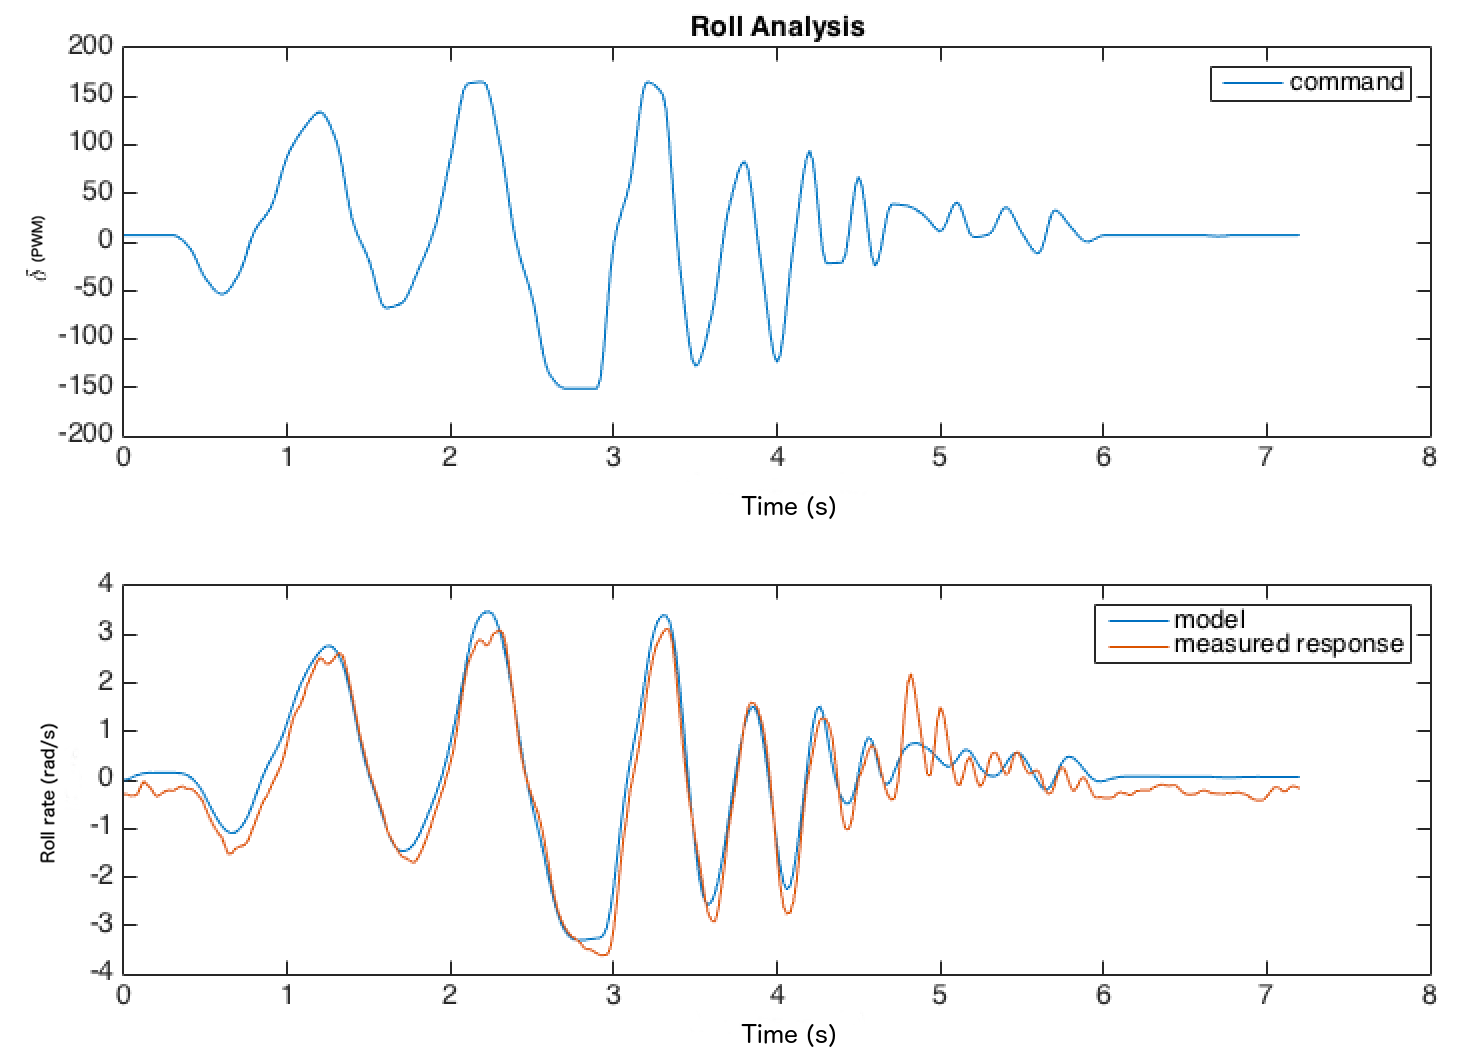
\includegraphics[width=0.75\textwidth]{model_response.png}
  \caption{Roll Model Regression with Manual Inputs}
  \label{fig:roll_model}
\end{figure}

The above result demonstrates the utility of this technique even with poorly structured data from manual pilot inputs.  It can be seen that the second order model starts to misrepresent the data at higher frequencies.  The lower frequency validity of this model showed potential and most of the high frequency response may able to be neglected upon further review.  The following figure with the chirp results highlights the actual issue with the high-frequency modeling issues.

\begin{figure}[!h]
 \centering
  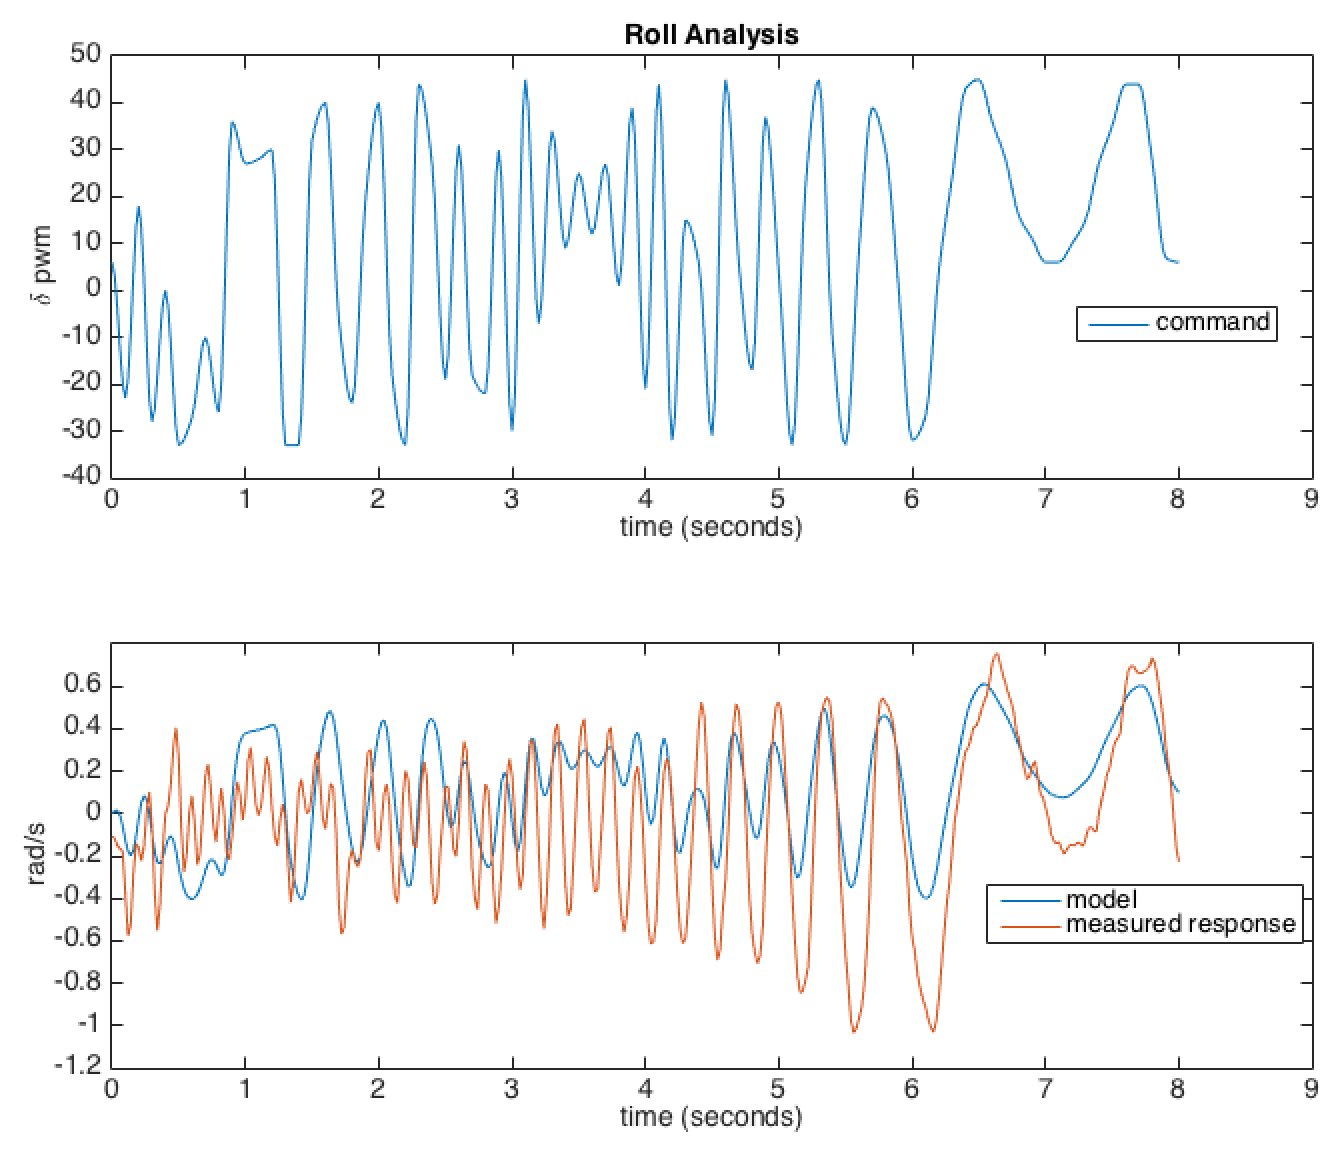
\includegraphics[width=0.75\textwidth]{chirp_response.png}
  \caption{Roll Model Regression with Reverse Linear Chirp}
  \label{fig:chirp_model}
\end{figure}

The reverse linear chirp, starting at high frequency and chirping down, clearly illustrates that this regression method has an underlying problem that was not evidently clear in the previous example.  In the chirp analysis, it is clear that the high frequency modeling is in error.  After reviewing this result, it was clear that the sampling rate of the input channel was aliased.  The chirp response was physically observed on pre-flight, in actual flight, and in the actual body rate of the aircraft.  However, the aliased input channel was arbitrarily biasing the regression result.  The data was logged at 50 Hz with the assumption that 50 Hz was 10 times higher than the expected natural frequency of the aircraft and at least five times higher than the Nyquist criterion.  The Nyquist criterion is the theoretical minimum frequency $(2f_0)$ to sample a signal and recover a given frequency.  The autopilot is capable of logging data at 400Hz, but in this case, the servo output loop is still at 50Hz due to it being the hardware bandwidth limit of standard \ac{RC} servos.  Some high performance servos are capable of higher input frequencies, but this still wouldn't solve the specific issue found when running this analysis.  The specific aliasing issue is hardware specific to the Pixhawk 1 autopilot in how the main CPU sends servo commands to the auxiliary I/O  CPU.  The most recent version of firmware at the time of this test improperly logs the \ac{PWM} through an aliased prone signal path.  The main and I/O CPU both run at 50Hz with some appreciable clock drift.  This generates a noticeable beat frequency and delay when the actual values in registry are saved for \ac{PWM} values are sent back round trip to the main CPU.  The implication of logging the pwm values at the very end of the digital transmission line seems valuable in principle because the values being logged are the undeniable values being sent to the actuators.  However, the cost of logging these values in this manner on the the Pixhawk architecture incurs significant aliasing at almost all frequencies.  Logging the commanded \ac{PWM} values prior to being sent to I/O cpu solved the aliasing discrepancy and produced very frequency rich models.

The manually piloted acquired data provided viable data source for the models even though it is a very simplistic approach.  There were two separate manual tests run on the same aircraft on the same flight and the following are the results using this regression technique to model a second order system.

\begin{equation}
H(s)=\frac{10.39}{s^2+31.26s+504.9}\
\end{equation}

and

\begin{equation}
H(s)=\frac{10.61}{s^2+29.77s+498.7}\
\end{equation}

Converting to standard form as described in equation~\ref{eq:second_order_model}:

\begin{equation}
H(s)=\frac{0.0206*22.47^2}{s^2+2*0.69*22.47s+22.47^2}\
\end{equation}

and

\begin{equation}
H(s)=\frac{0.0213*22.33^2}{s^2+2*0.67*22.33s+22.33^2}\
\end{equation}

It is important to note that this system identification technique run on separate sets of data has produced two models with very similar values for $\omega_n$ and $\zeta$.

This produces the average values of:

$\omega_n=22.4 rad/s$ \newline
$k = 0.0209$ \newline
$\zeta=0.681$ \newline

With the aliasing removed from the chirped input command signals as previously described, the model is drastically improved and produces the following results:

\begin{equation}
H(s)=\frac{4.409}{s^2+27.11s+430.6}\
\end{equation}

and

\begin{equation}
H(s)=\frac{3.295}{s^2+18.82s+2.96.5}\
\end{equation}

Converting to standard form as described in equation~\ref{eq:second_order_model}:

\begin{equation}
H(s)=\frac{0.0102*20.75^2}{s^2+2*0.65*20.75s+20.75^2}\
\end{equation}

and

\begin{equation}
H(s)=\frac{0.0111*17.21^2}{s^2+2*0.54*17.21s+17.21^2}\
\end{equation}

\begin{figure}[!h]
 \centering
  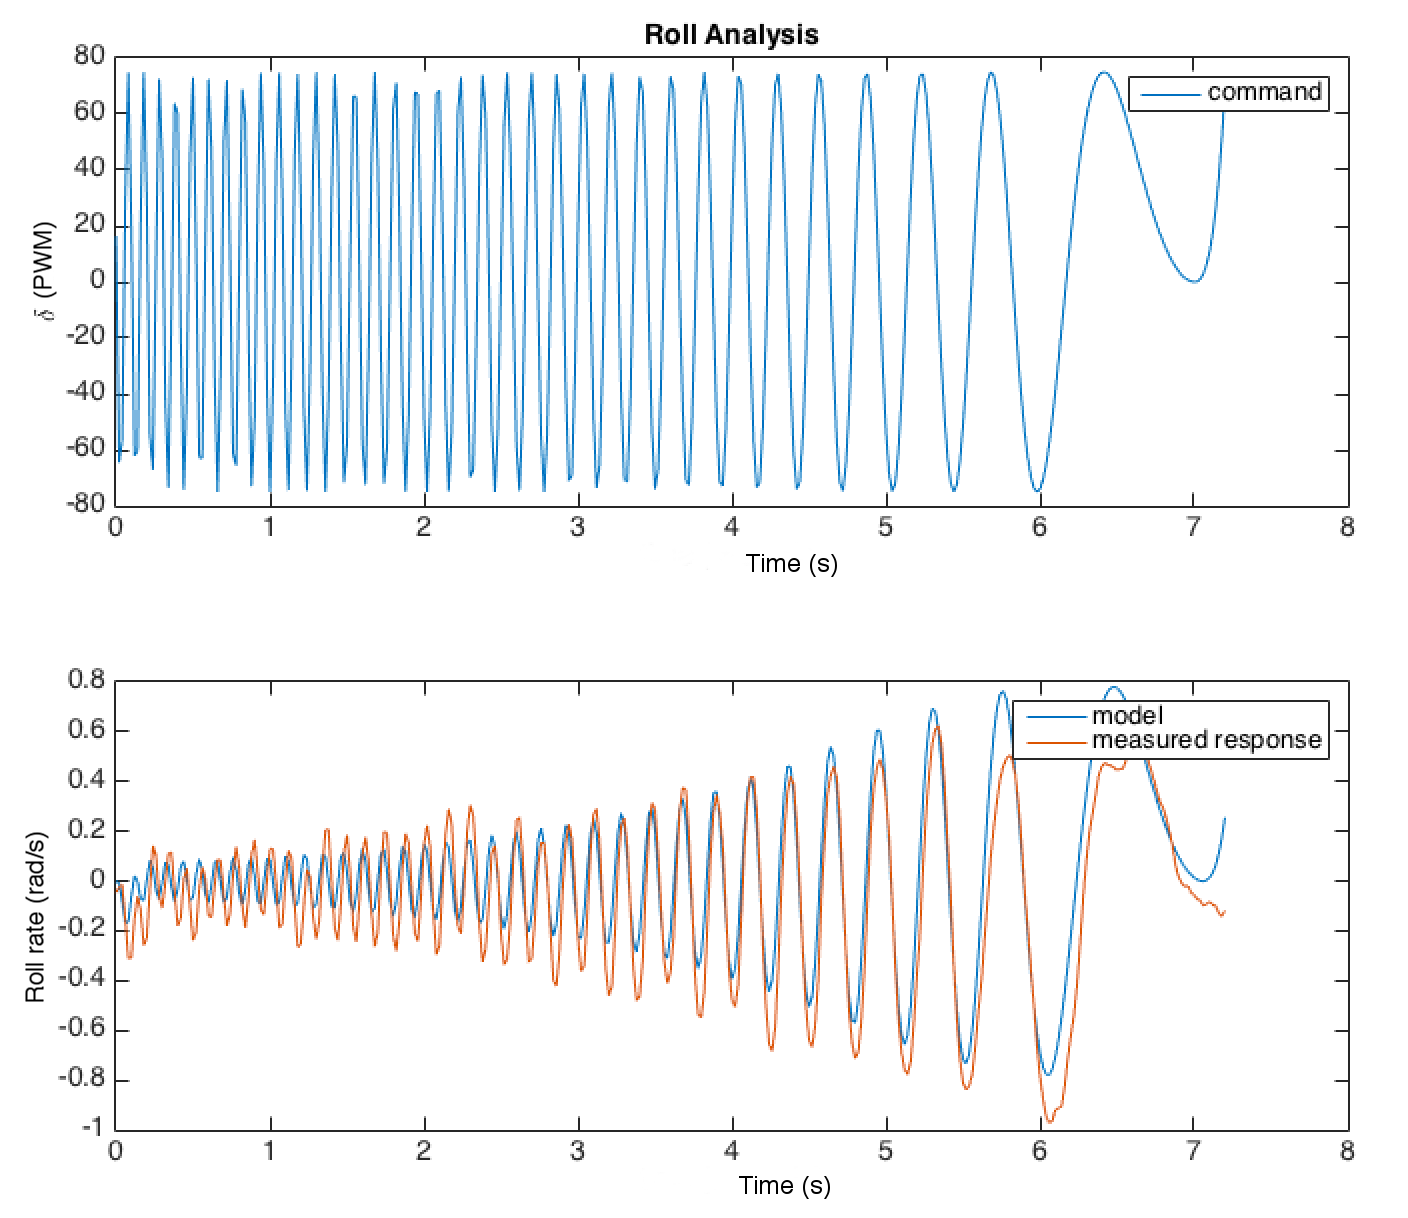
\includegraphics[width=0.75\textwidth]{reverse_chirp_roll.png}
  \caption{Non-Aliased Reverse Chirp model example}
  \label{fig:reverse_chirp_model}
\end{figure}

This produces the average values of:

$\omega_n=18.98 rad/s$ \newline
$k = 0.010$ \newline
$\zeta=0.598$ \newline

In the author's experience, these values are reasonable values for this size and weight of airframe.  This regression technique has shown potential to create realistic models from actual flight test data.  The data must be properly shaped.  The chirp method has the potential to increase the fidelity of the high frequency response of the aircraft if the aliasing issue can be resolved on the command input channel.

%\chapter{Flight Code}
%\label{appendix:system_identification}
\section{System Identification}

With the logged input and output data in discrete form, the data needs to be further shaped to properly convert to an s-domain representation.  The first step is ensuring that the data is of constant sampling rate.  In other words, the time between samples is uniform from sample to sample.  The data provided from the Pixhawk autopilot does not have a uniform sampling rate.  The sample rate is a user-defined rate (50-400Hz), but has a slight amount of jitter $(\pm 0.1\%)$.  \ac{PCHIP} interpolation was used to interpolate the data into a uniform sampling rate.

After the data is shaped correctly with a uniform sample rate, the discrete data is transformed into a continuous approximation using a \ac{ZOH} technique.  Taking the Laplace transform of the continuous input/output data will convert it into the s-domain and finally a non-linear least squares minimization algorithm can be run to find the polynomial coefficients which best fit the data.

The order of the regression (number of polynomials to estimate) is at the discretion of the engineer and their intuition of system's physical representation.  Higher order models will better fit the data, but in most cases tend to over fit the data if they cannot be justified by physical principles.  Most aircraft models assume that the system is \ac{LTI} and second order.  These fundamental aerodynamics models divide the modeling into longitudinal and lateral dynamics.  Essentially each axis of the aircraft is assigned two second order responses.  Pitch, for example, has a second order response in the pitch damping mode (also known as the short period) and also has a second order response in the transition of kinetic energy to potential energy (also known as the long period or phugoid).  This would imply that the collected body rate data $(\dot{p},\dot{q})$ collected by the autopilot should be modeled as first order systems because body rate is the first derivative of attitude.  Assuming a first order system for the collected data in this experiment keeps the originally derived physical meaning but may be insufficient upon critical analysis.  Both first order and second order model were estimated for comparison sake.

Results were collected from two flight test events.  The first flight test was data collected prior to implementing the chirp and the pilot attempted to increase frequency of the input signal manually.  The second set of data collected was via the reverse linear chirp method previously described.  

The manually piloted acquired data was expected to not have as adequate of frequency content in the signal but still provided adequate results for modeling the aircraft.

\begin{figure}[!h]
 \centering
  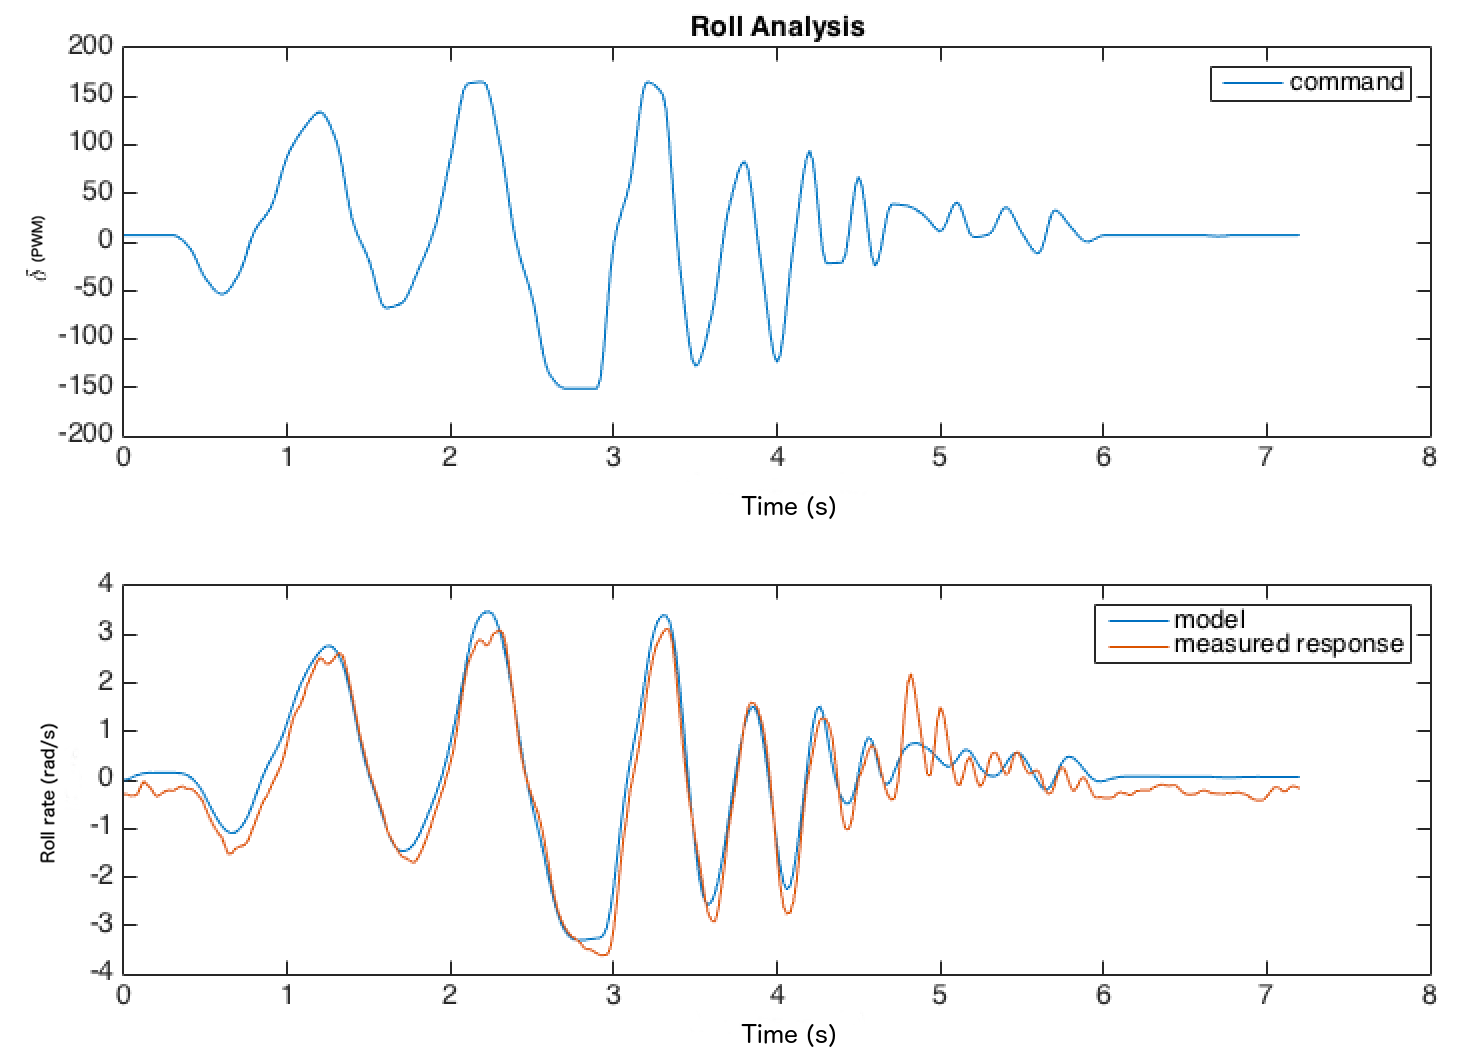
\includegraphics[width=0.75\textwidth]{model_response.png}
  \caption{Roll Model Regression with Manual Inputs}
  \label{fig:roll_model}
\end{figure}

The above result demonstrates the utility of this technique even with poorly structured data from manual pilot inputs.  It can be seen that the second order model starts to misrepresent the data at higher frequencies.  The lower frequency validity of this model showed potential and most of the high frequency response may able to be neglected upon further review.  The following figure with the chirp results highlights the actual issue with the high-frequency modeling issues.

\begin{figure}[!h]
 \centering
  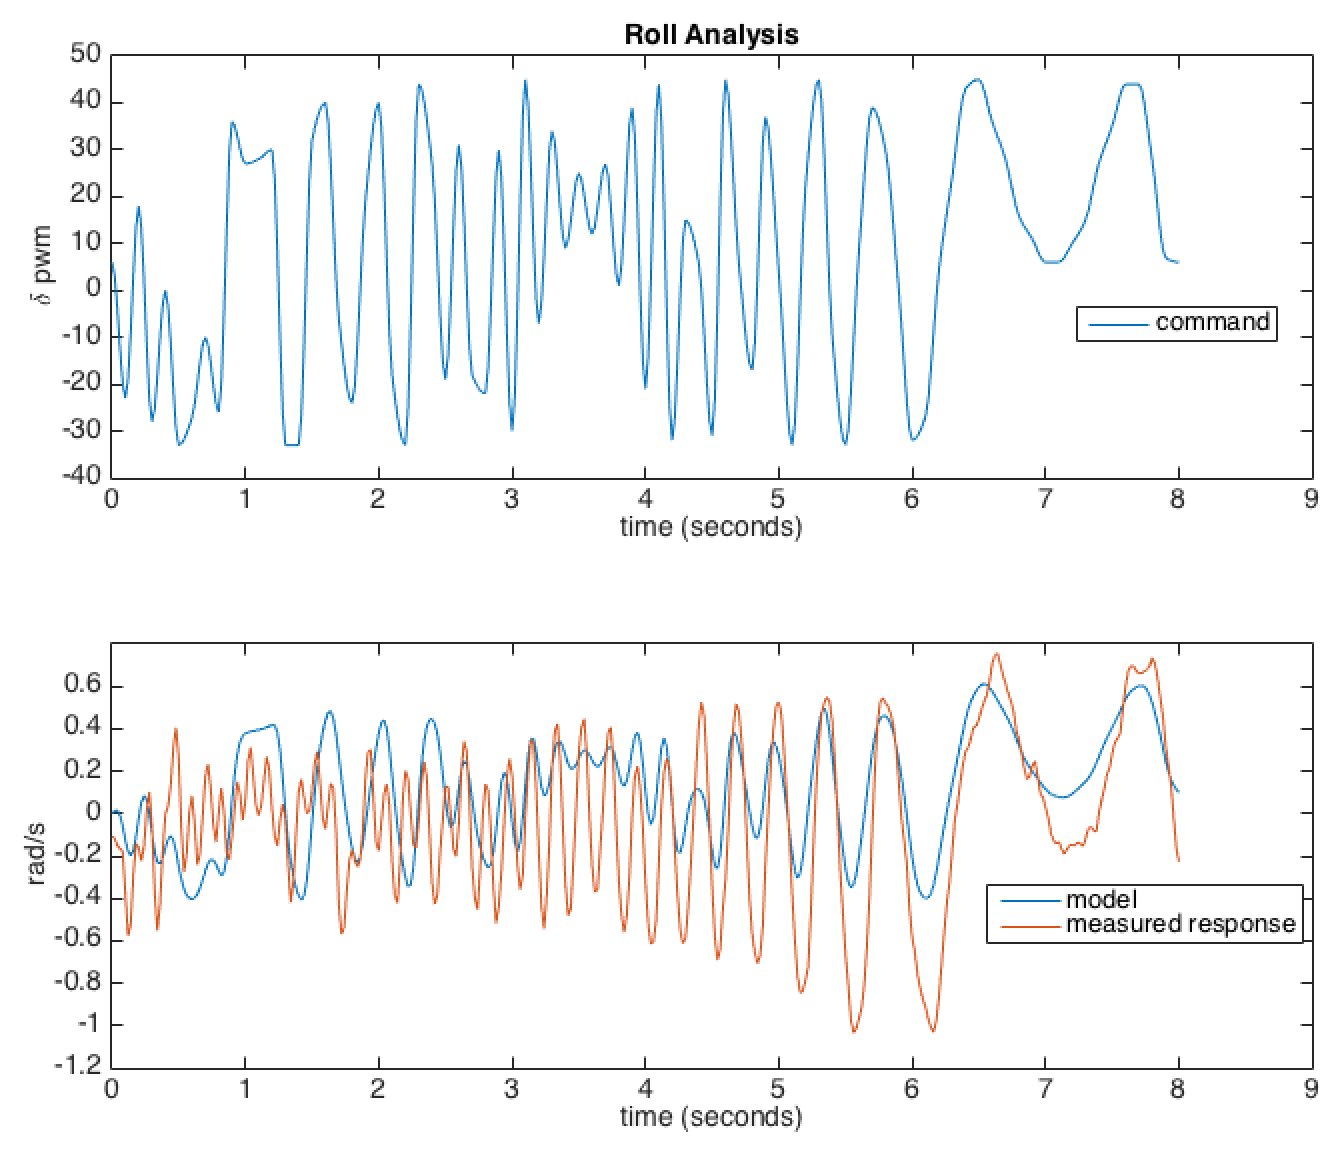
\includegraphics[width=0.75\textwidth]{chirp_response.png}
  \caption{Roll Model Regression with Reverse Linear Chirp}
  \label{fig:chirp_model}
\end{figure}

The reverse linear chirp, starting at high frequency and chirping down, clearly illustrates that this regression method has an underlying problem that was not evidently clear in the previous example.  In the chirp analysis, it is clear that the high frequency modeling is in error.  After reviewing this result, it was clear that the sampling rate of the input channel was aliased.  The chirp response was physically observed on pre-flight, in actual flight, and in the actual body rate of the aircraft.  However, the aliased input channel was arbitrarily biasing the regression result.  The data was logged at 50 Hz with the assumption that 50 Hz was 10 times higher than the expected natural frequency of the aircraft and at least five times higher than the Nyquist criterion.  The Nyquist criterion is the theoretical minimum frequency $(2f_0)$ to sample a signal and recover a given frequency.  The autopilot is capable of logging data at 400Hz, but in this case, the servo output loop is still at 50Hz due to it being the hardware bandwidth limit of standard \ac{RC} servos.  Some high performance servos are capable of higher input frequencies, but this still wouldn't solve the specific issue found when running this analysis.  The specific aliasing issue is hardware specific to the Pixhawk 1 autopilot in how the main CPU sends servo commands to the auxiliary I/O  CPU.  The most recent version of firmware at the time of this test improperly logs the \ac{PWM} through an aliased prone signal path.  The main and I/O CPU both run at 50Hz with some appreciable clock drift.  This generates a noticeable beat frequency and delay when the actual values in registry are saved for \ac{PWM} values are sent back round trip to the main CPU.  The implication of logging the pwm values at the very end of the digital transmission line seems valuable in principle because the values being logged are the undeniable values being sent to the actuators.  However, the cost of logging these values in this manner on the the Pixhawk architecture incurs significant aliasing at almost all frequencies.  Logging the commanded \ac{PWM} values prior to being sent to I/O cpu solved the aliasing discrepancy and produced very frequency rich models.

The manually piloted acquired data provided viable data source for the models even though it is a very simplistic approach.  There were two separate manual tests run on the same aircraft on the same flight and the following are the results using this regression technique to model a second order system.

\begin{equation}
H(s)=\frac{10.39}{s^2+31.26s+504.9}\
\end{equation}

and

\begin{equation}
H(s)=\frac{10.61}{s^2+29.77s+498.7}\
\end{equation}

Converting to standard form as described in equation~\ref{eq:second_order_model}:

\begin{equation}
H(s)=\frac{0.0206*22.47^2}{s^2+2*0.69*22.47s+22.47^2}\
\end{equation}

and

\begin{equation}
H(s)=\frac{0.0213*22.33^2}{s^2+2*0.67*22.33s+22.33^2}\
\end{equation}

It is important to note that this system identification technique run on separate sets of data has produced two models with very similar values for $\omega_n$ and $\zeta$.

This produces the average values of:

$\omega_n=22.4 rad/s$ \newline
$k = 0.0209$ \newline
$\zeta=0.681$ \newline

With the aliasing removed from the chirped input command signals as previously described, the model is drastically improved and produces the following results:

\begin{equation}
H(s)=\frac{4.409}{s^2+27.11s+430.6}\
\end{equation}

and

\begin{equation}
H(s)=\frac{3.295}{s^2+18.82s+2.96.5}\
\end{equation}

Converting to standard form as described in equation~\ref{eq:second_order_model}:

\begin{equation}
H(s)=\frac{0.0102*20.75^2}{s^2+2*0.65*20.75s+20.75^2}\
\end{equation}

and

\begin{equation}
H(s)=\frac{0.0111*17.21^2}{s^2+2*0.54*17.21s+17.21^2}\
\end{equation}

\begin{figure}[!h]
 \centering
  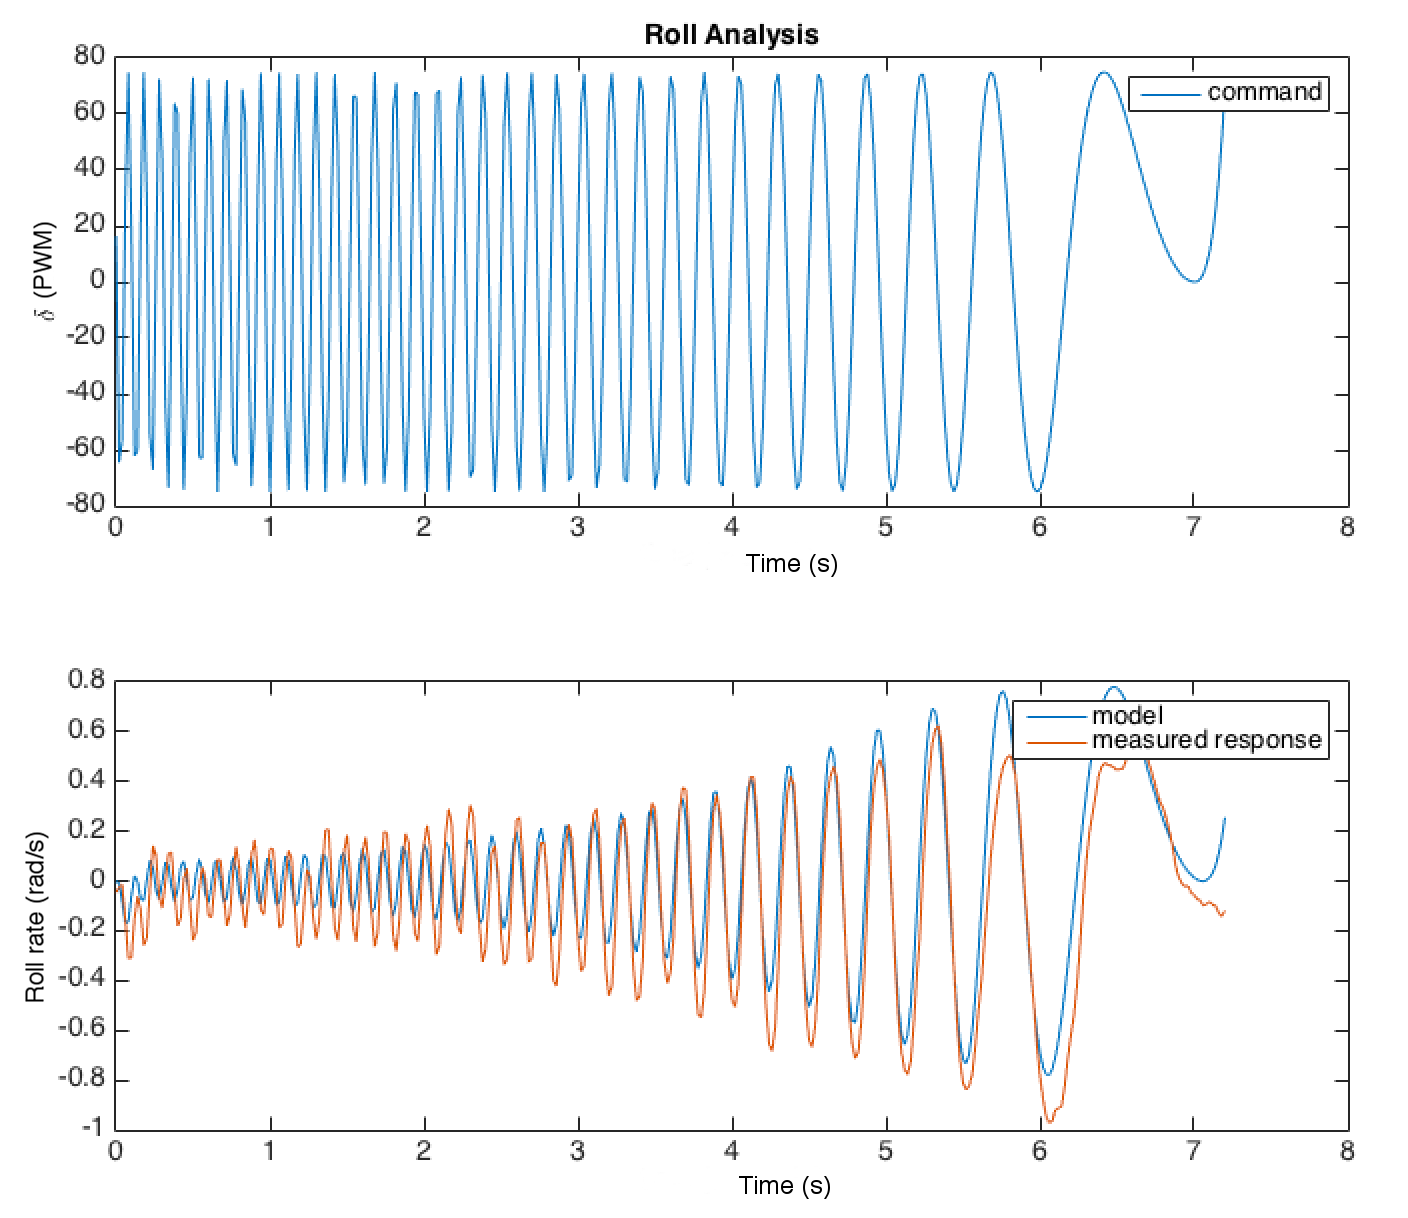
\includegraphics[width=0.75\textwidth]{reverse_chirp_roll.png}
  \caption{Non-Aliased Reverse Chirp model example}
  \label{fig:reverse_chirp_model}
\end{figure}

This produces the average values of:

$\omega_n=18.98 rad/s$ \newline
$k = 0.010$ \newline
$\zeta=0.598$ \newline

In the author's experience, these values are reasonable values for this size and weight of airframe.  This regression technique has shown potential to create realistic models from actual flight test data.  The data must be properly shaped.  The chirp method has the potential to increase the fidelity of the high frequency response of the aircraft if the aliasing issue can be resolved on the command input channel.

% REFERENCES
% List all your BibTeX reference source files (ending in *.bib extension)
%
\NPSbibliography{thesis}


%
% This is the official end of the thesis.
%
\NPSend

% DISTRIBUTION LIST
% The list is automatically properly numbered
% and already populated with the mandatory recipients.
%
\NPSdistribution{Initial Distribution List}
\begin{distributionlist}
\item Defense Technical Information Center\\Ft. Belvoir, Virginia
\item Dudley Knox Library\\Naval Postgraduate School\\Monterey, California
%
%---- Other entries are no longer needed, because of Special Abstract Form
% Marine Corps students are required to show:
%\item Marine Corps Representative\\Naval Postgraduate School\\Monterey, California
%\item Directory, Training and Education, MCCDC, Code C46\\Quantico, Virginia
%\item Marine Corps Tactical System Support Activity (Attn: Operations Officer)\\Camp Pendleton, California
%
% Officer students in the Operations Research Program are also required to show:
%\item Director, Studies and Analysis Division, MCCDC, Code C45\\ Quantico, Virginia
%
% Officer students in the Space Ops/Space Engineering Program or in the Information Warfare/Information Systems and Operations are also required to show:
%\item Head, Information Operations and Space Integration Branch,\\ PLI/PP\&O/HQMC, Washington, DC
\end{distributionlist}


\end{document}

